%!LW recipe=latexmk (xelatex)
%!TEX program = xelatex
%!TEX root = report.tex
% Compile from docs/ (or from the repository root via docs/report.tex).
% Assets: images/hcmut.png and diagrams/*.png; see README.md for offline setup.
% Consolidated specification: seven chapters; no external TeX input is required.
\documentclass[12pt,a4paper]{report}
\usepackage[a4paper,top=2.5cm,bottom=2.4cm,left=2.5cm,right=2.2cm,headheight=32pt,headsep=12pt]{geometry}
\usepackage{iftex}
\ifPDFTeX
  \usepackage[utf8]{inputenc}
  \usepackage[T5]{fontenc}
  \usepackage{lmodern}
\else
  \usepackage{fontspec}
  \IfFontExistsTF{Times New Roman}{\setmainfont{Times New Roman}}{\setmainfont{Latin Modern Roman}}
  \IfFontExistsTF{Arial}{\setsansfont{Arial}}{\setsansfont{Latin Modern Sans}}
\fi

\usepackage{amsmath,amssymb}
\usepackage{graphicx}
\usepackage{float}
\usepackage{pdflscape,caption}
\graphicspath{{./}{docs/}}
\usepackage{xcolor}
\usepackage{array}
\usepackage{longtable}
\usepackage{tabularx}
\usepackage{booktabs}
\usepackage{enumitem}
\usepackage{tikz}
\usetikzlibrary{calc}
\usepackage{fancyhdr}
\usepackage{lastpage}
\usepackage{url}
\urlstyle{same}
\usepackage{hyperref}

\definecolor{bkblue}{HTML}{0B3B91}
\definecolor{bkuBlue}{RGB}{11,43,115}
\definecolor{needcolor}{HTML}{A33A00}
\hypersetup{colorlinks=true,linkcolor=bkblue,urlcolor=bkblue}

\setlength{\parindent}{0pt}
\setlength{\parskip}{0.55\baselineskip}
\setlength{\emergencystretch}{3em}
\setlist{nosep,leftmargin=1.6em}
\renewcommand{\chaptername}{CHƯƠNG}
\renewcommand{\contentsname}{MỤC LỤC}
\renewcommand{\tablename}{Bảng}
\renewcommand{\figurename}{Hình}
\renewcommand{\listfigurename}{DANH MỤC SƠ ĐỒ VÀ HÌNH}
\renewcommand{\partname}{PHẦN}
\captionsetup{font=small,labelfont=bf,hypcap=false}
\renewcommand{\arraystretch}{1.25}
\setcounter{tocdepth}{2}
\setcounter{secnumdepth}{3}

\newcommand{\req}[1]{\textbf{#1}}
\newcommand{\yes}{X}
\newcommand{\code}[1]{\texttt{\detokenize{#1}}}
\newcommand{\diagramtext}[1]{\begingroup\clubpenalty=10000\widowpenalty=10000 #1\par\endgroup}

% ==========================================
%         HEADER & FOOTER (fancyhdr)
% ==========================================
\pagestyle{fancy}
\fancyhf{}
\setlength{\headheight}{32pt}
\setlength{\footskip}{20pt}

\fancyhead[L]{%
  \begin{minipage}[c]{9mm}
    
\includegraphics[width=8mm,height=8mm,keepaspectratio]{images/hcmut.png}
  \end{minipage}%
  \hspace{2mm}%
  \begin{minipage}[c]{0.78\textwidth}
    \fontsize{8.5pt}{11pt}\selectfont\ttfamily
    Trường Đại học Bách Khoa --- ĐHQG TP.HCM \\
    Khoa Khoa học và Kỹ thuật Máy tính
  \end{minipage}%
}
\fancyhead[R]{}

\fancyfoot[L]{%
  \fontsize{9pt}{11pt}\selectfont
  Đồ án Chuyên ngành (CO4029) --- TASS
}
\fancyfoot[R]{%
  \fontsize{9pt}{11pt}\selectfont
  Trang \thepage/\pageref*{LastPage}
}

\renewcommand{\headrulewidth}{0.4pt}
\renewcommand{\footrulewidth}{0.4pt}

% Đồng bộ cho cả trang mở đầu chapter (mặc định LaTeX dùng plain)
\fancypagestyle{plain}{%
  \fancyhf{}
  \fancyhead[L]{%
    \begin{minipage}[c]{9mm}
      
\includegraphics[width=8mm,height=8mm,keepaspectratio]{images/hcmut.png}
    \end{minipage}%
    \hspace{2mm}%
    \begin{minipage}[c]{0.78\textwidth}
      \fontsize{8.5pt}{11pt}\selectfont\ttfamily
      Trường Đại học Bách Khoa --- ĐHQG TP.HCM \\
      Khoa Khoa học và Kỹ thuật Máy tính
    \end{minipage}%
  }
  \fancyfoot[L]{\fontsize{9pt}{11pt}\selectfont Đồ án Chuyên ngành (CO4029) --- TASS}
  \fancyfoot[R]{\fontsize{9pt}{11pt}\selectfont Trang \thepage/\pageref*{LastPage}}
  \renewcommand{\headrulewidth}{0.4pt}
  \renewcommand{\footrulewidth}{0.4pt}
}

\begin{document}

% ==========================================
%    TRANG BÌA CÓ KHUNG MÀU XANH BÁCH KHOA
% ==========================================
\begin{titlepage}
\thispagestyle{empty}
\begin{tikzpicture}[remember picture, overlay]
  % Tọa độ 4 góc ngoài (cách mép giấy 1.3cm)
  \coordinate (TL) at ($(current page.north west) + (1.3cm,-1.3cm)$);
  \coordinate (TR) at ($(current page.north east) + (-1.3cm,-1.3cm)$);
  \coordinate (BL) at ($(current page.south west) + (1.3cm,1.3cm)$);
  \coordinate (BR) at ($(current page.south east) + (-1.3cm,1.3cm)$);
  
  % Tọa độ 4 góc trong (cách góc ngoài 1.8mm)
  \coordinate (TL_in) at ($(current page.north west) + (1.48cm,-1.48cm)$);
  \coordinate (TR_in) at ($(current page.north east) + (-1.48cm,-1.48cm)$);
  \coordinate (BL_in) at ($(current page.south west) + (1.48cm,1.48cm)$);
  \coordinate (BR_in) at ($(current page.south east) + (-1.48cm,1.48cm)$);

  % Viền ngoài và viền trong màu xanh Bách Khoa
  \draw[line width=2.8pt, color=bkuBlue] (TL) rectangle (BR);
  \draw[line width=1.0pt, color=bkuBlue] (TL_in) rectangle (BR_in);

  % Họa tiết 4 góc vuông kiểu trang bìa chuẩn Bách Khoa
  \draw[line width=1pt, color=bkuBlue, fill=bkuBlue] (TL) rectangle ++(0.35cm, -0.35cm);
  \draw[line width=0.8pt, color=white, fill=white] ($(TL)+(0.06cm,-0.06cm)$) rectangle ++(0.23cm, -0.23cm);
  \draw[line width=0.6pt, color=bkuBlue, fill=bkuBlue] ($(TL)+(0.12cm,-0.12cm)$) rectangle ++(0.11cm, -0.11cm);

  \draw[line width=1pt, color=bkuBlue, fill=bkuBlue] (TR) rectangle ++(-0.35cm, -0.35cm);
  \draw[line width=0.8pt, color=white, fill=white] ($(TR)+(-0.06cm,-0.06cm)$) rectangle ++(-0.23cm, -0.23cm);
  \draw[line width=0.6pt, color=bkuBlue, fill=bkuBlue] ($(TR)+(-0.12cm,-0.12cm)$) rectangle ++(-0.11cm, -0.11cm);

  \draw[line width=1pt, color=bkuBlue, fill=bkuBlue] (BL) rectangle ++(0.35cm, 0.35cm);
  \draw[line width=0.8pt, color=white, fill=white] ($(BL)+(0.06cm,0.06cm)$) rectangle ++(0.23cm, 0.23cm);
  \draw[line width=0.6pt, color=bkuBlue, fill=bkuBlue] ($(BL)+(0.12cm,0.12cm)$) rectangle ++(0.11cm, 0.11cm);

  \draw[line width=1pt, color=bkuBlue, fill=bkuBlue] (BR) rectangle ++(-0.35cm, 0.35cm);
  \draw[line width=0.8pt, color=white, fill=white] ($(BR)+(-0.06cm,0.06cm)$) rectangle ++(-0.23cm, 0.23cm);
  \draw[line width=0.6pt, color=bkuBlue, fill=bkuBlue] ($(BR)+(-0.12cm,0.12cm)$) rectangle ++(-0.11cm, 0.11cm);
\end{tikzpicture}

\begin{center}
  {\fontsize{13pt}{16pt}\selectfont\textbf{ĐẠI HỌC QUỐC GIA THÀNH PHỐ HỒ CHÍ MINH}\par}
  \vspace{0.12cm}
  {\fontsize{13pt}{16pt}\selectfont\textbf{TRƯỜNG ĐẠI HỌC BÁCH KHOA}\par}
  \vspace{0.12cm}
  {\fontsize{13pt}{16pt}\selectfont\textbf{KHOA KHOA HỌC VÀ KỸ THUẬT MÁY TÍNH}\par}

  \vspace{0.6cm}
  
\includegraphics[width=3.6cm]{images/hcmut.png}\par
  \vspace{0.6cm}

  {\fontsize{14pt}{18pt}\selectfont\textbf{BÁO CÁO ĐỒ ÁN CHUYÊN NGÀNH (CO4029)}\par}
  \vspace{0.35cm}
  {\fontsize{20pt}{24pt}\selectfont\bfseries\color{bkuBlue} YÊU CẦU HỆ THỐNG\\ VÀ THIẾT KẾ THUẬT TOÁN\par}
  \vspace{0.25cm}
  {\fontsize{15pt}{19pt}\selectfont\bfseries HỆ THỐNG HỖ TRỢ PHÂN CÔNG GIẢNG DẠY (TASS)\par}
  \vspace{0.15cm}
  {\fontsize{12pt}{15pt}\selectfont\itshape Teaching Assignment Support System\par}
  \vspace{0.3cm}
  {\fontsize{11pt}{14pt}\selectfont\textbf{Đặc tả yêu cầu và thiết kế thuật toán --- 31/10/2026}\par}

  \vfill

  \begin{tabular}{rp{7.8cm}}
    \textbf{Giáo viên hướng dẫn:} & ThS. Mai Đức Trung (003710) \\
  \end{tabular}

  \vspace{0.35cm}

  \begin{tabular}{|c|p{5.5cm}|p{6.0cm}|}
    \hline
    \textbf{MSSV} & \textbf{Họ và tên} & \textbf{Email} \\
    \hline
    2152435 & Hà Thế Bình & binh.hathe@hcmut.edu.vn \\
    \hline
    2311628 & Nguyễn Trần Đức Duy Khoa & khoa.nguyentran@hcmut.edu.vn \\
    \hline
    2311514 & Nguyễn Gia Khánh & khanh.nguyengia@hcmut.edu.vn \\
    \hline
  \end{tabular}

  \vfill
  {\fontsize{11pt}{14pt}\selectfont\textbf{TP. HỒ CHÍ MINH, THÁNG 10/2026}\par}
\end{center}
\end{titlepage}

\hypersetup{pageanchor=true}
\pagenumbering{roman}
\begingroup\small\tableofcontents\endgroup
\clearpage
\begingroup\small
\listoffigures
\addcontentsline{toc}{chapter}{\listfigurename}
\endgroup
\clearpage

\pagenumbering{arabic}
\setcounter{page}{1}

\chapter{GIỚI THIỆU VÀ TỔNG QUAN}\label{chap:introduction}

\section{Mục đích}
TASS (Teaching Assignment Support System) hỗ trợ phân công giáo viên theo học kỳ: chuẩn bị dữ liệu, sinh đề xuất, chỉnh sửa, kiểm tra tải, lấy phản hồi và xuất phương án đề xuất. Báo cáo là cơ sở thiết kế, triển khai và kiểm chứng; mức độ hiện thực và kết quả kiểm chứng được trình bày tại Chương~\ref{chap:verification}.

\section{Phạm vi MVP}\label{sec:mvp}
Mỗi đợt thuộc một đơn vị và học kỳ, có một phương án hiện hành và lịch sử phiên bản chỉ đọc. Đơn vị phân công là thành phần nhu cầu theo lớp--môn--học kỳ--giai đoạn. Mỗi thành phần có tối đa một giáo viên; phương án hoàn chỉnh phải đáp ứng toàn bộ thành phần bắt buộc.

Phiên bản tối thiểu khả dụng (MVP) cung cấp các chức năng quản lý tài khoản và dữ liệu nền; xác nhận phạm vi môn học, khối lớp, chuyên môn, nhu cầu và tải giảng dạy; sinh đề xuất tự động, chỉnh sửa thủ công và khóa phân công. Hệ thống còn hỗ trợ kiểm tra ràng buộc, cân bằng tải, tiếp nhận phản hồi cá nhân và xuất PDF theo giáo viên hoặc lớp học. Chức năng sinh đề xuất tự động là yêu cầu bắt buộc. Các nhu cầu STANDARD, SPECIALIZED\_TOPIC và ENRICHMENT thuộc từng lớp riêng. KHTN (Khoa học tự nhiên) là một môn học độc lập trong danh mục, được quản lý như Toán hoặc Vật lý và áp dụng quy tắc một giáo viên cho mỗi thành phần nhu cầu theo hiệu lực. Việc tính định mức trong MVP áp dụng cho giáo viên THCS và THPT theo chế độ thông thường.

\section{Ngoài phạm vi MVP}\label{sec:out-of-scope}
MVP chưa bao gồm chức năng xếp thời khóa biểu theo ngày, buổi, tiết học và phòng học; quản lý nguyện vọng hoặc lịch bận cá nhân; tổ chức nhóm lớp ghép và tính tải chung cho nhiều lớp; phân công KHTN theo từng mạch nội dung; phân công nhiều giáo viên cùng phụ trách một thành phần nhu cầu; tạo nhiều phương án song song; phê duyệt chính thức; hoặc tính lương dạy thêm giờ. Các chế độ TLTN, thỉnh giảng và hợp đồng, cùng việc thẩm định đầy đủ các chế độ đặc thù, thuộc phạm vi mở rộng. Trong phiên bản hiện tại, Excel chỉ phục vụ đối chiếu và chuẩn bị dữ liệu kiểm chứng; hệ thống chưa hỗ trợ nhập Excel hàng loạt hoặc tích hợp FET và vnEdu.

\section{Tài liệu tham chiếu}\label{sec:reference-documents}
Các quy tắc về chế độ làm việc và định mức giảng dạy được tham chiếu từ [4]; chế độ công tác công đoàn từ [7]; chương trình môn học từ [9]; và điều lệ trường từ [21]. Những văn bản liên quan được dẫn tại từng quy tắc cụ thể. Mô hình thuật toán sử dụng các tài liệu [22]--[28], còn dữ liệu đối chiếu gồm ba workbook [29]--[31], trong đó E3 năm học 2026--2027 là nguồn chuẩn. Danh sách tài liệu và liên kết được trình bày tại phần \hyperref[chap:references]{Tài liệu tham khảo}.

\section{Vai trò và bối cảnh sử dụng}\label{sec:overview}

\begin{longtable}{|p{3.3cm}|p{10.6cm}|}
\hline
\textbf{Vai trò} & \textbf{Trách nhiệm} \\\hline
\endfirsthead
\hline
\textbf{Vai trò} & \textbf{Trách nhiệm} \\\hline
\endhead
Administrator & Quản lý tài khoản, vai trò, danh mục, năm học/học kỳ và dữ liệu nền theo quyền; không mặc định là người lập phương án. \\\hline
Academic Manager & Chuẩn bị đợt, sinh/chỉnh/kiểm tra phương án, mở/xử lý phản hồi và xuất đề xuất; có thể là Ban Giám hiệu, tổ trưởng hoặc giáo vụ được ủy quyền. \\\hline
Teacher & Xem phân công và tải cá nhân khi được mở, phản hồi trong hạn và theo dõi kết quả của mình; không sửa phương án hoặc xem dữ liệu người khác. \\\hline
\end{longtable}



Từ phạm vi và trách nhiệm của các vai trò, Hình~\ref{fig:DG-01} xác định ranh giới TASS và các luồng thông tin qua ranh giới đó. Hệ thống nhận dữ liệu quản trị, yêu cầu phân công và phản hồi để trả lại kết quả phù hợp với từng nhóm người dùng.

\begin{figure}[H]
\centering
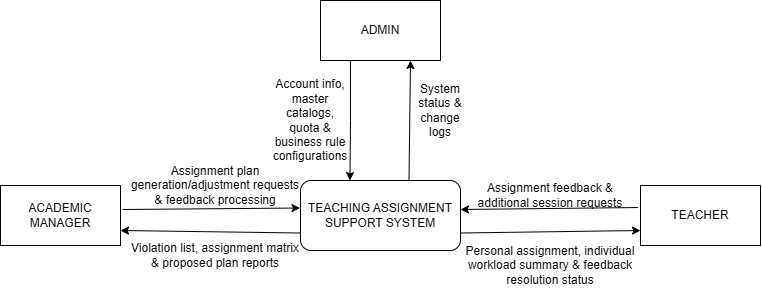
\includegraphics[width=0.98\linewidth,height=0.36\textheight,keepaspectratio]{diagrams/DG-01.png}
\caption{DG-01 --- Sơ đồ ngữ cảnh}\label{fig:DG-01}
\end{figure}

\diagramtext{Administrator cung cấp danh mục, định mức và quy tắc; Academic Manager yêu cầu lập/chỉnh phương án và nhận ma trận phân công, vi phạm cùng báo cáo đề xuất. Teacher chỉ nhận phân công và tải cá nhân và gửi phản hồi; luồng đề nghị nhận thêm tiết được hiểu theo FR-20, không tự tạo nhu cầu mới.}


\section{Môi trường và cấu trúc báo cáo}\label{sec:environment}
Ứng dụng web dùng máy chủ và cơ sở dữ liệu bền vững. Số tiết nhu cầu là đầu vào, không suy từ thời khóa biểu; phải kiểm tra dữ liệu, hiệu lực và năng lực trước khi giải. Kiến trúc đề xuất tại Mục~\ref{sec:deployment}.

Báo cáo gồm bảy chương. Sau phần giới thiệu, Chương~\ref{chap:business} phân tích mô hình nghiệp vụ; Chương~\ref{chap:functional} đặc tả yêu cầu hệ thống; Chương~\ref{chap:data} trình bày thiết kế dữ liệu và kiến trúc; Chương~\ref{chap:math-model} mô hình hóa bài toán phân công; Chương~\ref{chap:verification} đánh giá khả năng kiểm chứng và kết quả thực nghiệm; Chương~\ref{chap:decisions} tổng hợp công việc cần hoàn thiện và hướng mở rộng. Các mã BR, FR, UC, DATA, IF và NFR lần lượt định danh quy tắc nghiệp vụ, chức năng, Use Case, dữ liệu, giao diện và yêu cầu phi chức năng; T và POC định danh ca kiểm chứng. Các mã dự trữ FR-10--11, UC-09--10, DATA-08 và T-09--10 không được tái sử dụng.

\chapter{MÔ HÌNH NGHIỆP VỤ VÀ QUY TẮC}\label{chap:business}
Chương này mô tả các đối tượng và quy tắc chi phối bài toán phân công. Mô hình tải được xác định trước để thống nhất cách tính định mức, kiêm nhiệm và độ lệch; các quy tắc và vòng đời phương án là cơ sở cho yêu cầu ở chương tiếp theo.


\section{Thuật ngữ và đơn vị phân công}

\begin{longtable}{|p{3.4cm}|p{10.5cm}|}
\hline
\textbf{Thuật ngữ} & \textbf{Ý nghĩa} \\\hline
\endfirsthead
\hline
\textbf{Thuật ngữ} & \textbf{Ý nghĩa} \\\hline
\endhead
Đợt / phương án / phiên bản & Đợt xác định phạm vi một học kỳ. Phương án duy nhất có một phiên bản hiện hành; phiên bản bị thay thế chỉ đọc. \\\hline
Thành phần nhu cầu & STANDARD (thường), SPECIALIZED\_TOPIC (chuyên đề), ENRICHMENT (tăng tiết); số tiết dương, thuộc một lớp và môn, có kỳ và hiệu lực. \\\hline
Phạm vi áp dụng & Môn--khối được xác nhận cho đợt. Cặp lớp--môn có trạng thái áp dụng, không áp dụng hoặc chưa xác định; cặp áp dụng có tập thành phần bắt buộc. \\\hline
KHTN trong demo & Một môn nguyên vẹn của lớp; nhu cầu chương trình được giao cho một giáo viên có chuyên môn KHTN đã xác nhận. Không tách Lý/Hóa/Sinh thành các nhu cầu riêng. \\\hline
Cứng / mềm & Điều kiện cứng phải thỏa; mục tiêu mềm xếp hạng nghiệm khả thi. Kinh nghiệm không thay chuyên môn. \\\hline
Bản chụp dữ liệu (snapshot) & Tập dữ liệu đầu vào và cấu hình được cố định cho một lần xử lý, cho phép xem lại kết quả mà không phụ thuộc dữ liệu đang thay đổi. \\\hline
Giao dịch nguyên tử & Một nhóm thao tác kiểm tra và ghi dữ liệu phải cùng thành công hoặc không ghi nhận thay đổi; cơ chế này giúp tránh lưu kết quả dở dang hoặc ghi đè từ dữ liệu cũ. \\\hline
\end{longtable}


\section{Định mức và mô hình tải}\label{sec:workload}
Đối với giáo viên $i$, $B_i$ biểu thị định mức giảng dạy theo hồ sơ và chức danh: 19 tiết/tuần đối với THCS và 17 tiết/tuần đối với THPT. Đại lượng $A_i$ là tổng số tiết được phân công trong phạm vi bài toán; $F_i$ là khối lượng giảng dạy cố định ngoài phạm vi đó; $C_i$ là số tiết quy đổi từ các hoạt động khác; và $R_i$ là số tiết kiêm nhiệm hoặc giảm trừ được ghi nhận trong bộ dữ liệu minh họa. Các đại lượng được quy về cùng kỳ tính và đơn vị, đồng thời mỗi khoản chỉ được tính một lần:
\begin{equation}\label{eq:workload}
\begin{aligned}
W_i&=F_i+A_i+C_i, & T_i&=W_i+R_i,\\
Q_i&=\max(0,B_i-R_i), & \Delta_i&=T_i-B_i.
\end{aligned}
\end{equation}
Kết quả tính tải của mỗi giáo viên gồm tổng số tiết công tác $T$, định mức giảng dạy $B$ và chênh lệch $T-B$. Khi $R_i\le B_i$, ta có $T_i-B_i=W_i-Q_i$; còn $A_i-Q_i$ chỉ phản ánh phần phân công trong phạm vi bài toán. Tải cố định F không bao gồm các phân công đã tính trong A, kể cả phân công bị khóa. Một nhiệm vụ không đồng thời được tính vào C và R; tải từ các phiên bản thay thế cũng không được cộng dồn.

Bộ dữ liệu minh họa sử dụng mức 4 tiết/tuần cho giáo viên chủ nhiệm (GVCN), 3 tiết cho tổ trưởng chuyên môn (TTCM) và 1 tiết cho tổ phó. Nhiệm vụ công đoàn và phụ trách phòng thí nghiệm (PTN) sử dụng giá trị đã chọn từ nguồn, chẳng hạn BCH CĐ 1 tiết và PTN 3 tiết. Xét hồ sơ giáo viên Đỗ Nguyễn Thanh Trúc thuộc cấp THPT: $A=12$, nhiệm vụ chủ nhiệm 4 tiết, tổ trưởng 3 tiết và BCH công đoàn 1 tiết. Khi đó $R=8,T=20,B=17,\Delta=+3$. Độ lệch dương được xem xét trong mục tiêu cân bằng tải; phương án chỉ bị chặn khi vi phạm giới hạn cứng đã cấu hình. Ví dụ này minh họa cách tính, không thay thế việc thẩm định điều kiện hành chính và pháp lý của từng nhiệm vụ.

Tải năm học được tính theo kế hoạch giảng dạy và từng giai đoạn hiệu lực. Bộ E3 sử dụng 18 tuần cho học kỳ 1 và 17 tuần cho học kỳ 2; số tuần của các năm khác được cấu hình riêng. Hệ thống sử dụng dữ liệu gốc thay vì suy tổng tải từ số bình quân đã làm tròn. Nếu thiếu đầu vào, kết quả kiểm tra là \code{INSUFFICIENT_DATA}; điều kiện mở lấy ý kiến và xuất tài liệu được quy định tại BR-09.

\section{Quy tắc nghiệp vụ}\label{sec:business-rules}

\begin{longtable}{|p{1.45cm}|p{12.5cm}|}
\hline
\textbf{ID} & \textbf{Quy tắc và phạm vi} \\\hline
\endfirsthead
\hline
\textbf{ID} & \textbf{Quy tắc và phạm vi} \\\hline
\endhead
BR-01 & \textit{Cứng.} Mỗi thành phần có tối đa một giáo viên hợp lệ; mở lấy ý kiến hoặc xuất tài liệu yêu cầu đủ gán. Chuẩn và chuyên đề có thể cùng hoặc khác giáo viên, không phạt việc khác giáo viên. Mỗi nhu cầu thuộc một lớp riêng; KHTN nguyên môn theo BR-13. \\\hline
BR-02 & \textit{Cứng.} Công tác đúng đơn vị, học kỳ và toàn hiệu lực nhu cầu. Người nghỉ toàn kỳ không nhận gán, không phạt thiếu tải không áp dụng; nghỉ một phần phân giai đoạn, không bình quân. Không sửa lịch sử hoặc suy tải đã thực hiện bằng 0. \\\hline
BR-03 & \textit{Cứng.} Giáo viên chỉ được phân công khi hồ sơ chuyên môn của chính giáo viên đó đã được xác nhận còn hiệu lực và phù hợp với môn học, cấp học của nhu cầu. Quyền dạy một cấp không tự suy ra từ quyền dạy cấp khác; kinh nghiệm không thay thế xác nhận chuyên môn. \\\hline
BR-04 & \textit{Cứng.} Dùng định mức/tải tại Mục~\ref{sec:workload} theo hồ sơ [4]. TLTN/số 2 giữ nguyên nguồn; không suy B=2 hoặc R=17. Thỉnh giảng/hợp đồng và chế độ đặc thù ngoài cơ chế tải MVP. \\\hline
BR-05 & \textit{Cứng.} Khối lượng giảng dạy được phân công ($A_{t,s}$) bằng tổng số tiết/tuần của các nhu cầu giảng dạy đang được gán cho giáo viên trong phương án hiện hành. \\\hline
BR-06 & \textit{Cứng và kiểm tra có điều kiện.} Kiểm tra trần tuần/năm theo đúng biểu thức, nguồn, hiệu lực [4, Điều 3.2]; vi phạm đã xác định không cho phép mở lấy ý kiến hoặc xuất tài liệu. Năm chỉ kiểm khi đủ kế hoạch, tuần, tải và hiệu lực; thiếu năm theo BR-09. Không tự lấy $1.5Q$ làm trần hoặc dùng cùng cơ sở tải cho mọi giới hạn. \\\hline
BR-07 & \textit{Mềm.} Ưu tiên từ điển: số thành phần thiếu Z, tổng lệch L1, lệch lớn nhất M, điểm phạt kinh nghiệm, số thay đổi. Các mục tiêu sau không được làm xấu giá trị đã cố định của mục tiêu trước. Công thức tại Mục~\ref{sec:objectives}. \\\hline
BR-08 & \textit{Mềm.} Ưu tiên giáo viên có kinh nghiệm giảng dạy phù hợp với môn/khối; nhu cầu thuộc khối 9 và khối 12 có trọng số kinh nghiệm cao hơn các khối còn lại. Xét kinh nghiệm sau cân bằng tải và trước hạn chế xáo trộn; không thay thế điều kiện chuyên môn, nới trần tải hoặc phá khóa phân công. \\\hline
BR-09 & \textit{Cứng.} Chỉ mở lấy ý kiến hoặc xuất tài liệu khi phạm vi môn--khối và tập thành phần bắt buộc đã xác nhận, mọi cặp đã phân loại, mọi thành phần bắt buộc có số tiết hợp lệ và được gán theo BR-01; dữ liệu kiểm tra tuần đủ, kết quả đúng phiên bản, số lần cập nhật, bản chụp và mã kiểm soát dữ liệu đầu vào và không có vi phạm cứng đã xác định. Thiếu riêng dữ liệu năm được mở lấy ý kiến hoặc xuất tài liệu PDF Phương án đề xuất với cảnh báo nổi bật và dữ liệu thiếu, không gọi là tải năm hợp lệ. Vi phạm năm đã xác định thì chặn. Xuất còn yêu cầu mọi phản hồi liên quan đã xử lý. \\\hline
BR-10 & \textit{Cứng.} Khi sửa phương án đã mở cho phản hồi, người quản lý lập phiên bản mới thay thế phiên bản đang làm việc. Phiên bản nguồn cùng phản hồi được lưu chỉ đọc để truy vết, không tạo nhánh phương án song song. \\\hline
BR-11 & \textit{Cứng.} Khi phương án được mở, mỗi giáo viên chỉ xem phân công và tải của chính mình và gửi phản hồi trong thời hạn, gồm đề nghị nhận thêm tiết của môn mình đang được phân công. Đề nghị không tự tạo nhu cầu, không tự thay đổi gán hoặc nới giới hạn cứng; giáo viên chỉ theo dõi phản hồi cá nhân và không truy cập dữ liệu người khác. \\\hline
BR-12 & \textit{Cứng.} Trong cùng học kỳ, lớp--môn có trạng thái áp dụng/không áp dụng/chưa xác định trong phạm vi môn--khối đã xác nhận. Cặp không áp dụng không có nhu cầu đang hiệu lực; chưa xác định là dữ liệu thiếu. Cặp áp dụng có tập thành phần bắt buộc đã xác nhận, mỗi thành phần có số tiết/tuần dương với tối đa hai chữ số thập phân. Duy nhất theo lớp--môn--học kỳ--loại thành phần--giai đoạn; các đợt chồng phạm vi dùng cùng nhu cầu. Không tự làm tròn đầu vào vượt độ chính xác. Thao tác nhập nhiều lớp không tạo trùng hoặc sửa lớp ngoài lựa chọn. \\\hline
BR-13 & \textit{Phạm vi.} Trong demo, KHTN là một môn, một giáo viên phụ trách nhu cầu toàn môn của mỗi lớp; chuyên môn được xác nhận cho KHTN ở cấp học tương ứng, không suy từ riêng Lý/Hóa/Sinh. Quy ước dữ liệu chuyên đề A1+A2 thành hai nhu cầu riêng cho 12A1 và 12A2; mỗi lớp 1 tiết thì tổng tải của giáo viên dạy cả hai là 2 tiết/tuần. Nhóm lớp ghép và phân công KHTN theo mạch nội dung ngoài demo. \\\hline
BR-14 & \textit{Cứng.} Người dùng chỉ được xem hoặc thay đổi dữ liệu thuộc đơn vị và quyền được cấp. \\\hline
BR-15 & \textit{Cứng.} Hệ thống bắt buộc cung cấp chức năng sinh đề xuất tự động. Nếu lượt giải chưa phân công được toàn bộ nhu cầu, hệ thống lưu các phân công hợp lệ vào DRAFT, giữ nhu cầu chưa được phân công và ghi nhận lý do. Hệ thống không tự chọn giáo viên không đủ điều kiện hoặc làm mất phương án đang lưu. \\\hline
BR-16 & \textit{Cứng.} Nhiệm vụ ghi loại, giáo viên, phạm vi, hiệu lực, giá trị và nguồn bộ dữ liệu minh họa; GVCN gắn lớp, không dùng cờ isGVCN. Chế độ đối tượng tách riêng nhiệm vụ; mức demo tại Mục~\ref{sec:workload}. \\\hline
BR-17 & \textit{Cứng.} Mỗi quy tắc áp dụng phải có nguồn, điều/khoản/điểm, hiệu lực, điều kiện đối tượng và phiên bản. Phương án giữ bộ quy tắc đã dùng; không trộn chính sách phổ thông [4] và GDTX [5]. \\\hline
BR-18 & \textit{Mở rộng.} Giới hạn hai nhiệm vụ Điều 9--11, tách chế độ đối tượng Điều 12 theo [4, Điều 3.3]; bộ thẩm định đầy đủ chưa kích hoạt trong phiên bản minh họa. \\\hline
BR-19 & \textit{Mở rộng.} Kiểm tra hưởng thù lao/phụ cấp đồng thời với giảm/quy đổi, trừ ngoại lệ Điều 9.3, 9.5, 10.1--3 theo [4, Điều 3.3], khi triển khai bộ thẩm định chế độ. \\\hline
BR-20 & \textit{Mở rộng.} Quỹ giáo vụ/tư vấn riêng cấp trường, điều kiện chưa bố trí vị trí, vùng và tổng số lớp theo [4, Điều 11]; chưa tính quỹ trong phiên bản minh họa. \\\hline
BR-21 & \textit{Cứng.} Phân biệt tiết gốc, hệ số được chọn và trần; quy đổi đúng đơn vị và hiệu lực, không lấy trần làm hệ số hoặc cộng trùng. Căn cứ [4, Điều 3.5, 13]; thẩm định đầy đủ chế độ ngoài phiên bản minh họa. \\\hline
BR-22 & \textit{Cứng.} Mỗi đợt chỉ có một phương án đang làm việc và một phiên bản hiện hành. Tạo phiên bản mới thay thế phiên bản hiện hành, giữ lịch sử chỉ đọc; không tạo, chỉnh sửa hoặc so sánh các phương án song song. \\\hline
\end{longtable}


\section{Vòng đời phương án}\label{sec:lifecycle}

\begin{longtable}{|p{5.0cm}|p{8.9cm}|}
\hline
\textbf{Chuyển trạng thái} & \textbf{Điều kiện / hành động} \\\hline
\endfirsthead
\hline
\textbf{Chuyển trạng thái} & \textbf{Điều kiện / hành động} \\\hline
\endhead
\code{DRAFT} $\to$ \code{OPEN_FOR_FEEDBACK} & Academic Manager mở bản hiện hành đạt BR-09, ghi hạn phản hồi. DRAFT ban đầu phải đi qua lấy ý kiến. \\\hline
\code{OPEN_FOR_FEEDBACK} $\to$ \code{FEEDBACK_PROCESSING} & Hết hạn hoặc Academic Manager đóng nhận; ngừng nhận phản hồi mới. \\\hline
\code{FEEDBACK_PROCESSING} $\to$ \code{READY_TO_EXPORT} & Không đổi gán, mọi phản hồi xử lý xong và vẫn đạt BR-09. \\\hline
Bản đã mở/READY/EXPORTED $\to$ DRAFT mới & Đổi gán tạo phiên bản mới thay hiện hành; giữ nguồn, phản hồi và tệp cũ chỉ đọc, kiểm tra lại. \\\hline
DRAFT sau phản hồi $\to$ \code{READY_TO_EXPORT} & Đạt BR-09, xử lý xong phản hồi nguồn và Academic Manager ghi quyết định không mở lại; có thể mở lại nếu cần. \\\hline
\code{READY_TO_EXPORT} $\to$ \code{EXPORTED} & Lưu PDF thành công và kiểm tra lại tính hiện hành trước ExportRecord; lỗi/xung đột không ghi xuất thành công. \\\hline
\end{longtable}

Nội dung phản hồi được giữ nguyên sau khi gửi, còn Academic Manager cập nhật kết quả xử lý theo quyền. Mỗi thao tác thay đổi dữ liệu phải kiểm tra phiên bản, số lần cập nhật và mã kiểm soát dữ liệu đầu vào trong cùng giao dịch. Trường \code{version_no} xác định phiên bản nghiệp vụ, còn \code{revision_no} xác định số lần cập nhật để phát hiện yêu cầu ghi đè từ dữ liệu cũ. Khi khôi phục nội dung từ lịch sử, hệ thống tạo DRAFT mới và kiểm tra lại. DRAFT được phép còn nhu cầu chưa phân công; MVP không có trạng thái phê duyệt chính thức hoặc ARCHIVED.

Hình~\ref{fig:DG-04} biểu diễn luồng phối hợp giữa Academic Manager, TASS và Teacher khi lập và hoàn thiện phương án. Các làn trách nhiệm cho thấy điểm hệ thống sinh đề xuất, người quản lý rà soát/chỉnh sửa và giáo viên tham gia phản hồi.

\begin{figure}[H]
\centering
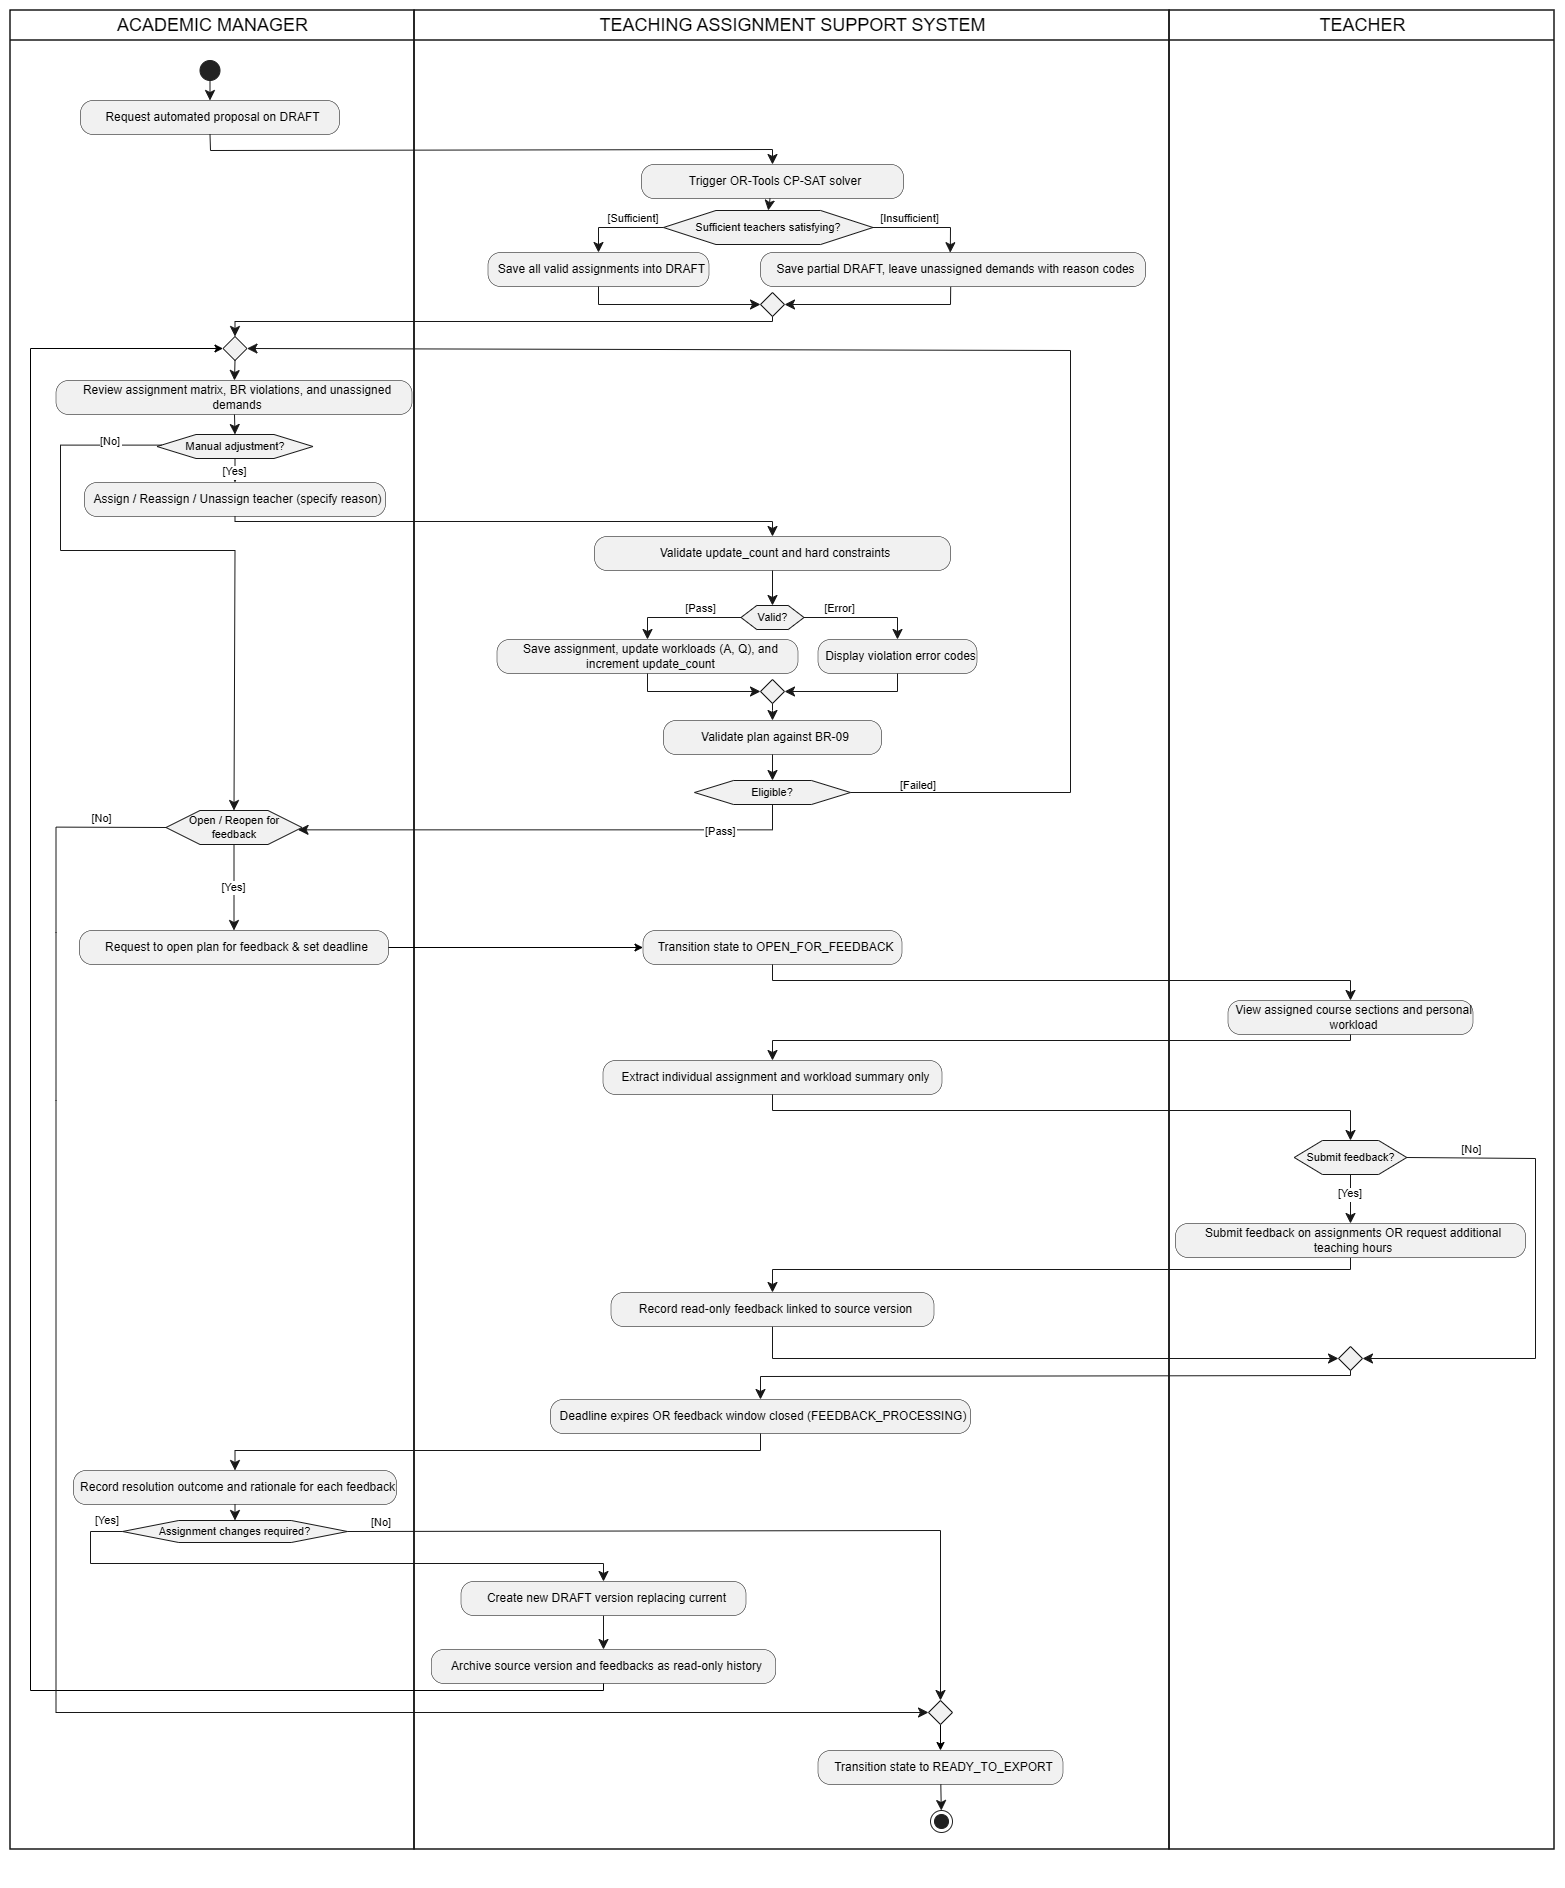
\includegraphics[width=0.98\linewidth,height=0.68\textheight,keepaspectratio]{diagrams/DG-04.png}
\caption{DG-04 --- Lập phương án và lấy phản hồi}\label{fig:DG-04}
\end{figure}

\diagramtext{Hai nhánh sau Solver đều lưu DRAFT: nhánh chưa phủ đủ giữ nhu cầu thiếu và lý do để người quản lý tiếp tục xử lý. Nhánh này chưa tự chứng minh thiếu giáo viên tối thiểu; mức bảo đảm phụ thuộc kết quả giải. Trước khi mở lấy ý kiến hoặc xuất, phương án phải qua BR-09. Nếu phản hồi làm đổi phân công, vòng xử lý tiếp tục trên DRAFT mới và giữ nguồn chỉ đọc theo FR-21.}



Hình~\ref{fig:DG-05} mô tả các trạng thái của phương án và những thao tác làm chuyển trạng thái. Sơ đồ dùng để xác định thời điểm được chỉnh sửa, nhận phản hồi và xuất tài liệu trong vòng đời ở bảng trên.

\begin{figure}[H]
\centering
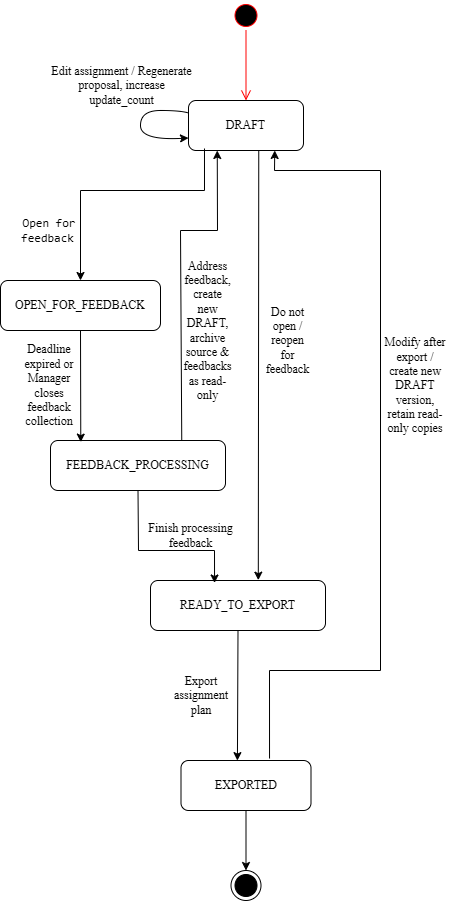
\includegraphics[width=0.98\linewidth,height=0.68\textheight,keepaspectratio]{diagrams/DG-05.png}
\caption{DG-05 --- Trạng thái phương án}\label{fig:DG-05}
\end{figure}

\diagramtext{Các cạnh quay về DRAFT sau phản hồi hoặc sau xuất được thực hiện bằng phiên bản mới theo BR-10; bản nguồn và tệp đã xuất vẫn được giữ. Đường từ DRAFT sang READY\_TO\_EXPORT chỉ áp dụng cho DRAFT sau phản hồi khi đủ điều kiện không mở lại tại FR-21. Nút kết thúc ở EXPORTED kết thúc một lượt xuất, không loại bỏ khả năng lập phiên bản tiếp theo.}


\chapter{YÊU CẦU HỆ THỐNG}\label{chap:functional}
Từ mô hình nghiệp vụ, chương này xác định các hành vi hệ thống phải cung cấp và cách kiểm chứng. Các bảng giữ mã yêu cầu để liên kết chức năng, Use Case, giao diện và tiêu chí chất lượng trong quá trình triển khai.


\section{Yêu cầu chức năng}

\begin{longtable}{|p{1.45cm}|p{12.5cm}|}
\hline
\textbf{ID} & \textbf{Yêu cầu và tiêu chí kiểm chứng} \\\hline
\endfirsthead
\hline
\textbf{ID} & \textbf{Yêu cầu và tiêu chí kiểm chứng} \\\hline
\endhead
FR-01 & \textbf{Đăng nhập và đăng xuất.} Với tài khoản hợp lệ, người dùng vào được hệ thống và nhận đúng vai trò; sau đăng xuất, phiên truy cập không còn dùng được. \\\hline
FR-02 & \textbf{Quản lý tài khoản và vai trò.} Administrator tạo, khóa/mở khóa tài khoản và gán một hoặc nhiều vai trò; người không có quyền bị từ chối và thao tác được ghi nhật ký. \\\hline
FR-03 & \textbf{Giới hạn truy cập theo vai trò và đơn vị.} Mỗi màn hình và thao tác kiểm tra cả quyền lẫn phạm vi dữ liệu; thử truy cập ngoài phạm vi phải bị từ chối. \\\hline
FR-04 & \textbf{Quản lý dữ liệu giáo viên và tổ chuyên môn.} Người có quyền thêm, xem, sửa, ngừng hiệu lực hồ sơ; mã giáo viên không trùng trong cùng phạm vi; dữ liệu đang được tham chiếu không bị xóa mất dấu vết. Nhiệm vụ GVCN không được lưu bằng cờ \texttt{isGVCN} trên hồ sơ giáo viên. \\\hline
FR-05 & \textbf{Quản lý môn học, khối lớp và lớp.} Người có quyền duy trì danh mục có mã duy nhất, trạng thái hiệu lực, quan hệ lớp--khối và môn--cấp học; mục hết hiệu lực không được chọn cho đợt mới. \\\hline
FR-06 & \textbf{Quản lý năng lực, kinh nghiệm và lịch sử giảng dạy.} Điều kiện năng lực lưu riêng cho từng giáo viên--môn--cấp học, trạng thái xác nhận, người/căn cứ xác nhận và hiệu lực để kiểm tra cứng theo BR-03. Không tự kế thừa năng lực từ cấp khác. Hồ sơ phân biệt chưa xác định/chưa có/đã có kinh nghiệm; khi đã có, nhập số năm theo môn và khối cùng mốc tính. Lưu lịch sử năm học, học kỳ, lớp, môn và thời gian thực tế đã dạy, kèm nguồn xác nhận; không cộng trùng số năm do dạy nhiều lớp đồng thời. Kinh nghiệm phục vụ BR-08, với trọng số cao hơn cho khối 9 và khối 12. \\\hline
FR-07 & \textbf{Cấu hình năm học, học kỳ và đợt phân công.} Mỗi đợt thuộc một học kỳ và có trạng thái; hệ thống không cho hai bản ghi trùng mã trong cùng đơn vị. \\\hline
FR-08 & \textbf{Quản lý phạm vi môn áp dụng và thành phần nhu cầu lớp--môn.} Academic Manager xác nhận môn--khối, trạng thái áp dụng và tập thành phần bắt buộc. Nhập STANDARD/SPECIALIZED\_TOPIC/ENRICHMENT cho từng lớp, số tiết dương với tối đa hai chữ số thập phân; đầu vào vượt độ chính xác bị từ chối trước khi ghi, không tự làm tròn. KHTN không tách mạch nội dung; không trùng thành phần/hiệu lực hoặc sửa lớp ngoài lựa chọn. Nhập nhiều lớp nguyên tử; đổi đầu vào làm kiểm tra cũ lỗi thời, bản đã mở lấy ý kiến hoặc xuất tài liệu giữ bản chụp dữ liệu, thay đổi qua DRAFT mới. \\\hline
FR-09 & \textbf{Quản lý định mức, nhiệm vụ kiêm nhiệm và giảm trừ.} Lưu loại nhiệm vụ, giáo viên, phạm vi, hiệu lực, mức giảm/quy đổi và nguồn bộ dữ liệu minh họa; GVCN gắn lớp. Phân biệt nhiệm vụ với chế độ đối tượng; tính lại tải theo bộ quy tắc có phiên bản tại Mục~\ref{sec:workload}. \\\hline
FR-12 & \textbf{Xem phân công và tải cá nhân.} Chỉ khi phiên bản hiện hành được mở lấy ý kiến, Teacher được xem lớp--môn--học kỳ, số tiết/tuần và tổng tải của chính mình; không được xem dữ liệu của giáo viên khác. \\\hline
FR-13 & \textbf{Quản lý phương án đang làm việc và lịch sử phiên bản.} Mỗi đợt chỉ có một phương án và một phiên bản hiện hành. Academic Manager khởi tạo phương án khi chưa có; thao tác tạo trùng bị từ chối. Phiên bản mới thay thế phiên bản hiện hành và lưu mã phiên bản nguồn, người tạo, thời điểm. Lịch sử chỉ đọc. Khôi phục một phiên bản cũ tạo DRAFT mới từ nội dung phiên bản đó và bắt buộc kiểm tra lại; không sửa bản cũ hoặc tạo nhánh phương án song song. \\\hline
FR-14 & \textbf{Chỉnh sửa phương án.} Academic Manager gán/đổi/bỏ gán trên DRAFT hiện hành; tối đa một giáo viên mỗi thành phần, cùng hoặc khác giáo viên theo BR-01. Gán thủ công/đã chốt có isLocked; chỉ Academic Manager mở khóa, lưu lý do và nhật ký. Bỏ gán có lý do. Lưu trong một giao dịch nguyên tử sau kiểm tra current\_version\_id, revision\_no, token và điều kiện cứng; xung đột không ghi đè, sửa lịch sử hoặc bỏ khóa. \\\hline
FR-15 & \textbf{Sinh đề xuất tự động (Must).} Ghi phiên bản đích, revision, InputSnapshot, RuleSetVersion, OptimizationConfig cho SolverRun. Tối ưu năm bước, giữ khóa và ngân sách theo Chương~\ref{chap:math-model}. Chỉ áp nghiệm khả thi đã hậu kiểm vào DRAFT còn đúng phiên bản, số lần cập nhật và mã kiểm soát dữ liệu đầu vào; lưu gán, lý do thiếu và tăng revision nguyên tử. Timeout có nghiệm khả thi tốt nhất đã tìm được hợp lệ vẫn được áp, bằng chứng tối ưu ghi riêng từng bước. Không nghiệm/lỗi/hủy/dữ liệu cũ giữ DRAFT. \\\hline
FR-16 & \textbf{Xem vi phạm và phần chưa phân công.} Với phương án đang làm việc, hệ thống hiển thị vi phạm/cảnh báo có mã BR, đối tượng và dữ liệu kiểm tra; liệt kê từng nhu cầu chưa gán cùng lý do sau sinh đề xuất hoặc chỉnh sửa. Lưu DRAFT một phần không đòi hỏi mọi nhu cầu đã được gán. \\\hline
FR-17 & \textbf{Tính tải giảng dạy.} Tính B, R, Q và A của đúng phiên bản; A khớp tổng số tiết các thành phần được gán. Hiển thị chính tổng công tác T=F+A+C+R, định mức B và chênh lệch T-B; đồng thời giữ F/C/W/R/Q, A-Q và W-Q để đối chiếu khi đủ dữ liệu, cùng đơn vị/kỳ tính và nguồn. Không cộng trùng tải cố định, lịch sử hoặc nguồn tải năm; thiếu dữ liệu không hiển thị như 0. Giới hạn pháp lý áp dụng biểu thức riêng theo quy tắc đã xác nhận. \\\hline
FR-18 & \textbf{Thống kê tải và tình trạng phân công.} Academic Manager xem thống kê tải theo giáo viên, tổ chuyên môn, môn hoặc khối của phương án hiện hành; nêu số nhu cầu đã/chưa phân công, vượt tải và thiếu tải. Không có màn hình so sánh các phương án song song. \\\hline
FR-19 & \textbf{Mở phương án cho phản hồi.} Chỉ DRAFT hiện hành đạt điều kiện mở tại BR-09 mới chuyển sang OPEN\_FOR\_FEEDBACK; lưu người mở, thời điểm, thời hạn và phiên bản được mở. Nếu kiểm tra năm chưa đủ dữ liệu, Academic Manager thấy rõ trạng thái và dữ liệu còn thiếu. Teacher chỉ xem phân công và tải cá nhân; đây không phải phê duyệt chính thức. \\\hline
FR-20 & \textbf{Gửi và theo dõi phản hồi cá nhân.} Teacher gửi phản hồi về gán cá nhân, tải cá nhân hoặc đề nghị nhận thêm tiết khi phiên bản hiện hành đang OPEN\_FOR\_FEEDBACK và còn hạn. Đề nghị chọn môn đang được gán và ghi tổng số tiết/tuần mong muốn của môn đó, lớn hơn tổng hiện tại trên phiên bản nguồn, cộng các lớp và thành phần đúng một lần. Đây là tổng mong muốn, không phải số tiết tăng thêm. Không tự tạo nhu cầu, sửa gán hoặc nới BR-06. Nội dung đã gửi giữ nguyên; trạng thái/kết quả xử lý được cập nhật theo quyền, và Teacher theo dõi được sau khi đóng/thay phiên bản. \\\hline
FR-21 & \textbf{Xử lý phản hồi và lập phiên bản kế tiếp.} Academic Manager ghi kết quả/lý do từng phản hồi, kể cả đề nghị nhận thêm tiết. Chấp nhận đề nghị chỉ dẫn đến chỉnh thủ công các nhu cầu đã có và kiểm tra lại điều kiện cứng; không tự tăng số tiết chương trình. Nếu không đổi phân công, phiên bản hiện hành có thể chuyển FEEDBACK\_PROCESSING sang READY\_TO\_EXPORT khi mọi phản hồi đã xử lý và đạt BR-09. Nếu đổi, tạo DRAFT mới thay hiện hành, giữ bản nguồn/phản hồi cũ chỉ đọc, kiểm tra lại và có thể mở lấy ý kiến lại. Nếu không mở lại, DRAFT mới chỉ sang READY\_TO\_EXPORT khi đạt BR-09, mọi phản hồi nguồn đã xử lý và quyết định không mở lại đã được ghi nhận. Không tạo phương án song song. \\\hline
FR-22 & \textbf{Xuất tài liệu phương án.} Academic Manager xuất PDF từ phiên bản hiện hành READY\_TO\_EXPORT đạt BR-09. PDF gồm hai góc nhìn theo giáo viên và theo lớp, có môn, loại thành phần, học kỳ, số tiết/tuần và bảng tải W/Q, T/B; ghi mã phương án/phiên bản, thời điểm, người xuất và nhãn Phương án đề xuất. Cảnh báo thiếu dữ liệu năm được in nổi bật cùng dữ liệu thiếu. Tạo/lưu tệp và kiểm tra lại phiên bản, số lần cập nhật và mã kiểm soát dữ liệu đầu vào trước khi ghi ExportRecord và EXPORTED; lỗi hoặc xung đột không phát hành thành công. Tải lại tệp đã lưu không phải tạo một lượt xuất mới từ EXPORTED. \\\hline
FR-23 & \textbf{Nhật ký thay đổi.} Người có quyền tra cứu thao tác quan trọng theo người dùng, thời điểm, đối tượng, hành động và giá trị trước/sau ở mức phù hợp. \\\hline
\end{longtable}


\section{Danh mục Use Case}\label{sec:usecases}
Các Use Case được phân loại theo mức độ ưu tiên: Must là yêu cầu bắt buộc, còn Should là yêu cầu khuyến nghị. Tất cả các UC trong bảng thuộc mức Must, ngoại trừ UC-21 thuộc mức Should. Quản trị, Quản lý và giáo viên lần lượt tương ứng với Administrator, Academic Manager và Teacher. Các yêu cầu FR liên quan quy định hành vi cần kiểm chứng.

\begin{longtable}{|p{1.25cm}|p{6.9cm}|p{2.6cm}|p{2.1cm}|}
\hline
\textbf{UC} & \textbf{Chức năng} & \textbf{Actor} & \textbf{FR} \\\hline
\endfirsthead
\hline
\textbf{UC} & \textbf{Chức năng} & \textbf{Actor} & \textbf{FR} \\\hline
\endhead
UC-01 & Đăng nhập hệ thống & Mọi vai trò & FR-01 \\\hline
UC-02 & Quản lý tài khoản và vai trò & Quản trị & FR-02--03 \\\hline
UC-03 & Quản lý dữ liệu giáo viên và tổ chuyên môn & Quản trị & FR-04 \\\hline
UC-04 & Quản lý môn học, khối lớp và lớp & Quản trị & FR-05 \\\hline
UC-05 & Quản lý năng lực, kinh nghiệm và lịch sử giảng dạy & Quản lý & FR-06 \\\hline
UC-06 & Thiết lập học kỳ và đợt phân công & Quản trị & FR-07 \\\hline
UC-07 & Chuẩn bị nhu cầu lớp--môn & Quản lý & FR-08 \\\hline
UC-08 & Cấu hình định mức và nhiệm vụ kiêm nhiệm & Quản trị, Quản lý & FR-09 \\\hline
UC-11 & Quản lý phương án đang làm việc và lịch sử phiên bản & Quản lý & FR-13 \\\hline
UC-12 & Chỉnh sửa phương án phân công & Quản lý & FR-14 \\\hline
UC-13 & Sinh đề xuất tự động & Quản lý & FR-15 \\\hline
UC-14 & Xem vi phạm và phần chưa phân công & Quản lý & FR-16 \\\hline
UC-15 & Thống kê tải và tình trạng phân công & Quản lý & FR-17--18 \\\hline
UC-16 & Mở phương án cho phản hồi & Quản lý & FR-19 \\\hline
UC-17 & Xem phân công và tải cá nhân & giáo viên & FR-12 \\\hline
UC-18 & Gửi và theo dõi phản hồi cá nhân & giáo viên & FR-20 \\\hline
UC-19 & Xử lý phản hồi và lập phiên bản kế tiếp & Quản lý & FR-21 \\\hline
UC-20 & Xuất tài liệu phương án & Quản lý & FR-22 \\\hline
UC-21 & Tra cứu nhật ký & Quản trị & FR-23 \\\hline
\end{longtable}


Các Use Case trong bảng được tổ chức theo vai trò và nhóm nghiệp vụ tại Hình~\ref{fig:DG-02}. Sơ đồ giúp đối chiếu phạm vi tương tác của người dùng với các nhóm quản trị dữ liệu, lập/kiểm tra phương án và phản hồi/xuất tài liệu.

\begin{figure}[H]
\centering
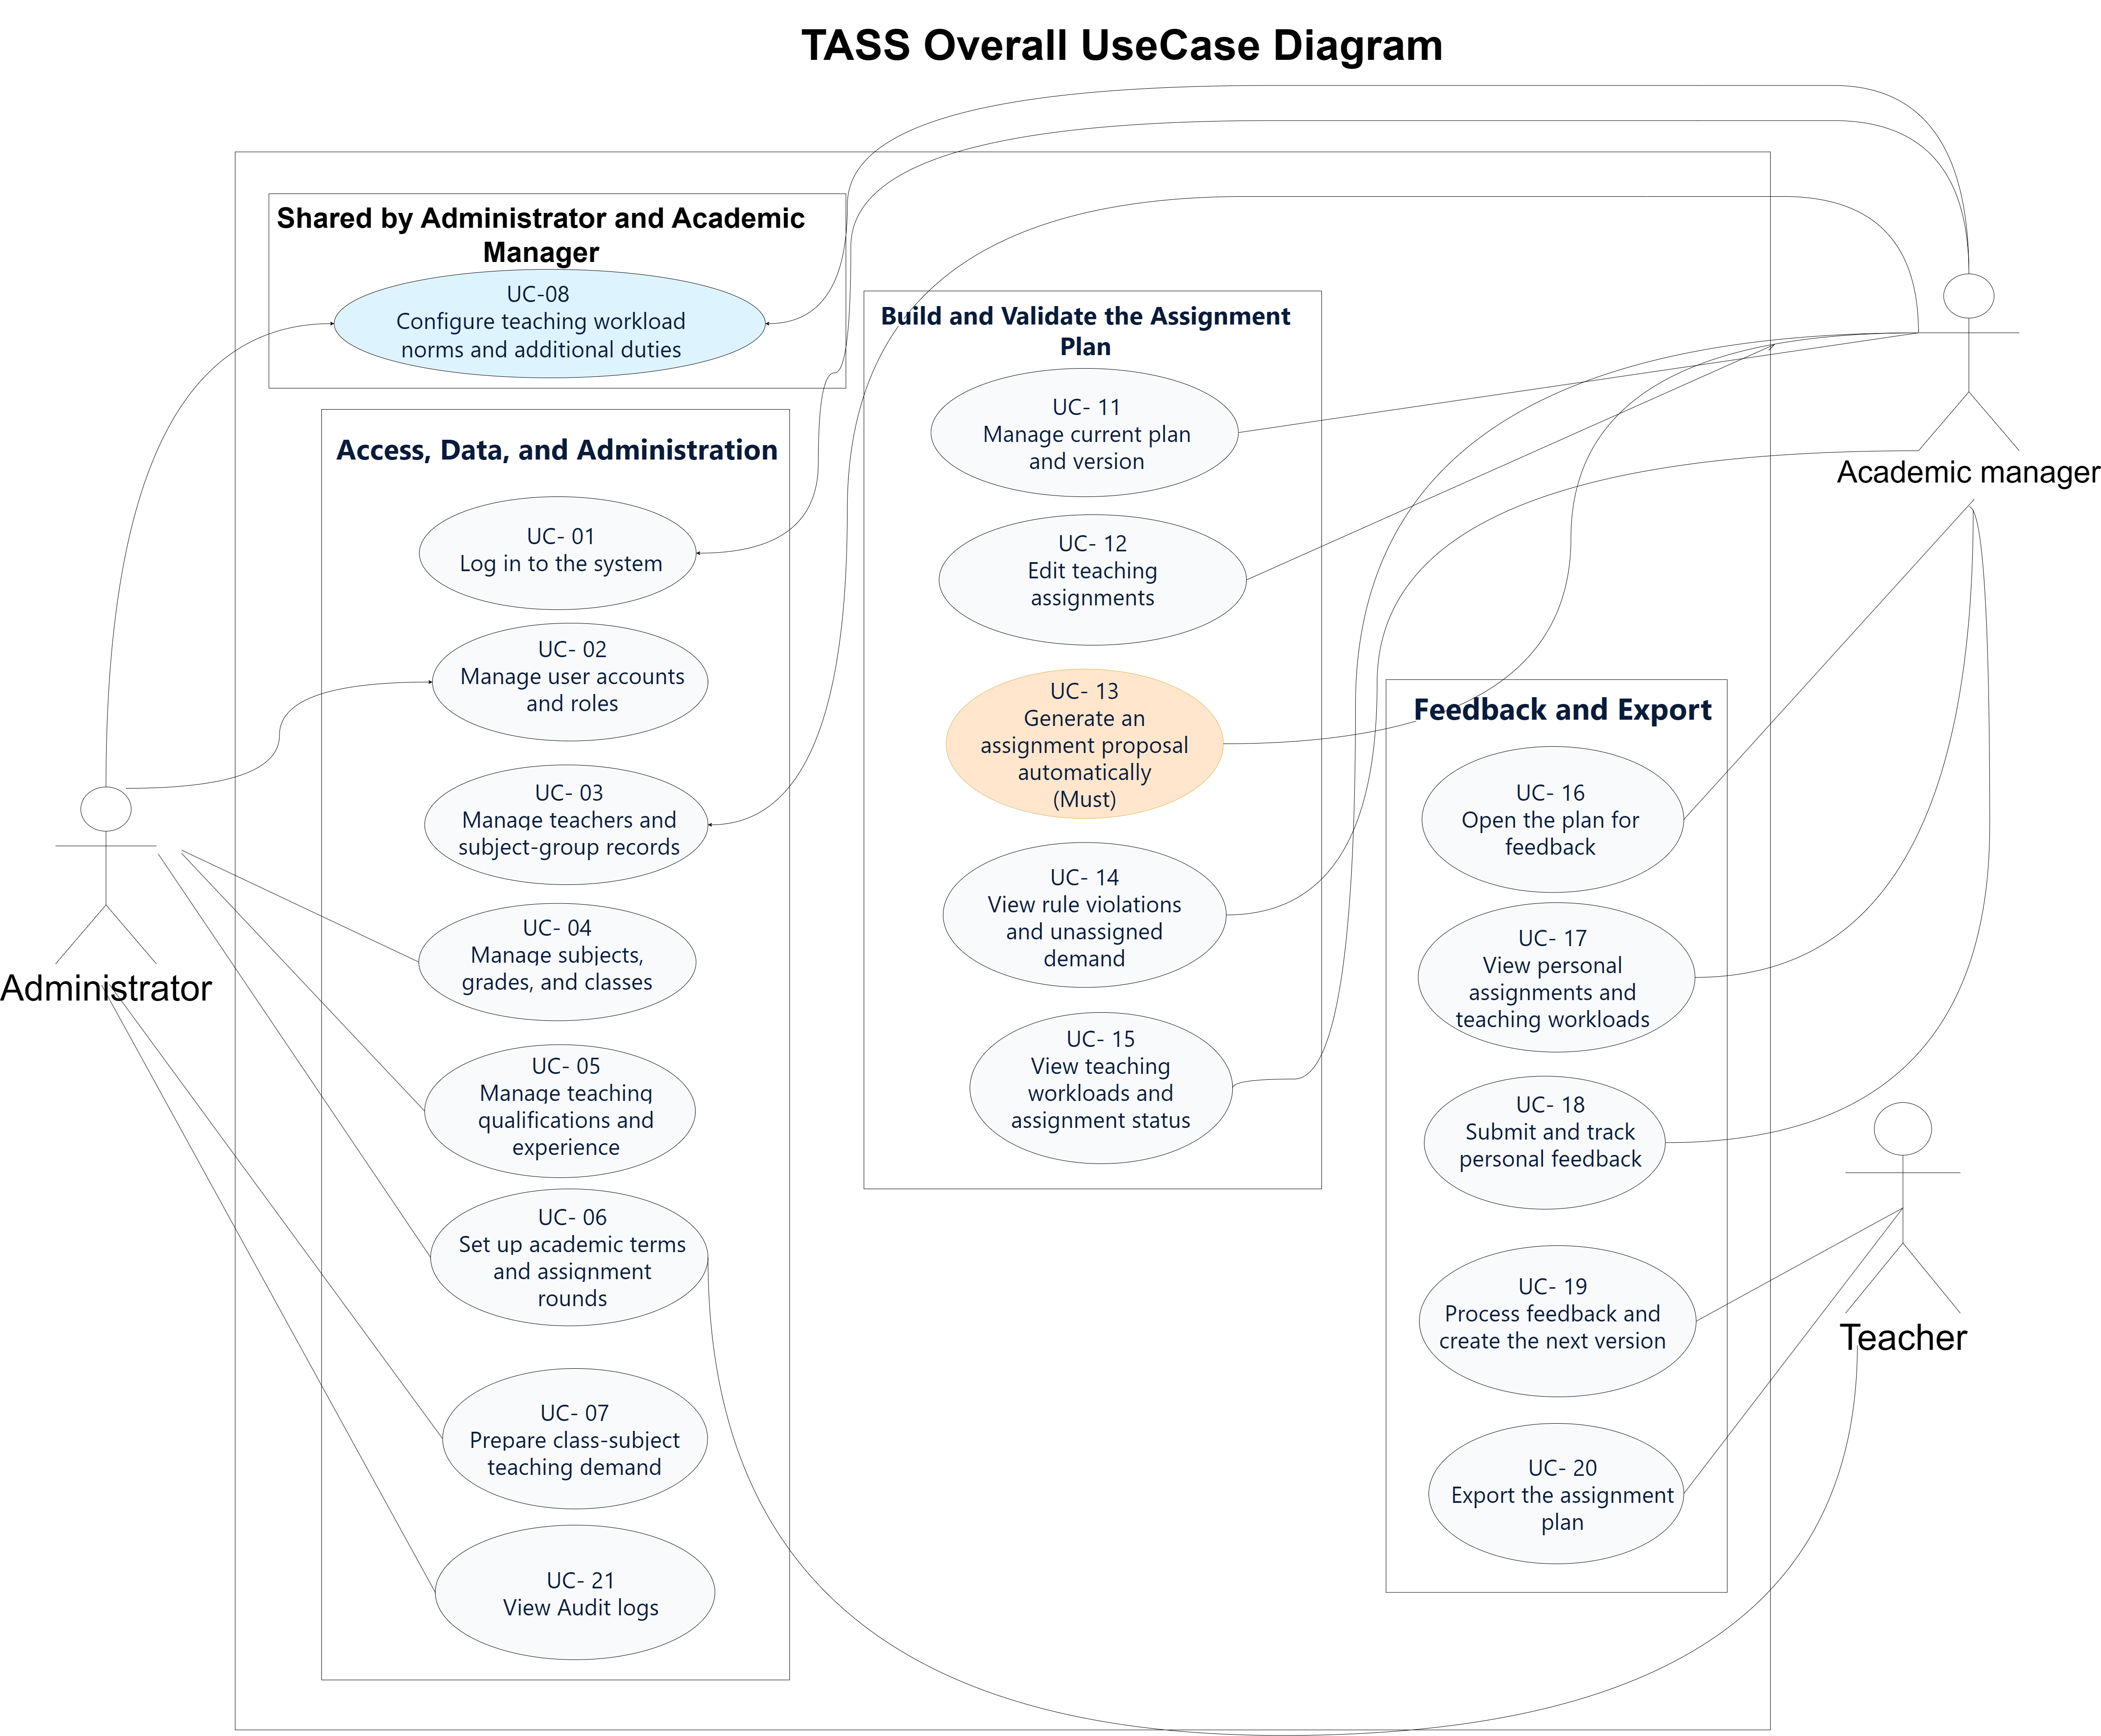
\includegraphics[width=0.98\linewidth,height=0.70\textheight,keepaspectratio]{diagrams/DG-02.png}
\caption{DG-02 --- Use Case tổng quát}\label{fig:DG-02}
\end{figure}

\diagramtext{UC-13 ở nhóm lập phương án thể hiện chức năng sinh đề xuất tự động bắt buộc; UC-08 là chức năng dùng chung theo quyền. Teacher tham gia xem và phản hồi cá nhân qua UC-17/18 cùng chức năng đăng nhập. Quyền thực thi từng UC căn cứ bảng Use Case và FR-03; sơ đồ thể hiện quan hệ actor--chức năng, còn thứ tự xử lý được mô tả ở DG-03/04.}


\section{Giao diện và tích hợp}\label{sec:interfaces}

\begin{longtable}{|p{1.45cm}|p{12.5cm}|}
\hline
\textbf{ID} & \textbf{Giao diện và yêu cầu} \\\hline
\endfirsthead
\hline
\textbf{ID} & \textbf{Giao diện và yêu cầu} \\\hline
\endhead
IF-01 & \textbf{Đăng nhập.} Hiển thị lỗi không tiết lộ tài khoản có tồn tại; hỗ trợ đăng xuất rõ ràng. \\\hline
IF-02 & \textbf{Danh mục.} Có tìm kiếm, lọc trạng thái, phân trang khi cần và xác nhận trước thao tác ảnh hưởng dữ liệu. \\\hline
IF-03 & \textbf{Chuẩn bị dữ liệu đợt.} Hiển thị danh sách môn--khối đã xác nhận và số cặp lớp--môn áp dụng, không áp dụng, chưa xác định hoặc áp dụng nhưng thiếu số tiết; chỉ báo sẵn sàng khi dữ liệu bắt buộc trong phạm vi đã xác nhận đầy đủ. \\\hline
IF-04 & \textbf{Bảng phân công.} Hiển thị một phương án hiện hành của đợt, có thao tác sinh đề xuất tự động và chỉnh gán trong DRAFT. Lịch sử phiên bản chỉ đọc; không có tạo nhánh hoặc so sánh phương án song song, không có trục thứ/buổi/tiết. \\\hline
IF-05 & \textbf{Bảng tải.} Hiển thị chính Tổng tiết T / Tiết định mức B / Lệch tải T-B; đối chiếu A/F/C/W/R/Q khi đủ dữ liệu, có đơn vị/kỳ/nguồn. Giá trị chưa biết không thành 0. Teacher chỉ xem cá nhân theo trạng thái được phép. \\\hline
IF-06 & \textbf{Vi phạm và phần chưa phân công.} Phân biệt cứng/mềm bằng nhãn, liên kết tới đối tượng cần sửa; luôn hiển thị nhu cầu chưa gán và lý do trong DRAFT một phần, không coi thiếu giáo viên là lỗi làm mất phương án. \\\hline
IF-07 & \textbf{Mở và xử lý phản hồi.} Academic Manager mở phiên bản hiện hành, xem thời hạn, danh sách/trạng thái phản hồi và kết quả xử lý. Thao tác lập phiên bản kế tiếp thay thế bản hiện hành, giữ bản nguồn và phản hồi chỉ đọc; không tạo phương án song song. \\\hline
IF-08 & \textbf{Cổng giáo viên.} Khi mở lấy ý kiến, chỉ hiển thị phân công và tải cá nhân, cho phản hồi về gán, tải cá nhân hoặc đề nghị nhận thêm tiết của môn đang dạy trong hạn; cho theo dõi kết quả phản hồi cá nhân sau khi đóng. Đề nghị chỉ gửi người quản lý; không có đăng ký môn/khối muốn dạy, khai lịch bận hoặc sửa phương án. \\\hline
IF-09 & \textbf{Biểu mẫu nhập và xuất PDF.} Chọn môn--khối, lớp và trạng thái áp dụng; xác nhận loại thành phần bắt buộc trước khi nhập. Cho nhập nhóm hoặc sửa riêng theo lớp--môn--loại, số tiết dương theo độ chính xác đã xác nhận; lỗi đúng lớp/trường, không đổi lớp ngoài lựa chọn. Màn hình xuất hiển thị phiên bản/revision và tải PDF có loại thành phần, mã phiên bản, thời điểm; tải lại tệp phát hành giữ nguyên nội dung. \\\hline
\end{longtable}

Dữ liệu sản phẩm nhập qua biểu mẫu, xuất PDF theo FR-22. JSON bộ dữ liệu kiểm thử dùng test Solver, không phải import Excel. Tích hợp bổ sung cần hợp đồng dữ liệu, xác thực, phiên bản và xử lý lỗi riêng.

\section{Yêu cầu phi chức năng}\label{sec:nfr}
Các ngưỡng dưới đây là mục tiêu cần được kiểm chứng, chưa phải kết quả đã đạt. Những tham số về bảo mật và vận hành được lưu theo cấu hình của từng bản phát hành.

\begin{longtable}{|p{1.45cm}|p{12.5cm}|}
\hline
\textbf{ID} & \textbf{Yêu cầu và cách đo} \\\hline
\endfirsthead
\hline
\textbf{ID} & \textbf{Yêu cầu và cách đo} \\\hline
\endhead
NFR-01 & 95\% yêu cầu danh sách/hồ sơ/bảng tải phản hồi tối đa 2 giây. \textit{Kiểm chứng:} Đo từ máy chủ nhận yêu cầu đến trả phản hồi; ghi bản chụp dữ liệu, tải thử và cấu hình máy. \\\hline
NFR-02 & 95\% lượt kiểm tra lại ràng buộc phương án hoàn tất tối đa 5 giây. \textit{Kiểm chứng:} Đo trên dữ liệu/cấu hình chuẩn, ghi phạm vi tiền/hậu kiểm. \\\hline
NFR-03 & Sinh đề xuất Must: toàn lượt kết thúc bằng kết quả/trạng thái cuối trong mục tiêu 60 giây trên bản chụp dữ liệu E3/cấu hình chuẩn; chấp nhận DRAFT một phần hợp lệ. \textit{Kiểm chứng:} Đo gồm thời gian chờ, bản chụp dữ liệu, tiền kiểm, Solver, hậu kiểm và áp dụng. Thử đủ/thiếu/căng tải, timeout/lỗi và dữ liệu đổi; không ghi đè bằng kết quả cũ. \\\hline
NFR-04 & Mọi lưu DRAFT, thay phiên bản và chuyển trạng thái kiểm tra trong cùng giao dịch phiên bản, số lần cập nhật và mã kiểm soát dữ liệu đầu vào; gán/lý do/tăng revision trong một giao dịch, lịch sử chỉ đọc. \textit{Kiểm chứng:} Hai tab cùng revision: một lưu thành công, yêu cầu cũ bị từ chối. Thử tạo phiên bản đồng thời, DRAFT thiếu và lỗi giao dịch; không phát sinh nhánh/lưu dở. \\\hline
NFR-05 & Mọi kết nối có thông tin xác thực hoặc dữ liệu cá nhân phải được mã hóa khi truyền; mật khẩu phải được băm bằng cơ chế phù hợp của nền tảng. \textit{Kiểm chứng:} Rà soát cấu hình và thử truy cập qua kênh không an toàn. \\\hline
NFR-06 & Đăng nhập, phân quyền, đổi quy tắc, sinh đề xuất, sửa phương án, xử lý phản hồi và thay phiên bản hiện hành phải có nhật ký không cho người dùng thường sửa. \textit{Kiểm chứng:} Đối chiếu thao tác với nhật ký, phiên bản nguồn và phản hồi để bảo đảm truy vết sau khi cập nhật. \\\hline
NFR-07 & Phiên đăng nhập hết hiệu lực sau khoảng không hoạt động cấu hình. \textit{Kiểm chứng:} Thử hết phiên và đăng nhập lại theo cấu hình bảo mật. \\\hline
NFR-08 & Sao lưu/khôi phục đáp ứng RPO, RTO và lịch lưu trữ được cấu hình trước vận hành. \textit{Kiểm chứng:} Khôi phục bản sao, đo thời gian và điểm dữ liệu khôi phục. \\\hline
NFR-09 & Luồng Must dùng bằng bàn phím; trường có nhãn, lỗi/cảnh báo không chỉ dùng màu. \textit{Kiểm chứng:} Thử các UC Must và công cụ hỗ trợ truy cập của bản phát hành. \\\hline
NFR-10 & Giao diện web dùng được từ chiều rộng 1280 pixel trên trình duyệt mục tiêu. \textit{Kiểm chứng:} Kiểm tra danh sách trình duyệt/phiên bản công bố cùng cấu hình triển khai. \\\hline
NFR-11 & Khi lưu biểu mẫu lỗi hoặc bị gián đoạn, không làm mất dữ liệu hợp lệ đã lưu và chỉ rõ lớp/trường cần sửa. \textit{Kiểm chứng:} Thử trạng thái áp dụng thiếu, cặp áp dụng thiếu thành phần bắt buộc/số tiết, số tiết không dương/sai độ chính xác, trùng loại, lớp ngoài khối, phản hồi quá hạn và gián đoạn lưu nhóm; giao dịch nhóm nguyên tử. \\\hline
NFR-12 & Mỗi bản phát hành phải có kiểm thử tự động cho quy tắc cứng và các chuyển trạng thái phương án. \textit{Kiểm chứng:} Báo cáo kiểm thử phải ghi phiên bản mã nguồn, bộ dữ liệu và kết quả của từng ca thử. \\\hline
NFR-13 & Mã nguồn và cấu hình tách biệt; bí mật không được lưu trực tiếp trong kho mã. \textit{Kiểm chứng:} Rà soát kho mã và quy trình cấu hình triển khai. \\\hline
NFR-14 & PDF có tiêu đề, phạm vi, loại thành phần, học kỳ, đơn vị tải, mã phương án/phiên bản, thời điểm và nhãn Phương án đề xuất. Cùng payload bản chụp dữ liệu và cấu hình thì các dòng/số liệu nhất quán; không yêu cầu đồng nhất từng byte. \textit{Kiểm chứng:} Kiểm tra bộ tạo PDF hai lần trên cùng dữ liệu đóng băng trong môi trường kiểm thử, hoặc đối chiếu tải lại tệp đã lưu. Đây không phải quyền tạo lượt xuất mới từ EXPORTED; chỉ tải lại tệp đã phát hành theo FR-22. \\\hline
\end{longtable}


\chapter{THIẾT KẾ DỮ LIỆU VÀ KIẾN TRÚC}\label{chap:data}
Thiết kế dữ liệu phải lưu được nhu cầu giảng dạy, điều kiện của giáo viên và toàn bộ lịch sử xử lý phương án. Chương này tổ chức các yêu cầu đó thành mô hình dữ liệu, trình bày cách chuẩn hóa nguồn Excel và mô tả kiến trúc triển khai dự kiến.


\section{Mô hình dữ liệu}\label{sec:data-model}

\begin{longtable}{|p{1.45cm}|p{12.5cm}|}
\hline
\textbf{ID} & \textbf{Đối tượng và dữ liệu cần lưu} \\\hline
\endfirsthead
\hline
\textbf{ID} & \textbf{Đối tượng và dữ liệu cần lưu} \\\hline
\endhead
DATA-01 & \textbf{Người dùng và quyền.} Mã người dùng, trạng thái, vai trò, phạm vi đơn vị; thông tin xác thực không lưu dạng rõ. \\\hline
DATA-02 & \textbf{Giáo viên và công tác học kỳ.} Teacher giữ định danh/họ tên; TeacherEmployment lưu giáo viên, tổ, học kỳ, trạng thái công tác, chức danh và hiệu lực. Không có hai khoảng công tác chồng nhau cho cùng giáo viên--học kỳ theo thiết kế này. Phân biệt nghỉ thai sản với chế độ nuôi con. Không dùng cờ isGVCN; GVCN lưu ở TeacherDuty gắn lớp. \\\hline
DATA-03 & \textbf{Chuyên môn, kinh nghiệm và lịch sử.} Năng lực xác nhận theo giáo viên--môn--cấp học, với người/căn cứ xác nhận và hiệu lực; KHTN dùng năng lực toàn môn. Kinh nghiệm lưu theo giáo viên--môn--khối, trạng thái đã/chưa có hoặc chưa xác định, số năm dạng số không âm, mốc tính, nguồn và người/thời điểm xác nhận; số năm bằng 0 khác với dữ liệu chưa biết. TeachingHistory lưu năm học/học kỳ, lớp, môn và khoảng thực tế đã dạy, có thể bổ sung từ trước khi sử dụng hệ thống. Không coi mọi DRAFT/phương án đề xuất là kinh nghiệm đã thực hiện, không cộng trùng thời gian dạy nhiều lớp. Điểm phạt tính theo DATA-13 và được giữ trong snapshot. \\\hline
DATA-04 & \textbf{Lớp, môn và phạm vi áp dụng.} Danh mục xác định lớp, khối, cấp học và môn; KHTN có một mã môn, không cần quan hệ môn cha/phân môn trong demo. RoundSubjectScope ghi phạm vi môn và khối của đợt; ClassSubjectApplicability lưu trạng thái áp dụng, lý do và thông tin xác nhận cho từng cặp lớp--môn. Tập thành phần bắt buộc phải liên kết được với nhu cầu đáp ứng tương ứng, thay vì dùng một demand\_id cho cả cặp lớp--môn. RequiredDemandComponent lưu loại, hiệu lực, liên kết nhu cầu và thông tin xác nhận; ClassSubjectApplicability lưu xác nhận riêng cho toàn bộ tập thành phần bắt buộc. SourceImport cùng TeacherAlias, ClassAlias và SubjectAlias ánh xạ bí danh tới ID bất biến, giữ tệp, sheet, ô, giá trị gốc và thông tin xác nhận. \\\hline
DATA-05 & \textbf{Học kỳ và đợt.} Năm học, học kỳ, đơn vị, thời hạn, trạng thái, bộ quy tắc áp dụng và tham chiếu duy nhất tới phương án đang làm việc của đợt. \\\hline
DATA-06 & \textbf{Thành phần nhu cầu lớp--môn.} TeachingDemand có ID, class\_id bắt buộc, môn, học kỳ, loại, số tiết dương với tối đa hai chữ số thập phân, đơn vị và hiệu lực. Khóa nghiệp vụ theo lớp--môn--kỳ--loại--giai đoạn; không có group\_id hoặc bảng thành viên trong demo. Ba loại thành phần lưu riêng; mỗi thành phần bắt buộc liên kết được với nhu cầu đáp ứng. Nhu cầu chương trình KHTN lưu toàn môn, không tạo thêm các nhu cầu Lý/Hóa/Sinh. Nhập nhiều lớp được thực hiện nguyên tử. \\\hline
DATA-07 & \textbf{Định mức, nhiệm vụ và chế độ giảm trừ.} TeacherWorkloadBasis lưu định mức cơ sở theo hồ sơ cấp công tác THCS/THPT, chức danh, đơn vị, hiệu lực, nguồn và thông tin xác nhận; các khoảng của cùng giáo viên--học kỳ không chồng nhau. TeacherDuty có loại, giáo viên, phạm vi, thời hạn, giá trị và nguồn; GVCN gắn lớp. Dùng bộ dữ liệu minh họa Mục~\ref{sec:workload}; metadata chế độ đối tượng giữ riêng, chưa kích hoạt chế độ đặc thù/thẩm định đầy đủ chi trả. \\\hline
DATA-09 & \textbf{Phương án và lịch sử phiên bản.} AssignmentPlan duy nhất theo round\_id, current\_version\_id thuộc chính plan. PlanVersion có version\_no, source\_version\_id, revision\_no, trạng thái, hạn phản hồi và InputSnapshot. PlanDemand duy nhất theo phiên bản--nhu cầu, giữ số tiết bản chụp dữ liệu, isLocked, người/thời điểm/lý do khóa; khóa phải có giáo viên hợp lệ; teacher\_id NULL phải có mã/nội dung lý do. Snapshot bất biến chứa đủ danh mục, phạm vi, thành phần, năng lực/công tác, tải, quy tắc và cấu hình để xem lại không lệ thuộc dữ liệu sống. Phiên bản bị thay thế chỉ đọc, không sửa hồi tố hoặc tạo nhánh song song. \\\hline
DATA-10 & \textbf{Kết quả kiểm tra.} ValidationRun gắn phiên bản, revision\_no, InputSnapshot và thời điểm. ValidationResult ghi mã BR, đối tượng, kỳ tính, PASS, VIOLATION hoặc INSUFFICIENT\_DATA, mức độ, dữ liệu thiếu và thông báo. Chỉ kết quả cùng phiên bản, số lần cập nhật và mã kiểm soát dữ liệu đầu vào mới được dùng cho mở lấy ý kiến hoặc xuất tài liệu. Thiếu dữ liệu năm không biến thành PASS; thay đổi dữ liệu làm kết quả cũ không còn quyền cho phép thao tác. \\\hline
DATA-11 & \textbf{Nhật ký.} Người thực hiện, thời điểm, hành động, đối tượng, kết quả và dữ liệu trước/sau phù hợp. \\\hline
DATA-12 & \textbf{Phản hồi phân công.} Lưu giáo viên gửi, phiên bản nguồn, loại phản hồi (gán cá nhân, tải cá nhân, đề nghị nhận thêm tiết), nội dung, thời điểm, trạng thái/kết quả, người xử lý và phiên bản kế tiếp nếu có. plan\_demand\_id tùy chọn nhưng phải đúng giáo viên và phiên bản nguồn. Đề nghị nhận thêm tiết lưu môn đang được gán và requested\_periods\_per\_week là tổng mong muốn của môn, không phải phần tăng; tổng nguồn lấy từ bản chụp dữ liệu các thành phần. Nội dung bất biến sau gửi; trạng thái/kết quả được người có quyền xử lý trước khi đóng lịch sử. \\\hline
DATA-13 & \textbf{Cấu hình tối ưu.} OptimizationConfig có phiên bản, thứ tự Z/L1/M/experience/change, cơ sở T-B, khóa, giới hạn thời gian tổng thể và của từng bước. Lưu quy tắc chuyển số năm kinh nghiệm theo môn/khối tại mốc tính thành điểm phạt, trọng số khối cuối cấp và các khối còn lại, cùng $\beta=1$ cho bước kinh nghiệm độc lập. Trọng số khối 9 và 12 lớn hơn trọng số các khối khác; điểm phạt mềm tách hệ số quy đổi pháp lý. Ghi chính sách BR-01 trong cấu hình. \\\hline
DATA-14 & \textbf{Bộ quy tắc có căn cứ.} Mã văn bản, điều/khoản/điểm, thời gian hiệu lực, loại cơ sở, cấp học, chức danh, vùng, ngưỡng lớp, mức/đơn vị và điều kiện áp dụng; bản nguồn, người xác nhận và phiên bản quy tắc. Phương án lưu phiên bản được sử dụng. \\\hline
DATA-15 & \textbf{Bối cảnh trường và quỹ giảm trừ.} Loại trường, vùng, số lớp, tình trạng vị trí và quỹ giáo vụ/tư vấn lưu phục vụ mở rộng; chưa kích hoạt tính quỹ BR-20 trong MVP. \\\hline
DATA-16 & \textbf{Kỳ tính và tải năm học.} Số tuần giảng dạy thực tế/kế hoạch theo giai đoạn, tải đã thực hiện ngoài phương án, định mức và phần vượt theo tuần/năm. Bộ E3 2026--2027 dùng HK1 18/HK2 17 tuần; năm khác cấu hình riêng. Không tính trùng các phiên bản.  \\\hline
DATA-17 & \textbf{Hoạt động được quy đổi.} Giáo viên, hoạt động, số tiết thực tế, đơn vị gốc, kỳ tính, hệ số cố định/trần, hệ số được quyết định, số tiết quy đổi, nguồn điều/khoản và chứng cứ. Quyết định là đầu vào ngoài hệ thống.  \\\hline
DATA-18 & \textbf{Lượt sinh đề xuất.} SolverRun gắn plan\_version\_id, base\_revision\_no, input\_snapshot\_id, người yêu cầu và thời gian; result\_summary\_json lưu phiên bản OR-Tools, cấu hình, seed, số worker, ngân sách, trạng thái, giá trị hàm mục tiêu và cận biên (status/objective/bound) của từng bước Z/L1/M/experience/change, độ phủ và kết quả áp dụng. applied\_revision\_no chỉ có khi lưu thành công. Tách trạng thái CP-SAT, nguyên nhân kết thúc và kết quả áp dụng; kết quả hết thời gian nhưng khả thi có thể áp dụng nếu còn mới. \\\hline
\end{longtable}

InputSnapshot lưu bản chụp đầy đủ của dữ liệu hiển thị, phạm vi, thành phần nhu cầu, công tác, năng lực, kinh nghiệm và điểm phạt, tải, quy tắc và cấu hình, thay vì chỉ lưu ID trỏ tới dữ liệu đang thay đổi. ValidationRun gắn với phiên bản, số lần cập nhật, bản chụp và mã kiểm soát dữ liệu đầu vào để xác định kết quả kiểm tra còn hiệu lực. Các mã nghiệp vụ phải duy nhất; việc cập nhật hiệu lực phải bảo toàn lịch sử, còn thao tác nhập theo nhóm phải được thực hiện trong một giao dịch. Hệ thống chỉ thu thập dữ liệu cá nhân cần thiết cho phân công [17]--[19] và áp dụng quy trình lưu trữ, xóa hoặc ẩn danh theo cấu hình vận hành.

Hình~\ref{fig:DG-06} tổ chức các yêu cầu DATA thành mô hình miền, làm rõ đối tượng nghiệp vụ và liên hệ giữa chúng trước khi thiết kế bảng dữ liệu. Có thể đọc từ học kỳ/đợt, qua phạm vi môn và nhu cầu, đến phương án, phiên bản và từng gán giáo viên.

\begin{figure}[H]
\centering
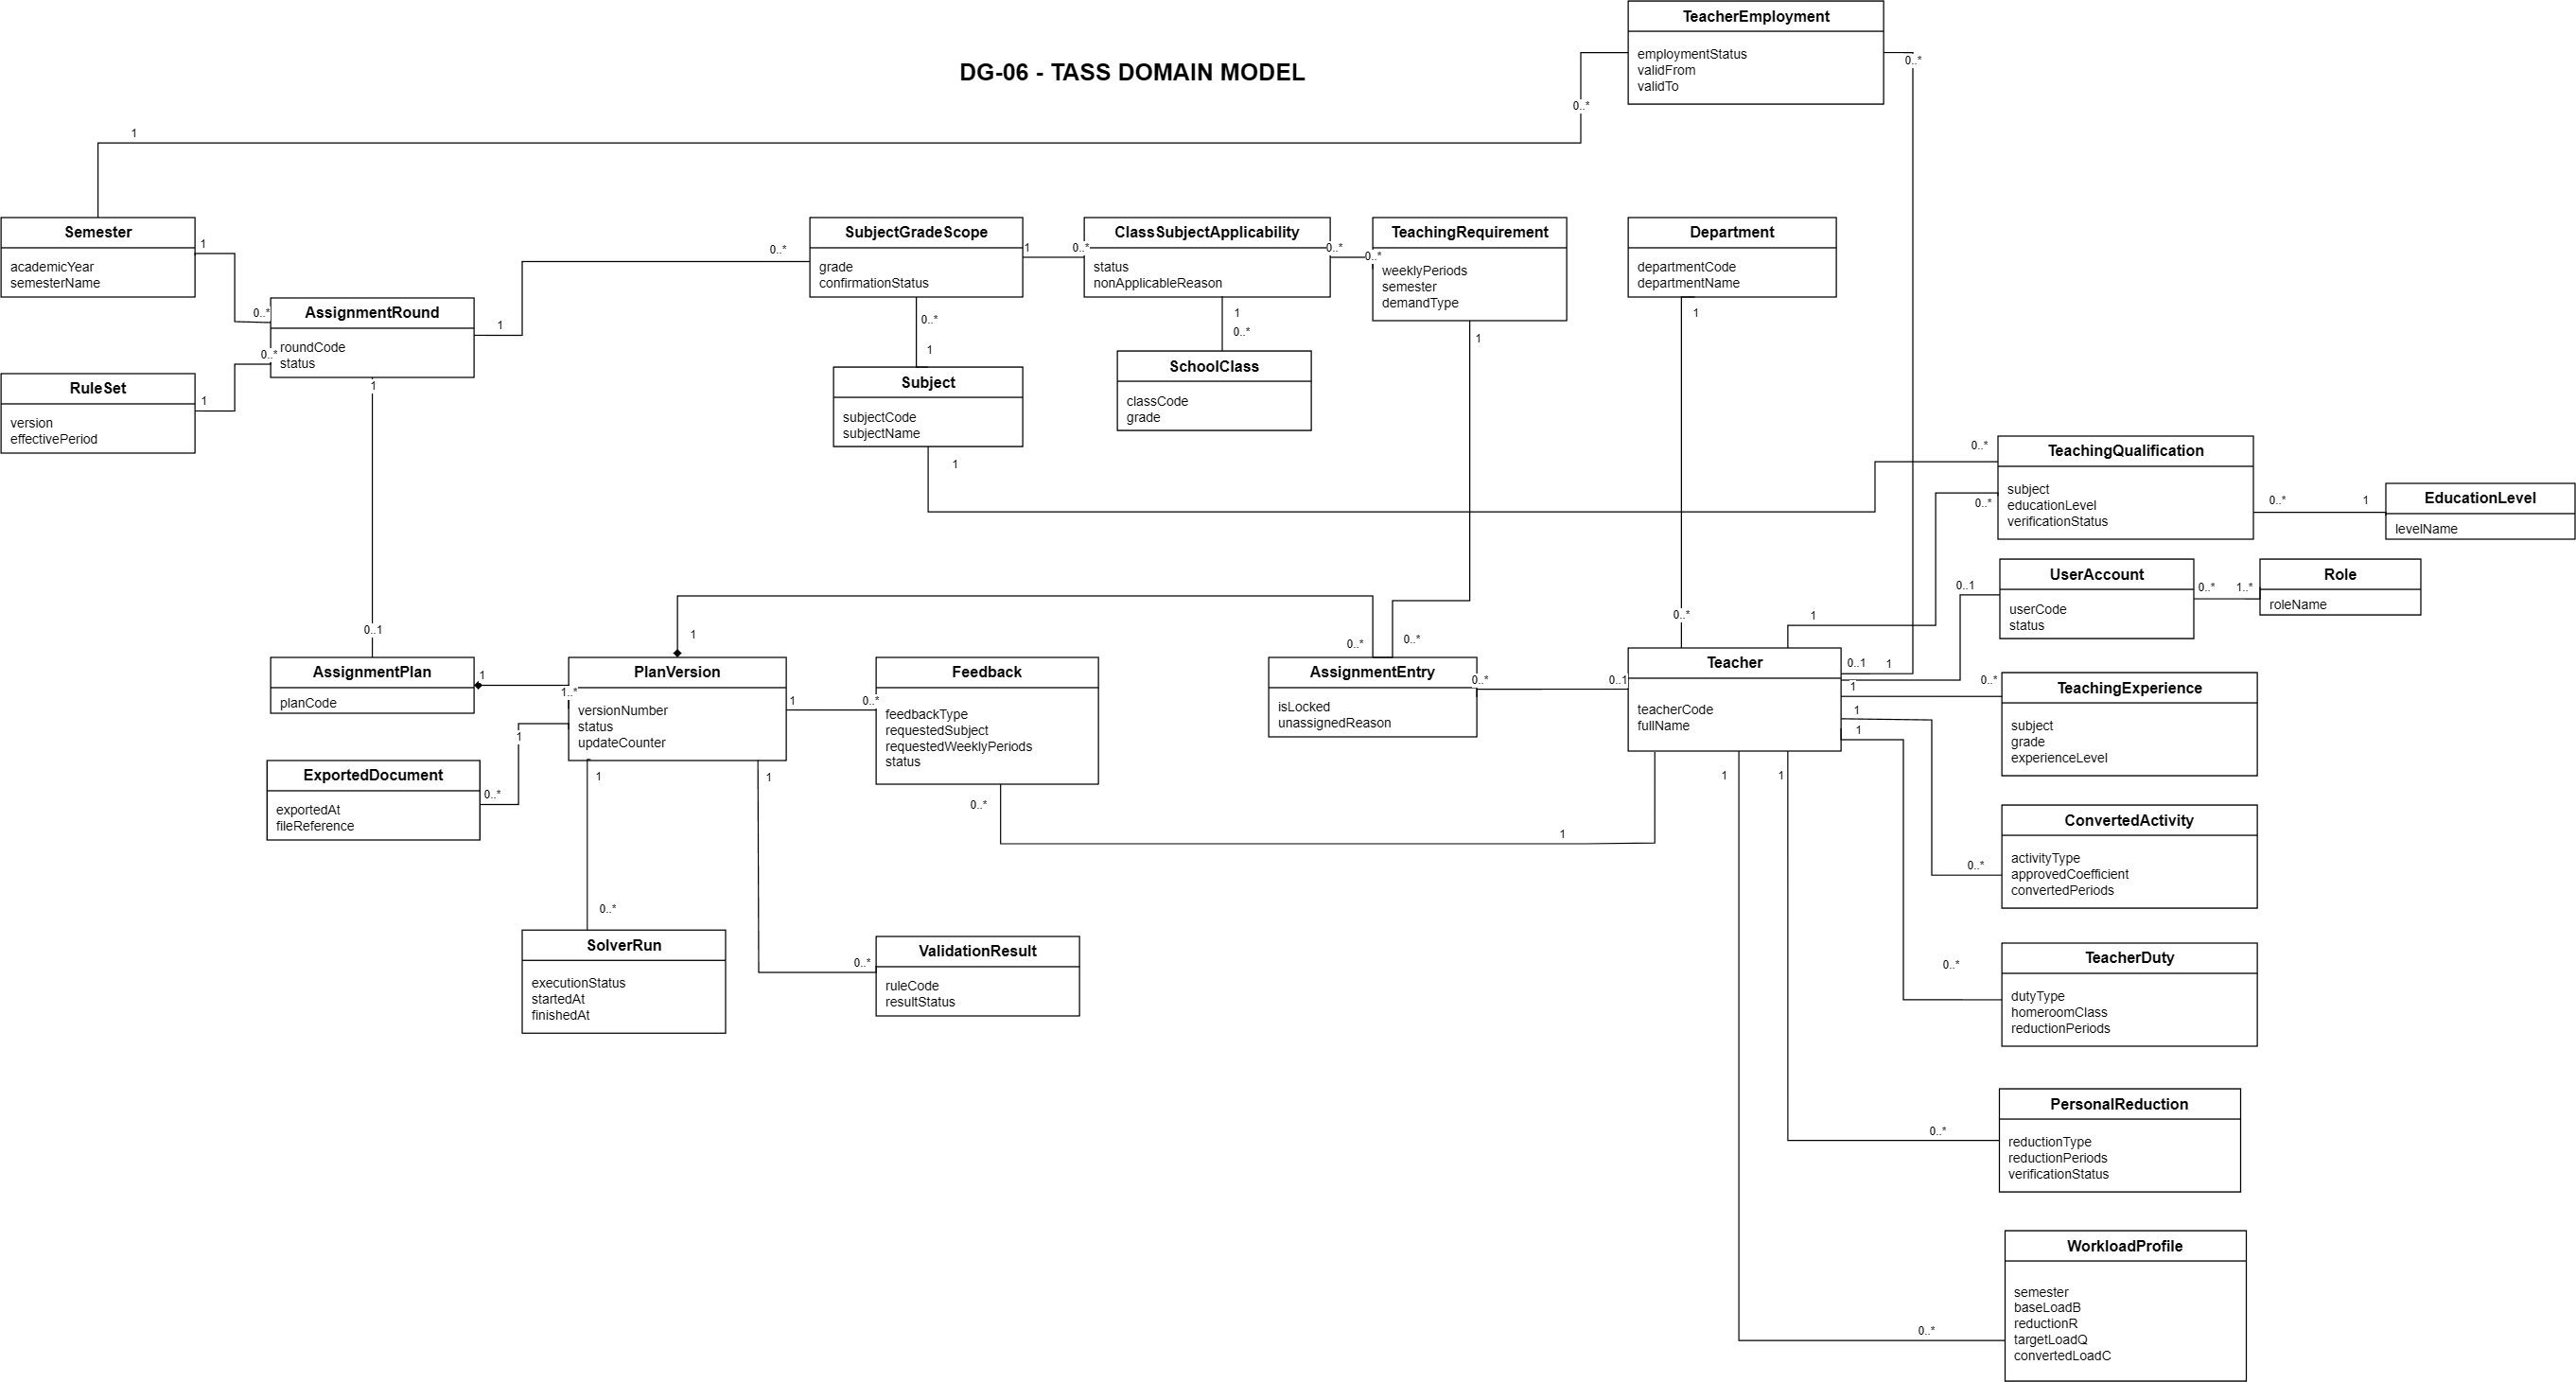
\includegraphics[width=0.98\linewidth,height=0.47\textheight,keepaspectratio]{diagrams/DG-06.png}
\caption{DG-06 --- Mô hình miền}\label{fig:DG-06}
\end{figure}

\diagramtext{Nhóm hồ sơ giáo viên, công tác và chuyên môn cung cấp điều kiện ứng viên; kinh nghiệm theo môn/khối và lịch sử đã dạy cung cấp đầu vào ưu tiên mềm. Nhóm nhiệm vụ và hoạt động quy đổi cung cấp đầu vào tải. PlanVersion liên kết kết quả phân công với phản hồi, kiểm tra, lượt giải và tài liệu xuất để giữ lịch sử. Đây là mô hình khái niệm; thiết kế bảng hiện hành được trình bày tại Hình~\ref{fig:ERD}. KHTN là tên một môn học độc lập trong danh mục Subject, được quản lý và phân công như các môn khác theo DATA-04/06.}


\section{ERD tổng quan}\label{sec:ERD}

Từ mô hình miền, Hình~\ref{fig:ERD} trình bày thiết kế quan hệ cập nhật ngày 08/11/2026 gồm 48 bảng. Thiết kế giữ 41 bảng nền và bổ sung bảy bảng cho lịch sử thực dạy, cơ sở định mức, tập thành phần bắt buộc và truy vết dữ liệu nguồn. Các quan hệ giúp lần theo dữ liệu đầu vào, phương án, phiên bản và kết quả xử lý. KHTN là một bản ghi môn học trong Subject, giống cách biểu diễn Toán hoặc Vật lý.

\begin{figure}[H]
\centering
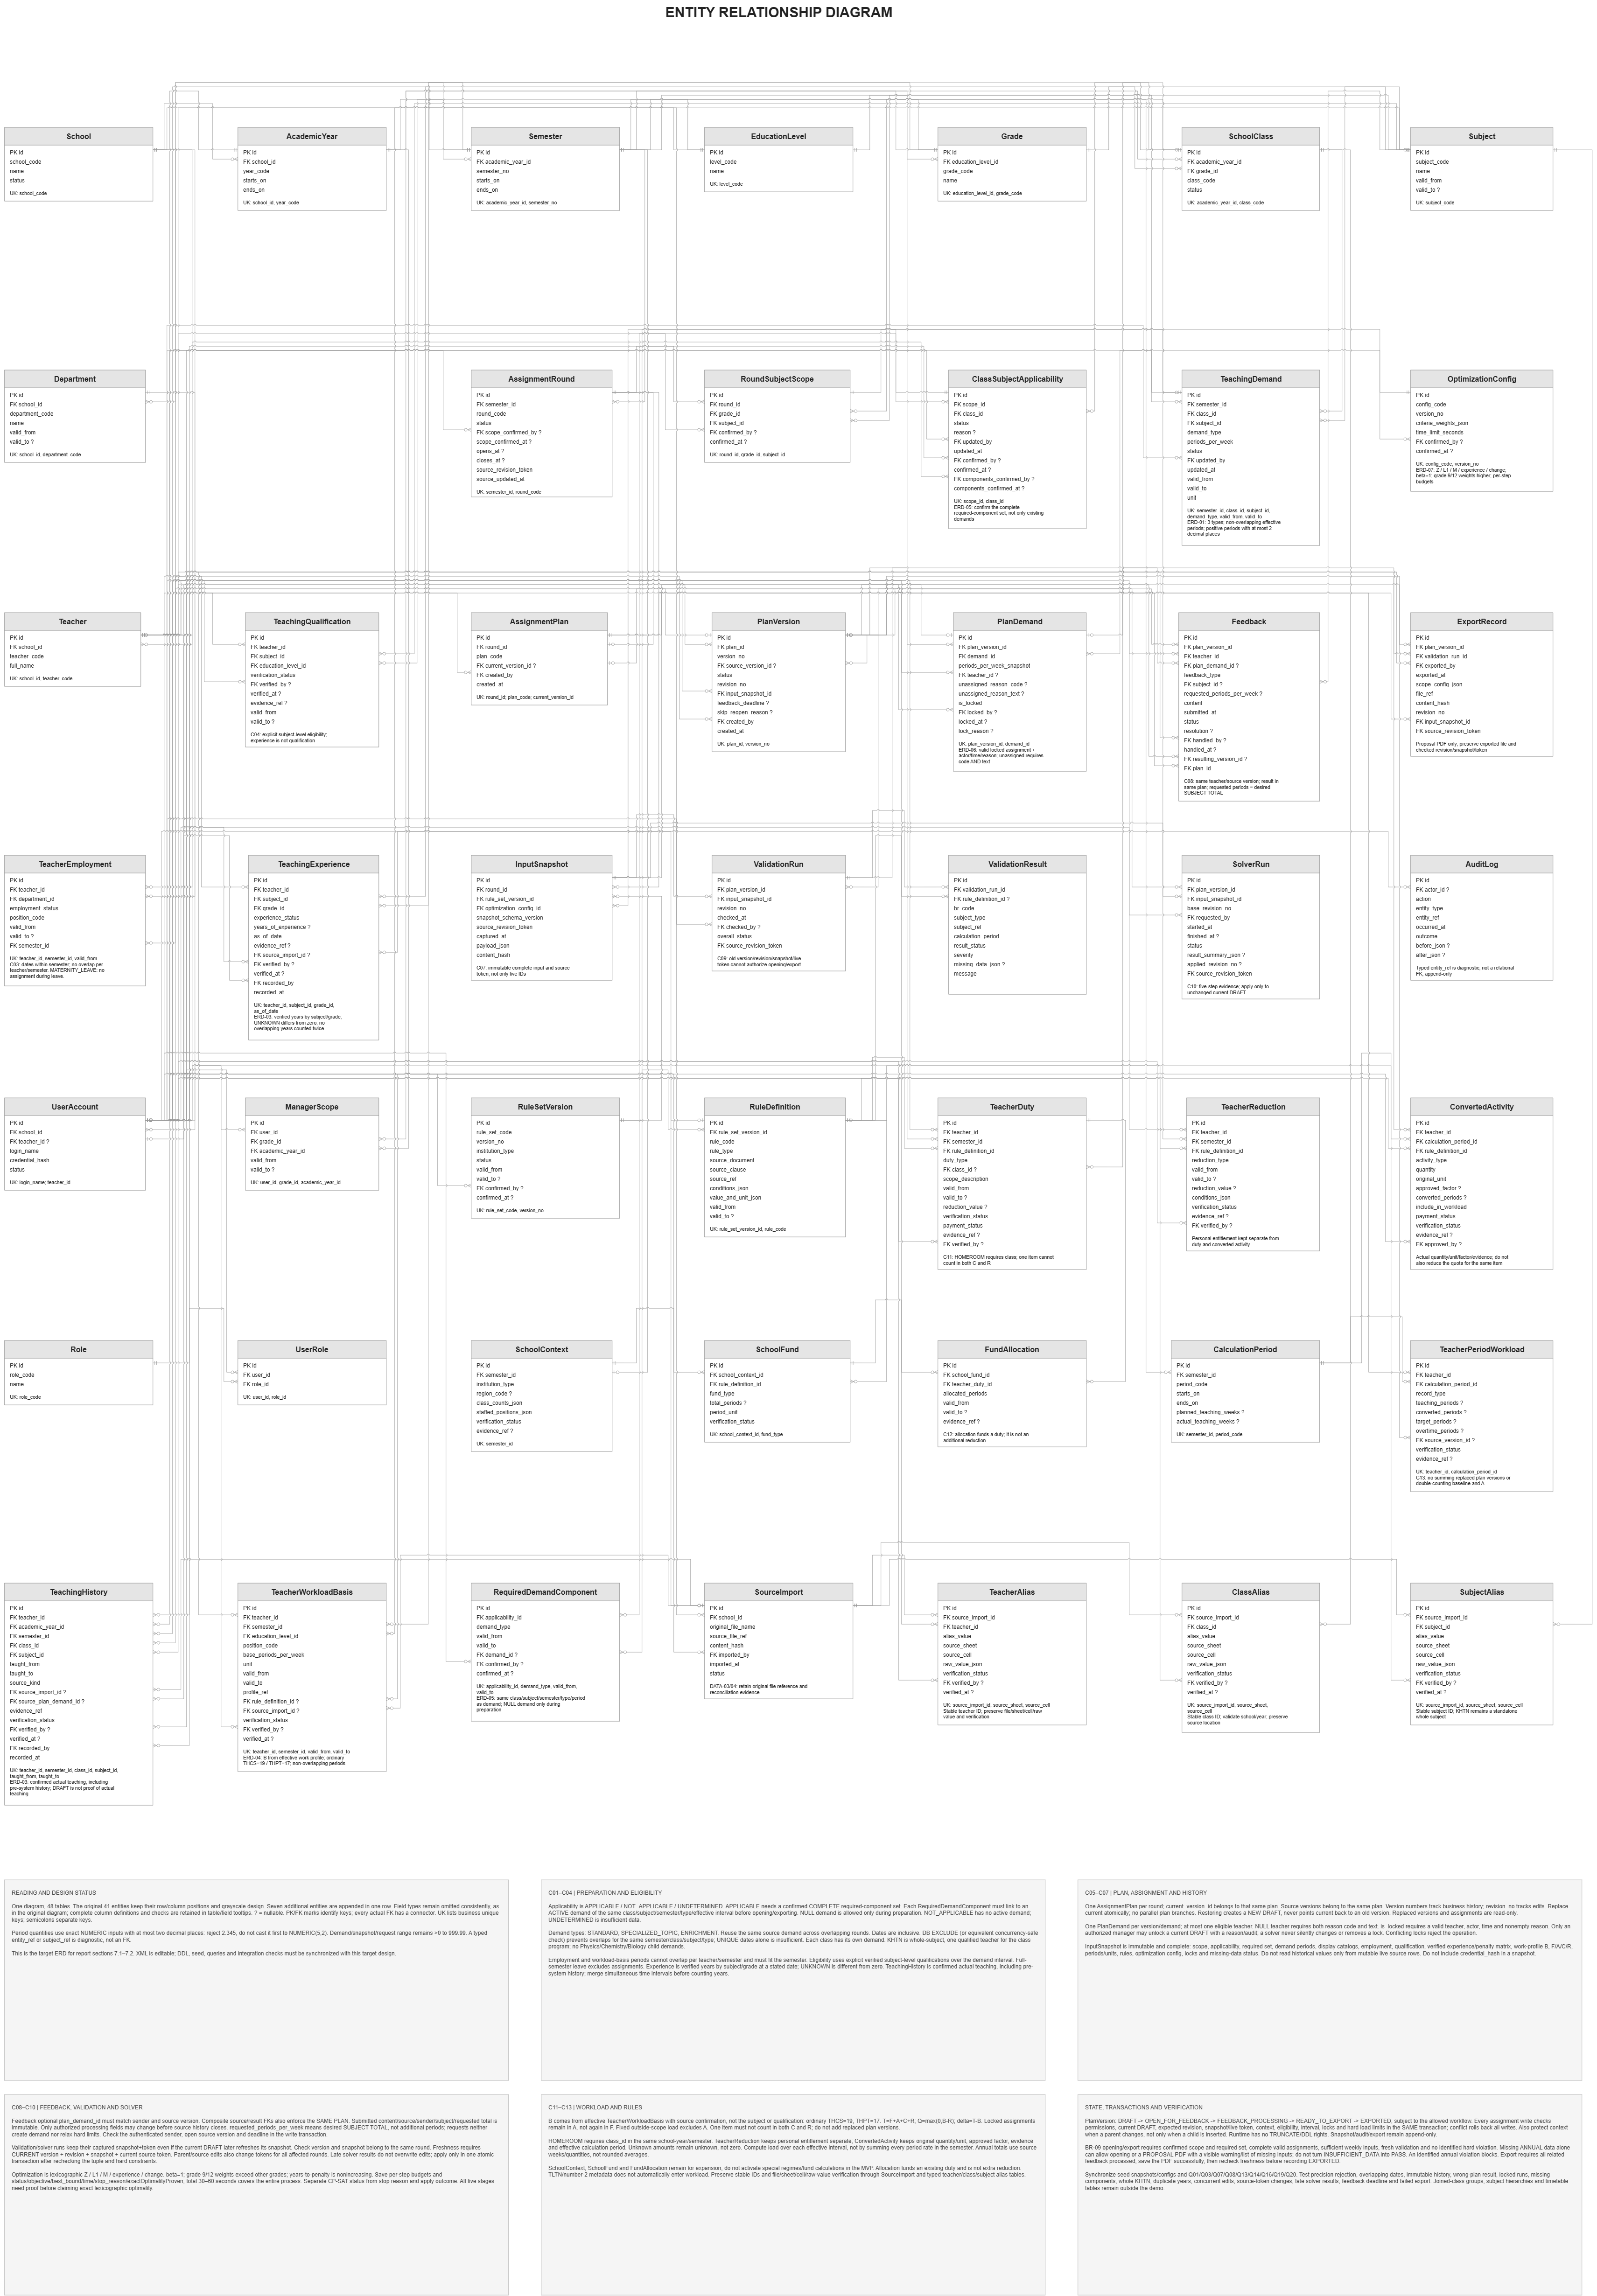
\includegraphics[width=0.98\linewidth,height=0.82\textheight,keepaspectratio]{diagrams/ERD_20261108.png}
\caption{ERD --- Quan hệ thực thể tổng quan, 48 bảng (08/11/2026)}\label{fig:ERD}
\end{figure}

\diagramtext{Trục AssignmentPlan--PlanVersion--PlanDemand lưu phương án, phiên bản và phân công. TeachingHistory lưu quá trình thực dạy; TeacherWorkloadBasis xác định định mức theo hồ sơ và hiệu lực; RequiredDemandComponent khai báo tập thành phần cần đáp ứng. SourceImport cùng TeacherAlias, ClassAlias và SubjectAlias giữ nguồn đối soát. InputSnapshot, ValidationRun/Result, SolverRun và ExportRecord gắn dữ liệu với phiên bản, revision và token nguồn. Token tham gia khóa ngoại ghép với định danh snapshot; việc so token với nguồn hiện tại giúp xác định dữ liệu còn hiệu lực.}

TeachingDemand lưu riêng STANDARD, SPECIALIZED\_TOPIC và ENRICHMENT theo lớp--môn--học kỳ--giai đoạn. Các khoảng ngày được tính cả hai đầu; ràng buộc EXCLUDE ngăn chồng hiệu lực của cùng khóa nghiệp vụ, đồng thời bảo vệ khoảng công tác và cơ sở định mức. Số tiết dùng NUMERIC không ép trước về hai chữ số; CHECK yêu cầu giá trị dương, không quá 999,99 và bằng giá trị cắt đến hai chữ số thập phân. Vì vậy, đầu vào 2,345 bị từ chối thay vì tự làm tròn.

TeachingExperience phân biệt HAS\_EXPERIENCE, NO\_EXPERIENCE và UNKNOWN, lưu số năm theo môn/khối tại as\_of\_date cùng nguồn xác nhận. Số năm bằng 0 ứng với chưa có kinh nghiệm; UNKNOWN để số năm NULL. TeachingHistory lưu khoảng thực dạy có chứng cứ; khi tổng hợp phải hợp các khoảng thời gian đồng thời trước khi tính số năm. TeacherWorkloadBasis cung cấp B theo cấp công tác và hiệu lực, tách khỏi môn dạy và năng lực chuyên môn.

RequiredDemandComponent khai báo tập bắt buộc độc lập với các nhu cầu đã có. Trong giai đoạn chuẩn bị, demand\_id có thể NULL để thể hiện còn thiếu nhu cầu; trước mở lấy ý kiến hoặc xuất tài liệu phải liên kết đúng lớp, môn, học kỳ, loại và giai đoạn. ClassSubjectApplicability xác nhận cả trạng thái áp dụng lẫn tính đầy đủ của tập thành phần; thay đổi tập này làm mất xác nhận cũ.

PlanDemand lưu is\_locked, người, thời điểm và lý do khóa; phân công chưa gán có cả mã và nội dung lý do. Các khóa ngoại ghép bảo đảm phiên bản hiện hành và phiên bản kết quả phản hồi thuộc đúng phương án. Trigger bảo vệ lịch sử, nội dung phản hồi, snapshot và nhật ký; thao tác sửa phân công làm tăng revision. Các kiểm tra quyền người dùng, giới hạn tải và áp dụng kết quả đồng thời tiếp tục được hoàn thiện ở tầng dịch vụ theo Mục~\ref{sec:future-work}.

\subsection{Bộ SQL và dữ liệu minh họa}
Bộ thiết kế đối chiếu trong lần cập nhật này là ba tệp \code{01_schema.sql}, \code{02_seed.sql}, \code{03_queries.sql} tại thư mục gốc \code{DACN/}, sử dụng theo thứ tự đó trên PostgreSQL 15 trở lên. Tệp schema tạo mới 48 bảng cùng khóa ngoại, ràng buộc, view và hàm; việc đưa vào database đã có dữ liệu cần migration riêng. SourceImport phục vụ truy vết nguồn và nhập dữ liệu đã chuẩn hóa, không bổ sung yêu cầu import Excel hàng loạt vào MVP.

Seed minh họa có 5 giáo viên, 6 lớp của năm hiện hành và 2 lớp lịch sử, 3 môn (Vật lý, Toán, KHTN), 10 nhu cầu theo giai đoạn, 14 thành phần bắt buộc của hai đợt và hai phiên bản phương án. Đợt chính có 10 thành phần đã gán trong phương án mẫu; đợt chuẩn bị cố ý còn trạng thái chưa xác định và liên kết thiếu. Hai bản ghi TeachingHistory của cùng giáo viên dạy đồng thời hai lớp minh họa việc không cộng trùng thời gian. Đây là dữ liệu tổng hợp để đối chiếu cấu trúc, chưa phải bản chuẩn hóa toàn bộ E3.

OptimizationConfig kiểm tra hợp đồng Z/L1/M/experience/change, $\beta=1$, trọng số khối 9/12 cao hơn khối khác và ngân sách từng bước. Cấu hình seed minh họa dùng trọng số 3 cho khối 9/12, 1 cho khối khác; điểm phạt lần lượt 6, 4, 2, 0 tại các ngưỡng 0, 1, 3, 5 năm. Tổng ngân sách 60 giây gồm 50 giây cho năm bước và 10 giây cho phần còn lại của quy trình. Các giá trị này là cấu hình demo, không phải ngưỡng nghiệp vụ bắt buộc. Giới hạn tổng tải 25 tiết/tuần trong seed cũng có nhãn minh họa, không dùng làm ngưỡng pháp lý mặc định.

Các hàm \code{tass_capture_snapshot} và \code{tass_snapshot_weekly_load} hỗ trợ chụp đầu vào và đọc tải tại một ngày hiệu lực. Theo seed, tổng A kỳ vọng của V2 là 27 tiết/tuần tại 15/10/2026 và 26,5 tại 15/11/2026; không cộng cả hai giai đoạn thành một tải tuần. Kiểm tra năm giữ INSUFFICIENT\_DATA khi thiếu HK2 và tổng năm. SolverRun mẫu có năm bước NOT\_RUN, kết quả NOT\_APPLIED; dữ liệu phương án mẫu không được trình bày thành kết quả solver đã chạy.

Tệp truy vấn có 32 nhóm Q01--Q32 để đối chiếu số lượng, bao phủ, tải theo hiệu lực, lịch sử, khóa, điểm kinh nghiệm, token và dữ liệu nguồn. Các kết quả nêu trên là giá trị kỳ vọng được mô tả trong seed/query; lần biên tập này chỉ đối chiếu mã SQL và nội dung ERD, chưa chạy bộ mới trên PostgreSQL. Mục~\ref{sec:future-work} nêu phần đồng bộ và kiểm chứng còn lại.


\section{Chuẩn hóa dữ liệu Excel}\label{sec:excel}
Nguồn E3 [31] là \code{TỔ VẬT LÝ - PCCM NH26-27.xlsx}, năm 2026--2027; dùng \code{Tổ VẬT LÝ NH 26-27} (Bảng Tổ) và \code{PCCM 2026 _ 2027} (Bảng Trường), ưu tiên Bảng Tổ sau ánh xạ ID. E1 [29] là dự kiến; E2 [30] và sheet năm cũ chỉ đối sánh/hồi quy, không trộn vào nhu cầu năm mới.

Ô trống trong nguồn nhu cầu E3 là không phát sinh, khác với teacher\_id NULL của nhu cầu áp dụng chưa gán trong DRAFT. Trạng thái nghỉ của giáo viên được xác định từ hồ sơ công tác và thời gian hiệu lực.

\begin{longtable}{|p{3.5cm}|p{10.4cm}|}
\hline
\textbf{Nguồn / ký hiệu} & \textbf{Quy tắc chuẩn hóa} \\\hline
\endfirsthead
\hline
\textbf{Nguồn / ký hiệu} & \textbf{Quy tắc chuẩn hóa} \\\hline
\endhead
G4/V4; D10--H10; G12/H12 & Các ô này thể hiện số tiết mỗi tuần của một lớp. Tổng số tiết được tính bằng số lớp nhân với số tiết mỗi lớp; ví dụ $4\times1.25=5$ và $3\times1.4=4.2$. \\\hline
\code{2+1*}; \code{tt}; \code{TH} & 2 thường + 1 chuyên đề/tuần; không nhân hệ số từ *. tt là ENRICHMENT, TH ở cột lớp là bí danh cần ánh xạ. \\\hline
E61/G61: 10A2 & G61=3 là tổng STANDARD=2 và SPECIALIZED\_TOPIC=1, cùng cô Đỗ Trúc. Tạo hai thành phần, không thêm nhu cầu tổng 3 hoặc suy loại chỉ từ nhãn CHUYÊN ĐỀ. \\\hline
E79/F79/G79: 12A1 & Cô Đỗ Trúc dạy 2 tiết thường của 12A1. Theo quy ước demo đã xác nhận, nhãn chuyên đề A1+A2 được tách thành hai nhu cầu của 12A1 và 12A2, mỗi lớp 1 tiết; cô Lơn dạy cả hai thì tải là 2 tiết/tuần. Giữ nguyên nhãn nguồn để đối soát; không biểu diễn một tiết dùng chung cho hai lớp. \\\hline
F3/U3; F63/F46/F28 & HK1 18/HK2 17 tuần. \code{0/2}: HK1 0, HK2 2 tiết; \code{2/0} ngược lại; / không là phép chia. \\\hline
B15/S15/AH15; S48/AG48 & Trần Thị Ngọc Liên hồ sơ THPT dùng B=17 dù môn KHTN. Nguyễn Thị Thanh Trúc ghi THCS/TLTN/số 2: dùng B=19 trong MVP, giữ nhãn/số nguồn, không suy giảm 17. \\\hline
B65/S65; C31/D37 & Thỉnh giảng ngoài cơ chế tải MVP; lọc ứng viên nhưng giữ nhu cầu. KHTN/Lý/CN không tự sinh quyền dạy. Quy mô theo bản chụp dữ liệu chuẩn hóa, không mặc định 10 giáo viên/40+ nhu cầu. \\\hline
F29 so E28/G28; E54/E72/E77 & Giữ hậu tố lớp như 9A1Đ và bí danh TH tới khi ánh xạ; tên rút gọn không là khóa, không ghép người theo tên Trúc. Sai khác hai bảng lưu cả giá trị nguồn và căn cứ chọn. \\\hline
HSG; U23/W23/AC23 & X HSG là nhiệm vụ/thù lao riêng, không tự quy thành tiết dạy tuần hoặc hệ số giảm. Chi tiết HK2 để trống không đủ căn cứ kết luận giáo viên nghỉ toàn kỳ. \\\hline
\end{longtable}

Quy trình chuẩn hóa gồm năm bước: (1) lưu vị trí tệp, bảng tính và ô dữ liệu, giá trị gốc, mã SHA-256 và ngày trích xuất; (2) ánh xạ ID và bí danh, đồng thời đối soát hai bảng; (3) xác nhận phạm vi, thành phần, đơn vị và hiệu lực, phân biệt dòng tổng với chi tiết; (4) tính toán bằng số thập phân chính xác, không cộng số lớp của các môn thành số lớp duy nhất; (5) phân loại B/R/F/A/C và xác nhận chuyên môn trước khi tạo bản chụp dữ liệu. Hệ thống dừng bước kiểm tra đầu vào nếu thiếu dữ liệu bắt buộc, thay vì quy đổi giá trị chưa biết thành 0.

Trình tự phối hợp khi chuẩn bị dữ liệu được thể hiện bằng sơ đồ hoạt động phân làn tại Hình~\ref{fig:DG-03}. Sơ đồ nối việc quản trị danh mục và học kỳ với bước xác nhận chuyên môn, phạm vi áp dụng và nhu cầu của Academic Manager trước khi lập phương án.

\begin{figure}[H]
\centering
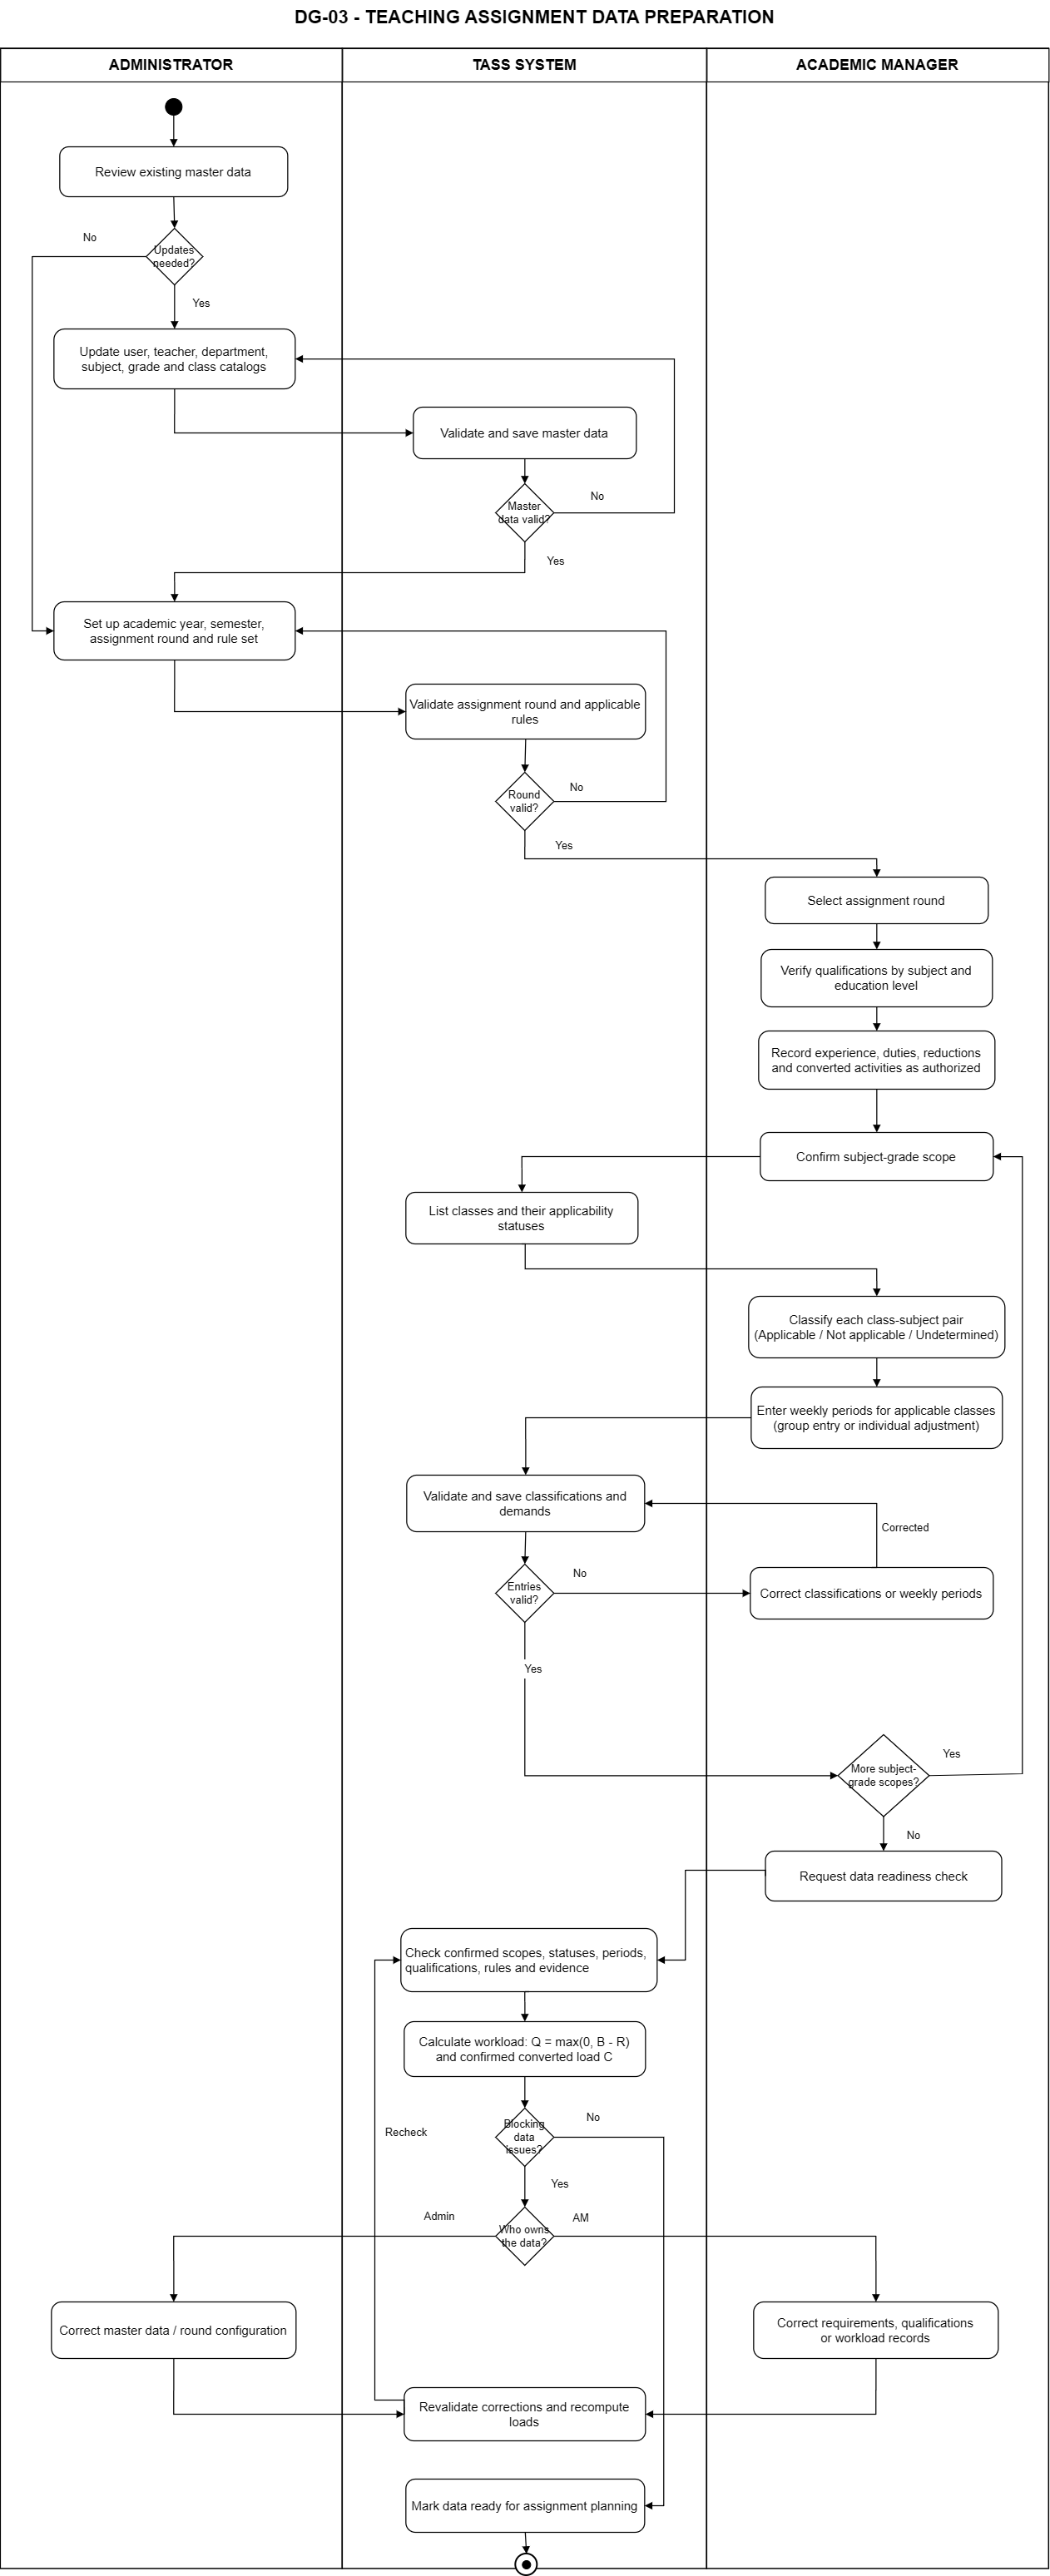
\includegraphics[width=0.98\linewidth,height=0.70\textheight,keepaspectratio]{diagrams/DG-03.png}
\caption{DG-03 --- Hoạt động chuẩn bị dữ liệu}\label{fig:DG-03}
\end{figure}

\diagramtext{Luồng kiểm tra được lặp theo từng phạm vi môn--khối; dữ liệu sai quay lại người có trách nhiệm để sửa và kiểm tra lại. Trước khi báo sẵn sàng, hệ thống phải xét đủ thành phần bắt buộc và đầu vào cho các ràng buộc đang áp dụng, không chỉ các dòng nhu cầu đã nhập. Trạng thái thiếu riêng dữ liệu năm được xử lý theo BR-09.}


\section{Kiến trúc và triển khai}\label{sec:deployment}

Hình~\ref{fig:DG-09} mô tả cách bố trí TASS trên ba thành phần triển khai: thiết bị dùng trình duyệt, máy chủ ứng dụng và cơ sở dữ liệu. Các đường kết nối thể hiện trao đổi yêu cầu/kết quả với người dùng và truy cập dữ liệu bền vững của ứng dụng.

\begin{figure}[H]
\centering
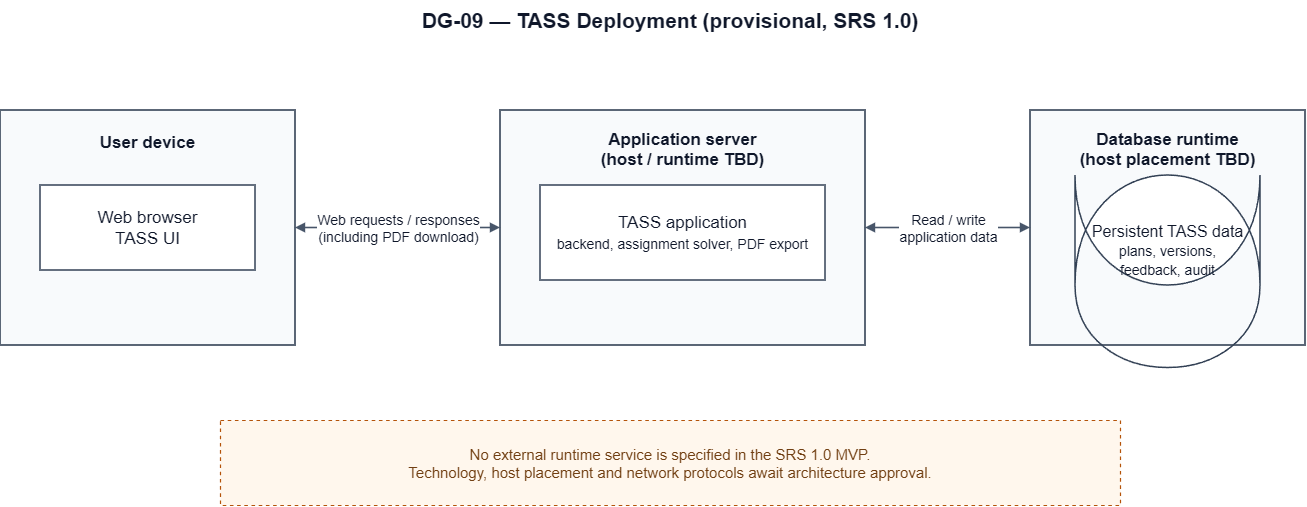
\includegraphics[width=0.98\linewidth,height=0.38\textheight,keepaspectratio]{diagrams/DG-09.png}
\caption{DG-09 --- Triển khai TASS}\label{fig:DG-09}
\end{figure}

\diagramtext{Máy chủ thực hiện nghiệp vụ phân công, gọi thư viện OR-Tools và sinh PDF; trình duyệt nhận kết quả và tải tài liệu. Cơ sở dữ liệu giữ phương án, phiên bản, phản hồi và nhật ký. Sơ đồ thể hiện kiến trúc định hướng của MVP; công nghệ máy chủ và vị trí triển khai sẽ được xác định trong thiết kế vận hành. Nhãn provisional/SRS 1.0 trong ảnh được giữ theo bản vẽ nguồn. OR-Tools được sử dụng như thư viện trên máy chủ ứng dụng, không phải một dịch vụ Google bên ngoài.}


\chapter{THIẾT KẾ THUẬT TOÁN PHÂN CÔNG}\label{chap:math-model}
Chương này chuyển các quy tắc phân công thành mô hình tối ưu rời rạc. Sau khi phân tích lựa chọn bộ giải, các phần tiếp theo xác định đầu vào, biến quyết định, ràng buộc, thứ tự mục tiêu và điều kiện ghi nhận kết quả vào phương án hiện hành.


\section{Lựa chọn CP-SAT}\label{sec:algorithm-choice}
Dạng tổng quát của bài toán phân công thuộc lớp NP-khó; bài toán phân hoạch có thể biểu diễn như một trường hợp riêng. Với m giáo viên và n nhu cầu, không gian vét cạn có tới $(m+1)^n$ khả năng, kể cả lựa chọn chưa phân công; kích thước này không trực tiếp dự báo thời gian thực thi. CP-SAT kết hợp lan truyền ràng buộc, học mệnh đề và quy hoạch tuyến tính (LP) [25]. Bộ giải phù hợp với các quyết định Boolean hoặc số nguyên, đồng thời cung cấp nghiệm khả thi tốt nhất đã tìm được (incumbent) và cận của giá trị mục tiêu (bound) khi dừng sớm [22, 23].

\begin{longtable}{|p{3.2cm}|p{10.7cm}|}
\hline
\textbf{Phương pháp} & \textbf{Đánh giá trong TASS} \\\hline
\endfirsthead
\hline
\textbf{Phương pháp} & \textbf{Đánh giá trong TASS} \\\hline
\endhead
Hungarian / Min-Cost Flow & Các phương pháp này hiệu quả nếu bài toán có thể quy về ghép cặp hoặc luồng trên mạng. Để áp dụng cho TASS, cần chứng minh tính tương đương khi nhu cầu là nguyên khối và có nhiều giới hạn tải cùng mục tiêu công bằng. Thuật toán luồng có thể nhanh hơn nếu cấu trúc phù hợp [24]. \\\hline
MILP & Phương pháp quy hoạch tuyến tính nguyên hỗn hợp có thể biểu diễn các quyết định phân công, giới hạn tải và mục tiêu được tuyến tính hóa. Đây là lựa chọn đối chứng chính xác, cần được đánh giá với một bộ giải cụ thể. \\\hline
Greedy & Thuật toán tham lam đơn giản và có thời gian xử lý ngắn, phù hợp làm đối chứng. Chất lượng phương án phụ thuộc thứ tự phân công và không được bảo đảm tối ưu. \\\hline
GA / tìm kiếm cục bộ & GA đã có trong bộ thuật toán đối chứng; chất lượng phụ thuộc cách mã hóa, sửa phương án và tham số tìm kiếm. Thuật toán không cung cấp bằng chứng tối ưu trong phạm vi thực nghiệm này. Local Search, SA và Tabu là các hướng mở rộng, chưa thuộc PoC. \\\hline
CP-SAT & Bộ giải được chọn vì hỗ trợ biến Boolean, số nguyên, ràng buộc khóa, giới hạn tải và quan hệ cực đại. Kết quả có thể kèm cận và bằng chứng tối ưu. Mô hình cần hệ số tỷ lệ chính xác, miền hữu hạn và thư viện native phù hợp hệ điều hành; giới hạn thời gian có thể kết thúc trước khi chứng minh được tính tối ưu. \\\hline
\end{longtable}

OR-Tools được phát hành theo giấy phép Apache-2.0 [26]; việc đóng gói phải quản lý phiên bản và thư viện thực thi phù hợp với hệ điều hành. CP-SAT được lựa chọn vì khả năng biểu diễn ràng buộc và kiểm chứng chất lượng nghiệm. Lựa chọn này không hàm ý bộ giải luôn nhanh hơn hoặc tạo nghiệm tốt hơn trên mọi dữ liệu. Tầng ứng dụng và bộ kiểm tra vẫn chịu trách nhiệm xác thực chuyên môn, phân quyền và dữ liệu đầu vào.

\section{Tập hợp, tham số và chuẩn hóa}\label{sec:solver-input}
Một lượt giải thuộc một trường, một học kỳ, một đợt và một DRAFT hiện hành.
$G$ là tập giáo viên được xét; $D$ là tập thành phần nhu cầu áp dụng, đang
hiệu lực trong phạm vi đợt. Mỗi $j\in D$ có ID bất biến, một lớp, một môn, kỳ, loại và khoảng hiệu lực. KHTN được biểu diễn bằng nhu cầu toàn môn của lớp, không tách Lý/Hóa/Sinh.
$K$ là tập các cặp lớp--môn trong học kỳ; $D_k$ là các thành phần của cặp $k$.
$E\subseteq G\times D$ là các cặp đủ điều kiện đã xác nhận; $H_i$ là tập
hoạt động quy đổi được chọn của giáo viên $i$.

\begin{longtable}{|p{2.3cm}|p{11.6cm}|}\hline
Ký hiệu & Ý nghĩa và yêu cầu nguồn \\\hline\endfirsthead
\hline Ký hiệu & Ý nghĩa và yêu cầu nguồn \\\hline\endhead
$B_i,R_i,Q_i$ & Định mức cơ sở thông thường THCS=19/THPT=17 theo hồ sơ/chức danh, giảm trừ hợp lệ và mục tiêu đối chiếu phụ $Q_i=\max(0,B_i-R_i)$ theo bộ quy tắc đã xác nhận. \\\hline
$F_i$ & Tải giảng dạy cố định ngoài $D$, từ một nguồn được chọn; không bao gồm gán đã nằm trong $D$ và không cộng lịch sử thay thế. \\\hline
$C_i$ & Tải quy đổi hợp lệ, cùng kỳ và đơn vị; không tự lấy hệ số trần, không cộng trùng nhiệm vụ đã giảm trừ. \\\hline
$h_j$ & Số tiết của thành phần $j$; dương, đầu vào có tối đa hai chữ số thập phân, có đơn vị và kỳ tính. \\\hline
$e_{ij}$ & 1 nếu cặp $i,j$ đáp ứng công tác, phạm vi, chuyên môn môn--cấp và hiệu lực; kinh nghiệm không thay điều kiện này. \\\hline
$p_{ij}$ & Điểm phạt kinh nghiệm nguyên không âm của cặp giáo viên--nhu cầu hợp lệ, tính theo kinh nghiệm giảng dạy môn/khối đã ghi nhận và quy tắc có phiên bản; phù hợp hơn thì điểm thấp hơn. Không phải hệ số quy đổi pháp lý. \\\hline
$w_j,\beta$ & Trọng số kinh nghiệm nguyên dương của nhu cầu và hệ số chung $\beta=1$. Dùng $w_j=w_{\mathrm{cuoi}}$ cho khối 9/12, $w_j=w_{\mathrm{khac}}$ cho các khối còn lại, với $w_{\mathrm{cuoi}}>w_{\mathrm{khac}}>0$; giá trị cụ thể lưu trong OptimizationConfig. \\\hline
$U_{ir},a_{irj}$ & Giới hạn của phép kiểm tra cứng $r$ cho giáo viên $i$ và hệ số tải được phép tính cho gán $i,j$ trong chính phép kiểm tra đó. \\\hline
\end{longtable}
Giáo viên nghỉ toàn kỳ không được tính vào mục tiêu cân bằng tải; trường hợp nghỉ một phần kỳ được xét theo từng giai đoạn hiệu lực. Các chế độ đặc thù ngoài MVP được loại khỏi tập ứng viên, trong khi nhu cầu chương trình vẫn được giữ. Trước khi dựng mô hình, hệ thống kiểm tra tập thành phần bắt buộc, trạng thái áp dụng, số tiết, công tác, năng lực chuyên môn và tải theo các yêu cầu DATA và BR. Nếu thiếu dữ liệu để thiết lập điều kiện đang xét, quá trình giải phải dừng ở bước kiểm tra đầu vào. Trường hợp chỉ thiếu dữ liệu năm được xử lý theo BR-09.

Số tiết nhu cầu nhập vào có tối đa hai chữ số thập phân; hệ thống kiểm tra trước khi ghi DB và từ chối giá trị vượt độ chính xác, không tự cắt hoặc làm tròn. Số tiết quy đổi được tính theo $C_i=\sum_{a\in H_i}q_{ia}k_{ia}$ bằng số thập phân chính xác hoặc số hữu tỷ, cùng kỳ tính và đơn vị, không tính lại các khoản thuộc R. Hệ số tỷ lệ S được chọn để biểu diễn chính xác mọi hệ số tải của mô hình bằng số nguyên. Khi mọi hệ số tải có tối đa hai chữ số thập phân, dùng S=100, chẳng hạn $1.25\mapsto125$; nếu phép quy đổi sinh hệ số có độ chính xác cao hơn, chọn S phù hợp để giữ nguyên giá trị tính được. Việc chuẩn hóa kết quả tính không mở rộng độ chính xác được phép của đầu vào nhu cầu. Kiểm tra miền giá trị, nguy cơ tràn số và lưu giá trị gốc, đơn vị, S trong snapshot theo DATA-09/13/18. Ký hiệu tải từ đây biểu diễn số nguyên chuẩn hóa; kết quả hiển thị được chuyển về đơn vị nghiệp vụ.

\section{Biến và biểu thức tải}\label{sec:variables}
\paragraph{Biến phân công.}
$x_{ij}\in\{0,1\}$ với $(i,j)\in E$: bằng 1 khi gán giáo viên $i$ cho thành
phần $j$. Chỉ tạo biến cho tập $E$ để giảm kích thước mô hình. Trong công
thức, quy ước $x_{ij}=0$ nếu $(i,j)\notin E$.
\paragraph{Biến chưa phân công.}
$y_j\in\{0,1\}$: bằng 1 khi thành phần $j$ chưa có giáo viên.
\paragraph{Biến độ lệch.}
$under_i,over_i$ là số nguyên không âm có miền hữu hạn, tính trên giáo viên có định mức áp dụng và đủ dữ liệu. Không tạo biến liên kết để ép cùng giáo viên giữa các thành phần trong MVP. Gán thủ công đã chốt được giữ bằng khóa HC-04; gán khóa vẫn thuộc A, không cộng lại vào F.


\[A_i=\sum_{j\in D}h_jx_{ij}.\]
Mỗi nhu cầu của một lớp đóng góp một số hạng vào tải giáo viên. Ví dụ hai nhu cầu chuyên đề của 12A1 và 12A2, mỗi nhu cầu 1 tiết và cùng được gán cho một giáo viên, đóng góp tổng 2 tiết. Các đại lượng W, T và Q được xác định theo (\ref{eq:workload}); độ lệch chính được tính giữa T và B:
\[
under_i=\max(0,B_i-T_i),\qquad over_i=\max(0,T_i-B_i).
\]
Mô hình sử dụng AddMaxEquality để xác định chính xác cả hai biến ở mọi bước. Đẳng thức $T_i-B_i=over_i-under_i$ chưa đủ, vì hai biến vẫn có thể cùng dương khi độ lệch chưa được tối ưu. Với $0\le T_i\le T_i^{\max}$, các miền an toàn là $0\le under_i\le B_i$ và $0\le over_i\le\max(0,T_i^{\max}-B_i)$; mọi cận đều được tính từ dữ liệu hữu hạn. Biểu diễn W/Q chỉ tương đương khi $R_i\le B_i$; tính tương đương không được mặc định khi Q bị chặn tại 0.



\section{Ràng buộc cứng và tiền điều kiện}\label{sec:hard-constraints}
\paragraph{HC-01 --- Một kết quả mỗi thành phần và liên kết giáo viên theo chính sách}
\[
\sum_{i\in G}x_{ij}+y_j=1\quad(j\in D).
\]
MVP không áp ràng buộc cùng giáo viên cho toàn bộ cặp lớp--môn. STANDARD và SPECIALIZED\_TOPIC có thể cùng hoặc khác giáo viên, không phát sinh điểm phạt chỉ vì khác giáo viên. Mỗi thành phần vẫn có tối đa một giáo viên; gán khóa theo HC-04 được giữ.
KHTN dùng một nhu cầu chương trình toàn môn cho mỗi lớp/giai đoạn, nên biến phân công chọn một giáo viên đủ chuyên môn KHTN; không tạo các nhu cầu con Lý/Hóa/Sinh hoặc cộng thêm tải phân môn vào tải toàn môn. DRAFT có thể thiếu gán; mở lấy ý kiến hoặc xuất tài liệu theo BR-09.

\paragraph{HC-02 --- Đúng chuyên môn, công tác và phạm vi}
$x_{ij}\le e_{ij}$. Chỉ dùng năng lực môn--cấp đã xác nhận và hiệu lực đáp
ứng nhu cầu, cùng TeacherEmployment đúng học kỳ. Môn gần giống, tổ chuyên
môn hoặc kinh nghiệm không tự sinh quyền dạy. Chuyên môn nhóm môn cần ánh
xạ cụ thể đã xác nhận; không coi một chứng chỉ riêng là đủ cho mọi môn tích hợp.
\paragraph{HC-03 --- Các giới hạn tải đã xác nhận}
Với mỗi phép kiểm tra cứng $r$ đủ dữ liệu và được áp dụng:
\[
L_{ir}=F_{ir}+C_{ir}+\sum_j a_{irj}x_{ij}\le U_{ir}.
\]
$F_{ir},C_{ir},a_{irj}$ là các thành phần được phép tính trong chính phép
kiểm tra đó. Trong trường hợp minh họa đơn giản, $a_{irj}=h_j$ và $L_{ir}=W_i$ nếu đã
xác nhận đúng định nghĩa. Không tự dùng $1.5Q_i$ làm trần. Vi phạm cứng đã
xác định không đổi thành phạt mềm; thiếu dữ liệu không tự báo PASS.
\paragraph{HC-04 --- Khóa gán cứng}
$lock_{ij}=1\Rightarrow x_{ij}=1$ và $y_j=0$. Khóa chỉ định một giáo viên cho một nhu cầu; kiểm tra tồn tại, chuyên môn, hiệu lực và tải trước giải. Gán thủ công/đã chốt được giữ khóa khi chạy lại. Academic Manager có quyền mở khóa trên DRAFT và phải lưu dấu vết. Hai khóa xung đột hoặc khóa không còn hợp lệ trả LOCK\_CONFLICT, giữ DRAFT, không âm thầm bỏ khóa hay đổi giáo viên. Nhu cầu khóa vẫn nằm trong A, không cộng lại vào F.

\paragraph{HC-05 --- Gán cấm: ngoài phạm vi MVP}
Chưa kích hoạt như chức năng quản lý riêng trong PoC lõi. Nếu được duyệt,
$ban_{ij}=1\Rightarrow x_{ij}=0$; không tự thêm ma trận cấm ngoài căn cứ
điều kiện chuyên môn đã có.
\paragraph{HC-06 --- Tiền kiểm dữ liệu kiêm nhiệm và quy đổi}
Hệ thống kiểm tra loại khoản, giáo viên, kỳ tính, hiệu lực, đơn vị và giá trị của đầu vào minh họa; nhiệm vụ GVCN phải tham chiếu lớp. Mỗi khoản chỉ được tính một lần vào C hoặc R. Các mức kiêm nhiệm và quy đổi được sử dụng theo BR-16; hệ thống không suy thêm khoản giảm từ ghi chú TLTN hoặc số 2.

\paragraph{HC-07 --- Giới hạn phạm vi, không phải phép kiểm tra lịch}
Mô hình hiện tại không khai báo biến thời gian hoặc phòng học, vì vậy hệ thống không kiểm tra xung đột lịch, trùng phòng hoặc thời gian di chuyển. Chức năng xếp thời khóa biểu thuộc phạm vi mở rộng độc lập với mô hình phân công hiện hành.



\section{Mục tiêu và tối ưu năm bước}\label{sec:objectives}
Thứ tự nghiệp vụ là độ phủ, cân bằng tải, kinh nghiệm giảng dạy và hạn chế xáo trộn. Do cân bằng tải gồm hai mục tiêu liên tiếp là tổng lệch L1 và độ lệch lớn nhất, quy trình thực hiện năm bước tối ưu. Mọi bước đều tuân thủ các ràng buộc cứng và giữ nguyên các phân công đã khóa.
\paragraph{SC-01 --- Giảm phần chưa phân công}
\[
Z=\sum_{j\in D}c_jy_j.
\]
Mô hình sử dụng $c_j=1$ theo chế độ COMPONENTS, tức mỗi thành phần nhu cầu của từng lớp có cùng trọng số. Hai nhu cầu của 12A1 và 12A2 được đếm riêng. Việc tối thiểu hóa số thành phần thiếu không bảo đảm mọi lớp đều có giáo viên hoặc số cặp lớp--môn hoàn chỉnh đạt tối đa.

Báo cáo đồng thời số thành phần, số tiết thiếu và số cặp lớp--môn chưa đủ.
\paragraph{SC-02 --- Tổng lệch và độ lệch lớn nhất}
\[
d_i=under_i+over_i=|T_i-B_i|,\quad E_{load}=\sum_{i\in G^*}d_i,\quad M=\max_{i\in G^*}d_i.
\]
$G^*$ gồm giáo viên có mục tiêu áp dụng và đủ dữ liệu trong tổ đang xét; loại người nghỉ toàn kỳ; ca thỉnh giảng nằm ngoài phạm vi G của MVP. Nếu $G^*$ rỗng, Eload=M=0. Dùng AddMaxEquality để mô hình M trên miền hữu hạn. Tối thiểu L1 trước, sau đó cố định L1 và tối thiểu M. Ví dụ B=(10,10): tổng tải (10,0) và (5,5) cùng L1=10 nhưng M=10 và 5.

\paragraph{SC-03 --- Ưu tiên kinh nghiệm, đặc biệt ở lớp cuối cấp}
Sau khi cố định độ phủ và hai mục tiêu cân bằng tải, hệ thống ưu tiên kinh nghiệm giảng dạy phù hợp với môn/khối. Điểm phạt kinh nghiệm của phương án là:
\[
E_{exp}=\sum_{(i,j)\in E}w_jp_{ij}x_{ij}.
\]
Nhu cầu thuộc khối 9 và khối 12 dùng trọng số $w_{\mathrm{cuoi}}$, cao hơn $w_{\mathrm{khac}}$ của các khối còn lại. Đây là mức ưu tiên cao hơn trong tổng điểm kinh nghiệm, không phải một tầng tối ưu riêng cho lớp cuối cấp. $p_{ij}$ được tính từ số năm kinh nghiệm theo đúng môn/khối, mốc tính và nguồn xác nhận trong hồ sơ; số năm tăng thì điểm phạt không tăng theo quy tắc đã cấu hình. Phân biệt chưa có kinh nghiệm với chưa đủ dữ liệu, không cộng trùng số năm khi dạy nhiều lớp cùng lúc. Quy tắc quy đổi số năm thành điểm và hai trọng số được lưu theo phiên bản cùng snapshot; thâm niên chung không tự thay thế kinh nghiệm phù hợp hoặc chuyên môn.

Bước này tối thiểu hóa $E_{exp}$ độc lập với các mục tiêu khác, tương ứng $\beta=1$. Nhân toàn bộ $E_{exp}$ với một hệ số dương khác không làm đổi thứ tự phương án; mức ưu tiên của lớp cuối cấp được thể hiện bằng $w_j$. Không cộng điểm kinh nghiệm vào một tổng trọng số chung với độ phủ hoặc tải. Vì độ phủ và tải đã được cố định, hệ thống không bỏ trống nhu cầu hoặc làm xấu cân bằng tải để cải thiện kinh nghiệm; chuyên môn, giới hạn tải và khóa vẫn là điều kiện cứng.

Ví dụ minh họa, hai nhu cầu Toán khối 8 và khối 9 có cùng số tiết; hai giáo viên A và B đều đủ chuyên môn. Giả sử A có điểm phạt 0, B có điểm phạt 5 đối với cả hai nhu cầu, và hai cách đổi chéo giáo viên có cùng Z, L1 và M. Với trọng số minh họa $w_{\mathrm{cuoi}}=3$, $w_{\mathrm{khac}}=1$, giao A cho lớp 9 và B cho lớp 8 có điểm $3\times0+1\times5=5$; giao ngược lại có điểm $3\times5+1\times0=15$. Phương án thứ nhất được ưu tiên dù có thể cần đổi phân công tự động chưa khóa. Các số 0, 5 và tỷ lệ 3:1 chỉ minh họa cách tính, không ấn định tham số vận hành.

\paragraph{SC-04 --- Hạn chế thay đổi khi chạy lại}
Gọi $D^0$ là nhu cầu cùng định danh ở cả bản chụp dữ liệu trước và hiện tại.
Nếu trước đây $j$ gán cho $i_0$, đặt $d_j=1-x_{i_0j}$; nếu trước đây chưa
gán, đặt $d_j=1-y_j$. $E_{chg}=\sum_{j\in D^0}d_j$. Đổi giáo viên đếm một
lần; nhu cầu thêm/xóa báo riêng. Giữ mềm không tương đương khóa cứng; chính
sách giữ/thay gán phải hiển thị trước khi chạy và được ghi trong cấu hình lượt chạy. Phương án làm mốc thuộc cùng đợt phân công và học kỳ; tiêu chí này không mặc định so sánh giữa hai học kỳ. Nếu không có phương án làm mốc, $E_{chg}=0$. Chỉ ưu tiên giữ phân công cũ sau khi đã cố định điểm kinh nghiệm; phân công tự động chưa khóa có thể được đổi để cải thiện các mục tiêu đứng trước.


Tối ưu theo thứ tự từ điển:
\[
\min_{lex}\ (Z,E_{load},M,E_{exp},E_{chg}).
\]
\begin{enumerate}
\item Giải tối thiểu Z; lưu nghiệm khả thi tốt nhất đã tìm được đã được bộ kiểm tra kiểm tra và giá trị $\widehat Z$.
\item Thêm $Z=\widehat Z$, giải tối thiểu Eload; lưu $\widehat E$.
\item Thêm $E_{load}=\widehat E$, giải tối thiểu M; lưu $\widehat M$.
\item Thêm $M=\widehat M$, giải tối thiểu $E_{exp}$; lưu $\widehat E_{exp}$.
\item Thêm $E_{exp}=\widehat E_{exp}$, giải tối thiểu $E_{chg}$.
\end{enumerate}
Mỗi bước duy trì toàn bộ các đẳng thức đã thiết lập ở những bước trước. Vì các mục tiêu được giải lần lượt thay vì cộng vào cùng một tổng trọng số, $E_{exp}$ và $E_{chg}$ không cần nhân với S để đồng nhất đơn vị với các mục tiêu tải.

\paragraph{Trạng thái, chứng minh và bảo toàn phương án.}
Mỗi bước ghi lại tên mục tiêu, trạng thái giải (status), giá trị mục tiêu (objective), cận tốt nhất (best bound), thời gian, nguyên nhân dừng và cờ \code{exactOptimalityProven}. Việc xác nhận tối ưu chính xác yêu cầu ngưỡng dừng theo độ lệch tối ưu (gap tolerance) bằng 0 và đối chiếu với cận. Chỉ khi cả năm bước đều có bằng chứng tối ưu, hệ thống mới xác nhận nghiệm tối ưu theo thứ tự từ điển.

Nếu một bước chỉ đạt FEASIBLE, hệ thống có thể cố định giá trị của nghiệm khả thi tốt nhất đã tìm được để cải thiện mục tiêu tiếp theo trong thời gian còn lại. Kết quả sau đó chỉ tối ưu có điều kiện trên các giá trị đã cố định; chẳng hạn, trạng thái OPTIMAL ở bước 5 không chứng minh Z tối ưu nếu bước 1 chưa có bằng chứng. Nếu bước đầu trả UNKNOWN hoặc INFEASIBLE mà không có nghiệm khả thi, hệ thống dừng và giữ nguyên DRAFT. Nếu bước sau không tìm được nghiệm mới, hệ thống sử dụng nghiệm đã kiểm tra từ bước trước. Kết quả INFEASIBLE ở bước sau, dù đã có nghiệm thỏa các đẳng thức cố định, phải được xem xét như một lỗi mô hình hoặc dữ liệu.

\paragraph{Giới hạn thời gian thực thi.}
Tổng thời gian xử lý được cấu hình trong khoảng 30--60 giây. Mục tiêu là toàn bộ quy trình không vượt quá 60 giây, bao gồm thời gian chờ, tạo bản chụp dữ liệu, kiểm tra đầu vào, thực hiện năm bước tối ưu, kiểm tra nghiệm và ghi nhận kết quả. OptimizationConfig lưu phần thời gian dành cho từng bước; giới hạn 60 giây không được cấp riêng cho mỗi bước. Khi hết thời gian còn lại, bộ giải dừng và bảo toàn nghiệm khả thi đã được kiểm tra. Gợi ý nghiệm ban đầu (solution hint) chỉ định hướng tìm kiếm, không thay thế khóa phân công hoặc bằng chứng tối ưu.



\section{Thực thi và áp dụng kết quả}\label{sec:solver-integration}
\begin{enumerate}
\item Kiểm tra quyền, DRAFT hiện hành, revision và cấu hình; lấy dữ liệu nhất quán.
\item Tạo InputSnapshot bất biến; kiểm tra trạng thái áp dụng, tập thành phần,
công tác học kỳ, chuyên môn, kinh nghiệm và điểm phạt theo cấu hình, đơn vị, tải và dữ liệu bắt buộc.
\item Tính/chuẩn hóa tham số, dựng biến thưa và ràng buộc; kiểm tra tính hợp lệ mô hình.
\item Khởi tạo bản ghi \code{SolverRun} và thực thi năm bước Z/L1/M/experience/change trong tổng ngân sách thời gian đã ấn định.
\item Giải mã nghiệm khả thi tốt nhất đã tìm được, sau đó kiểm tra độc lập dựa trên bản chụp dữ liệu.
\item Sinh số liệu và chẩn đoán có căn cứ; ghi rõ phần kiểm tra năm chưa đủ.
\item Chỉ ghi nhận kết quả trong một giao dịch nguyên tử nếu phương án, phiên bản DRAFT, số lần cập nhật và mã kiểm soát dữ liệu đầu vào vẫn trùng khớp. Giao dịch lưu PlanDemand, lý do chưa phân công, tải liên quan, thông tin áp dụng và số lần cập nhật mới.
\item Nếu dữ liệu cũ, hủy, lỗi hoặc không có nghiệm dùng được: giữ DRAFT đã lưu,
ghi kết quả lượt chạy; không đổi trạng thái nghiệp vụ sang READY/EXPORTED.
\end{enumerate}


\subsection{Trạng thái kết quả}
\begin{longtable}{|p{3cm}|p{10.9cm}|}\hline
Trạng thái CP-SAT & Cách xử lý \\\hline\endfirsthead
\hline Trạng thái CP-SAT & Cách xử lý \\\hline\endhead
\code{OPTIMAL} & Có nghiệm; ghi bảo đảm theo objective/bound và gap config, kiểm tra lại và thử áp dụng nếu còn mới. \\\hline
\code{FEASIBLE} & Có nghiệm khả thi chưa chứng minh tối ưu; có thể áp dụng kể cả dừng do hết thời gian, nếu bộ kiểm tra đạt và dữ liệu còn mới. \\\hline
\code{INFEASIBLE} & Đã chứng minh mô hình không có nghiệm với điều kiện hiện tại; không ghi đè DRAFT. Không tự gán nguyên nhân là thiếu giáo viên. \\\hline
\code{UNKNOWN} & Lời gọi hiện tại chưa có nghiệm/kết luận dùng được; không đọc giá trị biến. Nếu xảy ra ở bước sau, vẫn bảo lưu nghiệm khả thi tốt nhất đã tìm được đã được kiểm tra từ bước trước. \\\hline
\code{MODEL_INVALID} & Mô hình không hợp lệ; ghi lỗi kỹ thuật, không lưu như phương án nghiệp vụ. Lỗi cấu hình/dữ liệu ứng dụng được phân loại riêng trước solver. \\\hline
\end{longtable}
Ứng dụng lưu riêng nguyên nhân kết thúc (timeout, hủy, lỗi) và kết quả áp
dụng (đã áp dụng, chưa áp dụng do dữ liệu cũ, bị từ chối). CANCELLED không phải
status CP-SAT hoặc trạng thái PlanVersion. Hủy không xóa DRAFT đang lưu.
Việc chỉnh sửa thủ công và xử lý phản hồi theo FR-14/20/21 và Mục~\ref{sec:lifecycle}. RBAC do tầng ứng dụng kiểm soát; không tin teacher\_id từ client để xác định người gửi hoặc cấp quyền. Lưu/xuất PDF kiểm tra lại phiên bản, số lần cập nhật và mã kiểm soát dữ liệu đầu vào trước ghi ExportRecord; tải lại tệp đã lưu không phải lượt xuất mới.

Để làm rõ thao tác chỉnh sửa thủ công tại UC-12/FR-14, Hình~\ref{fig:DG-07} mô tả chuỗi thông điệp giữa giao diện, dịch vụ phương án, bộ kiểm tra và kho phiên bản. Sơ đồ chỉ ra các điểm phải từ chối thao tác trước khi dữ liệu được ghi.

\begin{figure}[H]
\centering
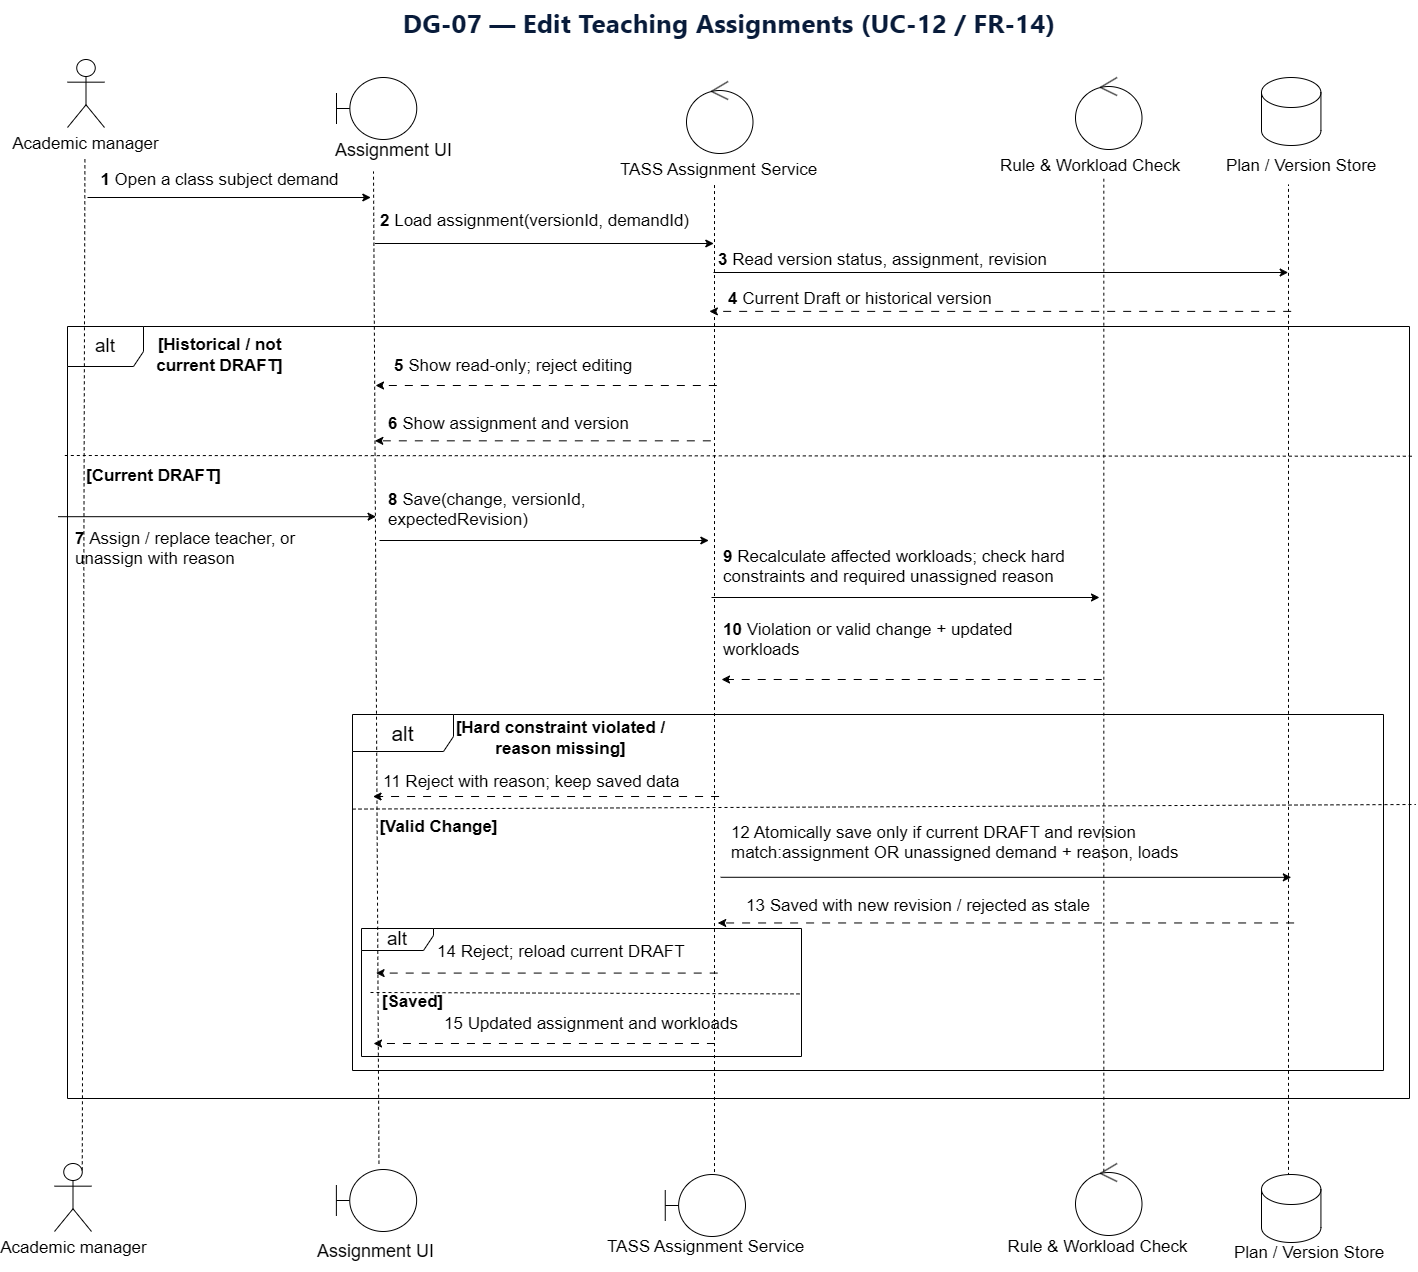
\includegraphics[width=0.98\linewidth,height=0.63\textheight,keepaspectratio]{diagrams/DG-07.png}
\caption{DG-07 --- Tuần tự chỉnh sửa phân công}\label{fig:DG-07}
\end{figure}

\diagramtext{Khung rẽ nhánh (alt) đầu phân biệt bản lịch sử/chưa phải DRAFT hiện hành với bản được phép sửa. Với DRAFT hiện hành, dịch vụ tính lại tải và kiểm tra điều kiện cứng, sau đó chỉ lưu trong một giao dịch nguyên tử nếu revision vẫn khớp. Yêu cầu lỗi hoặc đã cũ được trả lại để sửa/tải bản hiện hành; khi bỏ gán, nhu cầu và lý do vẫn được giữ theo FR-14 và NFR-04.}


Hình~\ref{fig:DG-08} trình bày luồng UC-18--20 từ khi Teacher gửi phản hồi đến khi Academic Manager xử lý và xuất đề xuất. Chuỗi thông điệp làm rõ phiên bản nguồn của phản hồi, bước tạo phiên bản tiếp theo và điểm kiểm tra trước khi phát hành PDF.

\begin{figure}[H]
\centering
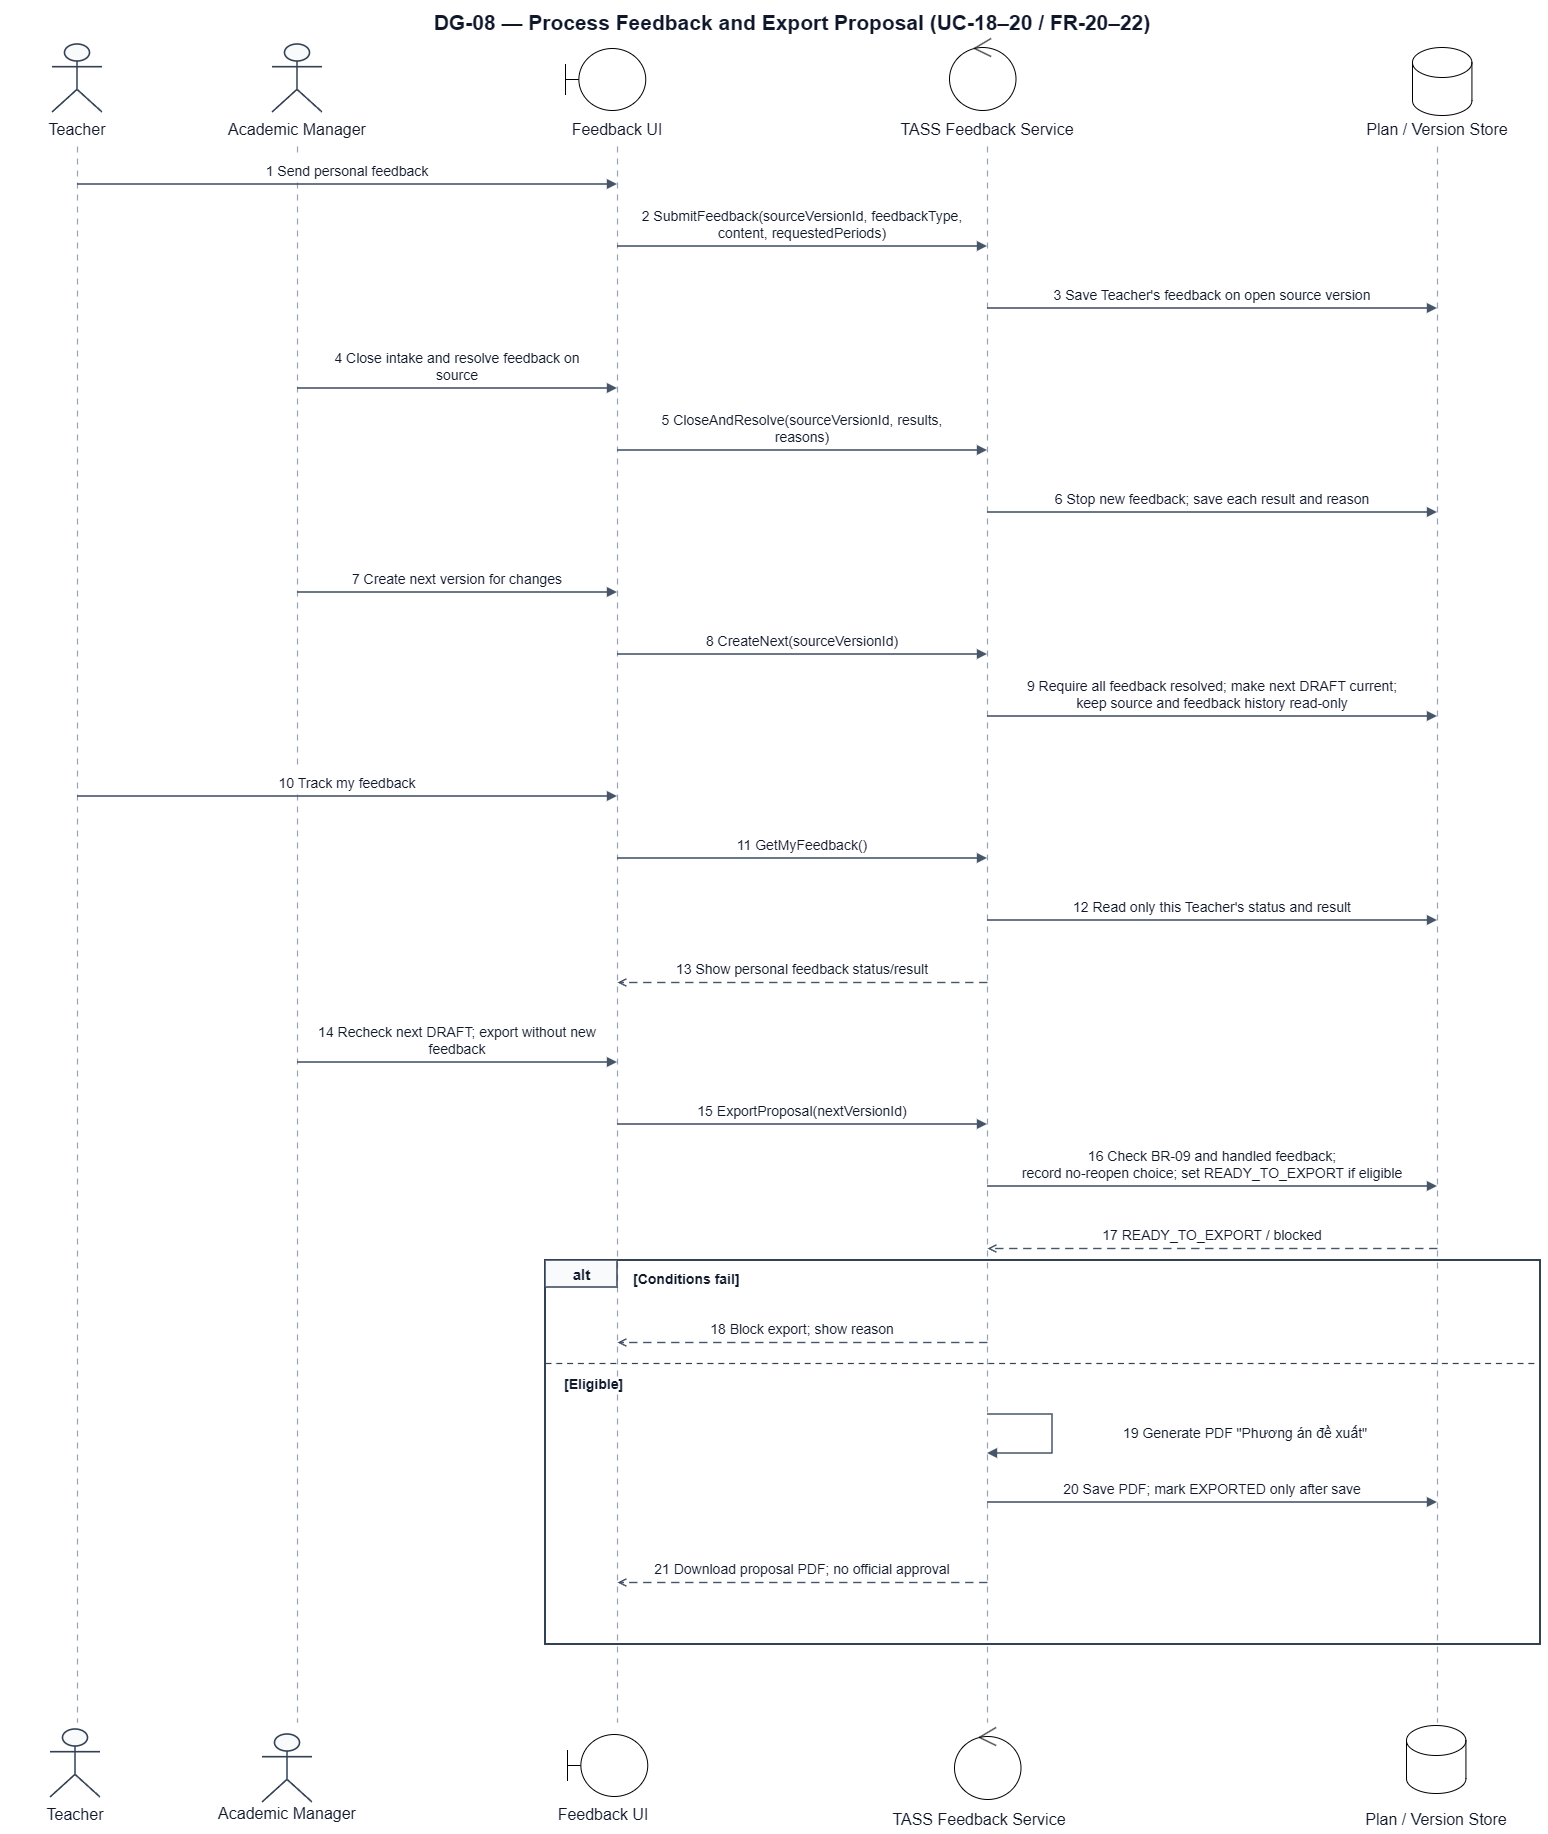
\includegraphics[width=0.98\linewidth,height=0.68\textheight,keepaspectratio]{diagrams/DG-08.png}
\caption{DG-08 --- Tuần tự xử lý phản hồi và xuất đề xuất}\label{fig:DG-08}
\end{figure}

\diagramtext{Nhánh tạo DRAFT mới áp dụng khi cần đổi gán; nguồn và phản hồi đã gửi được giữ lịch sử. Trường requestedPeriods là tổng tiết mong muốn của môn theo FR-20, không phải phần tăng. Nhánh xuất không mở lại chỉ được đi tiếp khi Academic Manager ghi nhận lựa chọn đó, xử lý xong phản hồi và đạt BR-09. Hệ thống chỉ ghi EXPORTED sau khi lưu PDF thành công; tệp xuất vẫn là phương án đề xuất theo FR-22.}

\section{Giải thích nhu cầu chưa phân công}
CP-SAT cho biết $y_j=1$, không tự trả nguyên nhân nghiệp vụ đầy đủ.
\begin{longtable}{|p{5cm}|p{8.9cm}|}\hline
Mã / phạm vi & Nghĩa và giới hạn kết luận \\\hline\endfirsthead
\hline Mã / phạm vi & Nghĩa và giới hạn kết luận \\\hline\endhead
\code{NO_QUALIFIED_TEACHER} & Không có ứng viên đã xác nhận đủ điều kiện trong bản chụp dữ liệu/phạm vi đang xét; liệt kê hồ sơ chưa xác nhận nếu có, không kết luận trường không thể bổ sung người. \\\hline
\code{CAPACITY_EXCEEDED} & Không gán thêm trực tiếp được vào phương án hiện tại vì giới hạn tải đã kiểm tra. Chưa chứng minh không có cách đổi các gán khác để phủ nhu cầu. Muốn kết luận bất khả thi toàn cục cần lượt kiểm tra bổ sung có chứng minh. \\\hline
\code{LOCK_CONFLICT} & Khóa mâu thuẫn, giáo viên không hợp lệ hoặc khóa vượt giới hạn; từ chối và giữ DRAFT, chỉ rõ khóa/ràng buộc liên quan. \\\hline
\code{MISSING_INPUT} & Kết quả tiền kiểm khi thiếu đầu vào bắt buộc; không tự đưa nhu cầu thiếu số tiết vào nghiệm hợp lệ. Thiếu dữ liệu năm là kết quả kiểm tra năm riêng. \\\hline
\code{TIME_LIMIT} & Nguyên nhân kết thúc do chạm ngưỡng ngân sách thời gian của lượt chạy/giai đoạn giải thuật; không được tự ý gán đây là nguyên nhân chuyên môn của từng nhu cầu chưa được phân công. \\\hline
\code{MANUALLY_UNASSIGNED} & Người quản lý chủ động bỏ gán kèm lý do; đây không phải khóa giữ trống cho lần tối ưu sau. \\\hline
\end{longtable}
Nếu chưa có đủ căn cứ, kết quả phải ghi rõ nguyên nhân chưa được xác định đầy đủ, cùng mã chẩn đoán, dữ liệu và mức bảo đảm. Bộ kiểm tra xác nhận sự phù hợp của một phương án với các ràng buộc; việc này không thay thế chứng minh tối ưu hoặc chứng minh mô hình vô nghiệm.

\chapter{KIỂM CHỨNG VÀ ĐÁNH GIÁ}\label{chap:verification}
Việc đánh giá được thực hiện theo ba lớp: tiêu chí cần kiểm chứng, mức độ hiện thực trong mã nguồn và kết quả thực nghiệm đã thu thập. Cách trình bày này phân biệt yêu cầu thiết kế với những kết luận đã có bằng chứng.


\section{Phạm vi và tiêu chí nghiệm thu}\label{sec:acceptance}
Quá trình kiểm chứng sử dụng bản chụp E3 năm học 2026--2027 trong phạm vi THCS và THPT, đồng thời ghi nhận số giáo viên, số nhu cầu sau chuẩn hóa và các đối tượng được loại khỏi phạm vi. Bộ giải phải tuân thủ ràng buộc cứng, tính đúng tải và đơn vị, bảo toàn các phân công bị khóa, bản chụp dữ liệu và nghiệm khả thi đã tìm được khi xảy ra lỗi, hủy tác vụ hoặc xung đột cập nhật. Kết quả chẩn đoán phải nêu đúng mức bảo đảm; độ phủ tối đa chỉ được xác nhận bằng chứng minh tối ưu hoặc kết quả đối chiếu độc lập. Phương án OPTIMAL nhưng chưa phân công đủ nhu cầu vẫn phải tuân BR-09.

Các bảng T và POC trình bày kế hoạch kiểm chứng, còn kết quả thực nghiệm đã thu thập được trình bày tại Mục~\ref{sec:historical-results}. Việc định nghĩa cấu trúc dữ liệu trong mã nguồn chưa đủ để xác nhận chức năng tương ứng đã vượt qua kiểm thử nghiệm thu trên E3.

\section{Truy vết FR--UC--BR--test}\label{sec:traceability}

\begin{longtable}{|p{2.3cm}|p{2.4cm}|p{6.7cm}|p{1.5cm}|}
\hline
\textbf{FR} & \textbf{UC} & \textbf{BR chính} & \textbf{Test} \\\hline
\endfirsthead
\hline
\textbf{FR} & \textbf{UC} & \textbf{BR chính} & \textbf{Test} \\\hline
\endhead
FR-01 & UC-01 & BR-14 & T-01 \\\hline
FR-02--03 & UC-02 & BR-14 & T-02 \\\hline
FR-04 & UC-03 & BR-02, BR-14 & T-03 \\\hline
FR-05 & UC-04 & BR-01 & T-04 \\\hline
FR-06 & UC-05 & BR-03, BR-08 & T-05 \\\hline
FR-07 & UC-06 & BR-14 & T-06 \\\hline
FR-08 & UC-07 & BR-01, BR-09, BR-12 & T-07 \\\hline
FR-09 & UC-08 & BR-04--06 & T-08 \\\hline
FR-12 & UC-17 & BR-11, BR-14, BR-22 & T-11 \\\hline
FR-13 & UC-11 & BR-10, BR-14, BR-22 & T-12 \\\hline
FR-14 & UC-12 & BR-01--03, BR-06, BR-15, BR-22 & T-13 \\\hline
FR-15 & UC-13 & BR-01--08, BR-15, BR-22 & T-14 \\\hline
FR-16 & UC-14 & BR-01--09, BR-15 & T-15 \\\hline
FR-17 & UC-15 & BR-04--07 & T-16 \\\hline
FR-18 & UC-15 & BR-05--07, BR-15, BR-22 & T-17 \\\hline
FR-19 & UC-16 & BR-09, BR-14, BR-22 & T-18 \\\hline
FR-20 & UC-18 & BR-06, BR-11, BR-14 & T-19 \\\hline
FR-21 & UC-19 & BR-09--10, BR-14, BR-22 & T-20 \\\hline
FR-22 & UC-20 & BR-09, BR-14, BR-22 & T-21 \\\hline
FR-23 & UC-21 & BR-10, BR-14 & T-22 \\\hline
\end{longtable}


\section{Ca kiểm chứng Solver và dữ liệu}\label{sec:solver-tests}

\begin{longtable}{|p{1.6cm}|p{12.3cm}|}
\hline
\textbf{Mã} & \textbf{Tình huống và kết quả cần kiểm chứng} \\\hline
\endfirsthead
\hline
\textbf{Mã} & \textbf{Tình huống và kết quả cần kiểm chứng} \\\hline
\endhead
POC-01 & Bộ nhỏ có phương án đầy đủ tối ưu biết trước: gán đúng, bộ kiểm tra không có vi phạm cứng trên phạm vi đủ dữ liệu. \\\hline
POC-02 & Nhiều nghiệm có điểm tối ưu đã tính độc lập: khi chứng minh OPTIMAL thì khớp điểm; nếu FEASIBLE chỉ khẳng định khả thi và ghi bound. \\\hline
POC-03 & Không có ứng viên đã xác nhận: để trống và báo đúng phạm vi nguyên nhân, không gán sai chuyên môn. \\\hline
POC-04 & Ứng viên không còn tải: không ép gán; chẩn đoán phân biệt giới hạn trên nghiệm hiện tại và bất khả thi đã chứng minh. \\\hline
POC-05 & Tính đúng B/R/Q/F/C/A/W/T và lệch T-B theo bộ dữ liệu minh họa; đúng đơn vị và hiệu lực/biểu thức giới hạn, không đếm trùng. \\\hline
POC-06 & Khóa hợp lệ được giữ nguyên qua cả năm bước và chạy lại; không đếm hai lần trong F/A. \\\hline
POC-07 & Khóa xung đột hoặc không còn hợp lệ: trả LOCK\_CONFLICT, không bỏ khóa hoặc ghi đè DRAFT. \\\hline
POC-08 & Dừng trước khi chứng minh tối ưu: nếu có nghiệm thì giữ nghiệm khả thi/metadata; nếu chưa có nghiệm thì không đọc biến. Không ép một bộ nhỏ luôn phải ra FEASIBLE chỉ bằng timeout rất ngắn. \\\hline
POC-09 & Hủy ở tầng ứng dụng nếu có hỗ trợ: giữ dữ liệu đã lưu, không áp dụng kết quả đến sau hủy. Không dùng CANCELLED như trạng thái CP-SAT. \\\hline
POC-10 & Chạy lại trong cùng đợt và học kỳ: giữ gán có khóa; gán tự động chưa khóa được đổi để cải thiện mục tiêu trước, tính Echg ở bước 5. Không có phương án làm mốc thì Echg=0; không tự so sánh hai học kỳ. Lịch sử không đổi. \\\hline
POC-11 & Tiết lẻ và tích quy đổi: đổi đơn vị chính xác, không cắt số; giá trị chưa biết không trở thành 0. \\\hline
POC-12 & Tải ngoài phạm vi và nguồn năm: không đếm trùng giữa F/A/C hoặc các phương án thay thế. \\\hline
POC-13 & B=(10,10), tải (10,0) và (5,5): L1 cùng 10 nhưng M là 10 và 5; chọn M nhỏ hơn sau cố định Z/L1. \\\hline
POC-14 & Bước sau không tìm thấy nghiệm mới: giữ nghiệm khả thi tốt nhất đã tìm được trước. Bước 5 OPTIMAL không chứng minh Z/L1/M/Eexp tối ưu nếu các bước tương ứng chưa có bằng chứng. \\\hline
POC-15 & Trong lúc chạy có sửa DRAFT/đổi dữ liệu/chuyển phiên bản: không áp dụng kết quả cũ. \\\hline
POC-16 & Thiếu dữ liệu bắt buộc: dừng tiền kiểm. Thiếu riêng dữ liệu năm: giữ INSUFFICIENT\_DATA và chính sách BR-09. \\\hline
POC-17 & Ba loại thành phần không trùng/thiếu; chuẩn và chuyên đề được cùng hoặc khác giáo viên, giữ đúng khóa gán. \\\hline
POC-18 & Hai học kỳ/công tác/nghỉ toàn kỳ: xét đúng semester và hiệu lực; không gán người nghỉ, không phạt thiếu tải không áp dụng. \\\hline
POC-19 & Phản hồi tăng tải dùng tổng môn trên nguồn; không tự thêm nhu cầu; thay đổi tạo DRAFT mới và nguồn giữ lịch sử. \\\hline
POC-20 & Mở/xuất: chặn DRAFT thiếu, kiểm tra cũ hoặc vi phạm; thiếu năm chỉ cảnh báo theo BR-09; lỗi PDF không ghi EXPORTED. \\\hline
POC-21 & Nhãn nguồn A1+A2 được chuẩn hóa thành hai nhu cầu riêng, mỗi lớp 1 tiết: hai thành phần, cùng giáo viên thì tổng tải 2 tiết. Không tạo một nhu cầu dùng chung trong demo. \\\hline
POC-22 & KHTN của một lớp được lưu toàn môn và giao cho một giáo viên có qualification KHTN còn hiệu lực. Không tách thành Lý/Hóa/Sinh, không suy quyền dạy toàn môn từ một môn riêng và không cộng tải toàn môn với tải chi tiết. \\\hline
POC-23 & Kiểm thứ tự Z/L1/M/experience/change bằng bộ đối chiếu độc lập: kinh nghiệm không làm xấu Z/L1/M; với cùng Z/L1/M, chọn Eexp nhỏ hơn kể cả khi tăng số thay đổi của gán chưa khóa; chỉ tối thiểu Echg khi Eexp bằng nhau. \\\hline
POC-24 & Kiểm kinh nghiệm theo số năm/môn/khối và trọng số khối 9/12; phân biệt số năm 0 với chưa biết, không cộng trùng thời gian dạy nhiều lớp. Đầu vào nhu cầu vượt hai chữ số thập phân phải bị từ chối trước ghi DB. Kiểm đơn vị/scale, dòng tổng/thành phần, 2+1*, 0/2, tt và TH theo Mục~\ref{sec:excel}. \\\hline
\end{longtable}


\begin{longtable}{|p{2.3cm}|p{11.6cm}|}
\hline
\textbf{Mã bổ sung} & \textbf{Điểm kiểm chứng và liên hệ} \\\hline
\endfirsthead
\hline
\textbf{Mã bổ sung} & \textbf{Điểm kiểm chứng và liên hệ} \\\hline
\endhead
T-XL-01 & Giữ file/sheet/ô, ID/bí danh và nguồn mâu thuẫn để đối soát; không tự hợp nhất/lấy 0 (FR-04/05/08). \\\hline
T-XL-02 & Chuyên đề A1+A2 tách thành nhu cầu 12A1 và 12A2; mỗi lớp 1 tiết thì giáo viên dạy cả hai nhận 2 tiết. Giữ nhãn nguồn, đối soát từng lớp và không tạo dòng dùng chung (POC-21). \\\hline
T-XL-03 & Dòng 57: A=12,R=8,B=17 cho T=20,Q=9,W=12, T-B=W-Q=3; không thêm 8 vào C (POC-05). \\\hline
T-XL-04 & Các ví dụ Mục~\ref{sec:excel} khớp phép tính thập phân/scale, không cộng lại dòng tổng (POC-11/24). \\\hline
T-ALG-21 & Mỗi bước lưu trạng thái, giá trị mục tiêu, cận, bằng chứng tối ưu và định danh bản chụp cùng cấu hình. Nếu bước sau không có nghiệm mới, hệ thống giữ nghiệm trước; khi UNKNOWN không có nghiệm, hệ thống không đọc biến (POC-08/14). \\\hline
T-ALG-22 & Ngân sách 60 giây đo toàn lượt, không 60 giây mỗi bước; phân biệt solve() với HTTP/queue/database (NFR-03). \\\hline
T-ALG-23 & Báo thiếu thành phần/tiết/nhóm, chỉ kết luận thiếu tối thiểu khi có bằng chứng tối ưu; so mục tiêu cùng coverage/config/scale. \\\hline
T-ALG-24 & Chặn mở lấy ý kiến hoặc xuất tài liệu khi thiếu gán/tuần, vi phạm hoặc kiểm tra cũ; thiếu riêng năm cảnh báo theo BR-09 (POC-20). \\\hline
\end{longtable}


\section{Mức độ hiện thực}\label{sec:implementation-audit}
Các nhận xét về solver Java trong bảng dựa trên rà soát ngày 31/10/2026, cần đối chiếu lại trước nghiệm thu phiên bản hiện hành. Phần lưu trữ được cập nhật bằng đối chiếu tĩnh ERD/SQL ngày 09/11/2026; chưa chạy bộ SQL mới trong lần biên tập này. Việc có cấu trúc lưu trữ không đồng nghĩa đã hoàn tất API hoặc tích hợp thuật toán.

\begin{longtable}{|p{3.7cm}|p{10.2cm}|}
\hline
\textbf{Truy vết} & \textbf{Kết quả rà soát} \\\hline
\endfirsthead
\hline
\textbf{Truy vết} & \textbf{Kết quả rà soát} \\\hline
\endhead
FR-08; DATA-04/06; HC-01/02 & Có Demand đơn classId, qualification subjectId/levelId; còn thiếu ENRICHMENT. Cần chuẩn hóa đầu vào KHTN nguyên môn và kiểm tra qualification tương ứng. ModelBuilder/SolutionValidator và HeuristicProblem còn ép cùng giáo viên giữa các thành phần; cần bỏ chính sách chung này theo BR-01. Nhóm ghép và quan hệ môn cha/phân môn không còn là phần thiếu của MVP. \\\hline
FR-17; BR-04/16; DATA-16 & Có B/R/Q/F/C/A/W, BigDecimal/scale, targetApplicable, FULL\_TERM\_LEAVE và Precheck/HardCheck từ đầu vào; thiếu T/B trong kết quả, bộ tính 5 nhóm/tải năm 18/17 và bản chụp dữ liệu E3 đầy đủ. Chuẩn hóa ký hiệu workbook chưa hiện thực. \\\hline
FR-15; SC-01--04 & Có COMPONENTS và ba thuật toán; AssignmentSolver còn COVERAGE/SOFT, chưa thực hiện thứ tự năm bước Z/L1/M/experience/change. Cần bổ sung M, điểm kinh nghiệm có trọng số khối 9/12 và đồng bộ tiền kiểm theo cấu hình hiện hành. \\\hline
FR-14; HC-04 & DDL mới đã có is\_locked, dấu vết khóa và guard phân công. Ở PoC được rà soát trước đây, previousAssignments chỉ góp điểm thay đổi; còn cần đối chiếu DTO/ràng buộc solver và nối đồng bộ với API, UI, quyền cùng bộ kiểm tra. \\\hline
NFR-03/04; DATA-18 & Có fallback/status/bound và budget trong solve(); chưa chứng minh năm bước, toàn lượt HTTP/queue/database và chống kết quả cũ trong sản phẩm. \\\hline
FR-19--22; DATA-09/12 & AssignmentService/store bộ nhớ là mô phỏng; chưa có bằng chứng đầy đủ web/database/PDF. ID/bộ dữ liệu kiểm thử E3 chưa hoàn chỉnh. ERD và DDL 48 bảng đã cập nhật ngày 08/11/2026; bộ SQL có seed/query minh họa, còn cần đồng bộ backend và kiểm thử tích hợp theo Mục~\ref{sec:future-work}. \\\hline
\end{longtable}


\section{Kết quả thực nghiệm đã thu thập}\label{sec:historical-results}
Bộ kết quả tại \code{tass-comparison/results/verified-comparison/} gồm các tệp runs.csv, summary.csv và manifest.json, với 4 bộ dữ liệu kiểm thử $\times$ 5 lượt $\times$ 3 thuật toán = 60 lượt. Các thuật toán sử dụng cùng inputHash cho mỗi cặp dữ liệu và lượt chạy. Số liệu được thu thập từ phiên bản PoC trước đây, sử dụng hai giai đoạn COVERAGE và SOFT cùng ràng buộc bắt buộc một giáo viên phụ trách các thành phần của cùng nhóm. Vì vậy, kết quả này chưa đánh giá khóa phân công hoặc quy trình tối ưu năm bước của thiết kế hiện hành.

Theo manifest, môi trường thử nghiệm gồm Windows 11 amd64, Temurin 21.0.12.1+1-LTS, 16 bộ xử lý logic, OR-Tools 9.14.6206 và một luồng tìm kiếm (worker). Mỗi lượt có giới hạn 2 giây, với một lượt khởi động thử (warm-up) cho mỗi thuật toán. GA sử dụng quần thể 40 cá thể, xác suất đột biến 0.1 và tối đa 200 thế hệ; CP-SAT phiên bản cũ dành tối đa 45\% thời gian cho mỗi giai đoạn. Phép đo solve() bao gồm kiểm tra đầu vào và nghiệm, nhưng chưa bao gồm đọc JSON, khởi động JVM, HTTP, hàng đợi hoặc giao dịch cơ sở dữ liệu. Việc đối soát các tệp CSV chỉ xác nhận tính nhất quán của số liệu đã lưu, không xác nhận mã nguồn hiện tại giống hoàn toàn mã tại thời điểm chạy.

Trong bảng kết quả, cột ``Thiếu'' biểu thị trung vị của số thành phần chưa được phân công. Các thời gian được tính bằng mili giây và làm tròn đến ba chữ số thập phân. Với mẫu năm lượt và cách lấy hạng gần nhất, p95 trong bảng là giá trị lớn nhất của mẫu.
\begin{longtable}{|p{3.2cm}|p{1.7cm}|p{1.4cm}|p{1.4cm}|p{1.7cm}|p{1.7cm}|}\hline
Bộ dữ liệu kiểm thử và thuật toán & Hợp lệ & Phủ đủ & Thiếu & Median ms & p95 ms \\\hline\endfirsthead
\hline Bộ dữ liệu kiểm thử và thuật toán & Hợp lệ & Phủ đủ & Thiếu & Median ms & p95 ms \\\hline\endhead
component-consistency / GREEDY & 5/5 & 0/5 & 1 & 3.506 & 6.730 \\\hline
component-consistency / GENETIC & 5/5 & 0/5 & 1 & 36.480 & 57.105 \\\hline
component-consistency / CP\_SAT & 5/5 & 0/5 & 1 & 10.903 & 11.357 \\\hline
decimal-load / GENETIC & 5/5 & 5/5 & 0 & 42.354 & 59.433 \\\hline
decimal-load / CP\_SAT & 5/5 & 5/5 & 0 & 7.582 & 8.288 \\\hline
decimal-load / GREEDY & 5/5 & 5/5 & 0 & 1.779 & 2.693 \\\hline
greedy-trap / CP\_SAT & 5/5 & 5/5 & 0 & 5.787 & 7.947 \\\hline
greedy-trap / GREEDY & 5/5 & 5/5 & 0 & 1.641 & 2.363 \\\hline
greedy-trap / GENETIC & 5/5 & 5/5 & 0 & 15.252 & 19.832 \\\hline
shortage / GREEDY & 5/5 & 0/5 & 1 & 1.389 & 1.959 \\\hline
shortage / GENETIC & 5/5 & 0/5 & 1 & 13.171 & 14.357 \\\hline
shortage / CP\_SAT & 5/5 & 0/5 & 1 & 6.294 & 11.492 \\\hline
\end{longtable}
Cả ba thuật toán đều tạo phương án hợp lệ trong 20/20 lượt và phân công đầy đủ trong 10/20 lượt, với cùng độ phủ trên từng bộ dữ liệu. Tại mức độ phủ tốt nhất, điểm mềm là 100 cho component-consistency và 0 cho ba bộ dữ liệu còn lại theo cùng cấu hình. CP-SAT cung cấp bằng chứng tối ưu về độ phủ trong 20/20 lượt, còn Greedy và GA không cung cấp bằng chứng này trong các lượt thử đã ghi nhận. Điều đó không có nghĩa các phương án do Greedy và GA tìm được có chất lượng thấp hơn. Trên hai bộ dữ liệu thiếu giáo viên, mỗi thuật toán phân công được 1/2 số nhu cầu; bằng chứng của CP-SAT xác nhận đây là mức thiếu nhỏ nhất của mô hình cũ, chứ chưa xác nhận phương án đủ điều kiện mở lấy ý kiến hoặc xuất tài liệu.

Trên cả bốn bộ dữ liệu, Greedy có thời gian trung vị ngắn nhất, tiếp theo là CP-SAT và GA. Bộ thử nghiệm này chưa cho thấy CP-SAT tạo phương án có chất lượng cao hơn hai thuật toán đối chứng; ưu điểm được ghi nhận là khả năng cung cấp bằng chứng tối ưu. Do số lượt còn ít và phạm vi đo chỉ bao gồm solve(), kết quả chưa đủ để xác nhận NFR-03 trên quy mô dữ liệu nhà trường.

\section{Kế hoạch đánh giá mô hình hiện hành}
Kế hoạch đánh giá mô hình hiện hành sử dụng các bài toán nhỏ có kết quả đối chiếu độc lập, bản chụp E3 đã ẩn danh và dữ liệu tổng hợp cho ba nhóm: đủ giáo viên, thiếu giáo viên và giới hạn tải gần ngưỡng. Cả ba thuật toán phải sử dụng cùng dữ liệu và mã băm, bộ quy tắc, hệ số tỷ lệ, mục tiêu, phân công trước đó, khóa, giới hạn thời gian và bộ kiểm tra. Các cấu trúc dữ liệu, mô hình và bộ kiểm tra phải được đồng bộ trước khi đánh giá KHTN nguyên môn, nhu cầu riêng từng lớp, kinh nghiệm và khóa phân công.

Mỗi thuật toán được khởi động thử riêng và thứ tự chạy được luân phiên; hồ sơ thử nghiệm ghi cấu hình máy, phiên bản, tệp JAR, mã băm, hạt giống ngẫu nhiên (seed) và số worker. Nhóm đề xuất trao đổi với GVHD về việc chạy ít nhất 30 lượt cho mỗi nhóm dữ liệu, với các giới hạn 2, 10 và 60 giây; NFR-03 được đo trên toàn bộ quy trình. Các chỉ số gồm tỷ lệ phương án hợp lệ và phân công đủ, số thành phần hoặc tiết còn thiếu, cặp lớp--môn chưa hoàn chỉnh, Eload/M/Eexp/Echg; thời gian tìm nghiệm đầu tiên, trung vị, p95, bộ nhớ, số biến và ràng buộc, giá trị mục tiêu, cận và bằng chứng của từng bước, cùng số lượt vượt thời gian. Lượt không tìm được nghiệm phải được ghi nhận riêng, thay vì gán điểm chất lượng bằng 0. Cùng seed không bảo đảm cùng nghiệm hoặc thời gian trên mọi môi trường.

Đối với bài toán cực tiểu, có thể báo cáo $gap_{abs}=f-b$ và $gap_{rel}=(f-b)/\max(1,|f|)$, trong đó f là giá trị của nghiệm khả thi tốt nhất đã tìm được và b là cận dưới, được tính theo cùng đơn vị. Quy ước báo cáo này không thay thế ngưỡng dừng của bộ giải. Việc so sánh với phương án Excel chỉ có ý nghĩa khi sử dụng cùng nhu cầu và quy tắc; phương án lịch sử không mặc nhiên là phương án tối ưu.

\chapter{CÔNG VIỆC CẦN HOÀN THIỆN}\label{chap:decisions}
Chương này tổng hợp các công việc cần hoàn thiện trước khi nghiệm thu và hướng mở rộng sau MVP. Các quyết định nghiệp vụ đã thống nhất được thể hiện trực tiếp trong các chương đặc tả và mô hình thuật toán; ưu tiên kinh nghiệm được quy định tại BR-08 và Mục~\ref{sec:objectives}.

\section{Hướng hoàn thiện}\label{sec:future-work}
Các hạng mục chưa hoàn thành được tổng hợp tại Mục~\ref{sec:implementation-audit} và cần được kiểm chứng theo Chương~\ref{chap:verification} trước khi ghi nhận đạt yêu cầu. Trọng tâm tiếp theo là đồng bộ bộ SQL 48 bảng với các lớp dữ liệu và API, hoàn thiện tích hợp solver và chuẩn hóa dữ liệu E3. Bộ schema, seed và Q01--Q32 cần được chạy trên PostgreSQL thử nghiệm, bổ sung kiểm thử tích hợp và trình GVHD rà soát thiết kế hiện hành.

Ở tầng dịch vụ, cần hoàn thiện phân quyền, kiểm tra tải và kiểm soát phiên bản, revision, snapshot cùng token nguồn trong giao dịch. Các ca kiểm thử cần bao phủ cập nhật đồng thời, kết quả solver về muộn, khóa phân công và phản hồi quá hạn. Luồng xuất PDF phải tạo và lưu tệp thành công trước khi ghi nhận xuất; kiểm thử cần xác nhận việc chặn dữ liệu cũ, vi phạm hoặc thiếu dữ liệu tuần, đồng thời giữ cảnh báo khi chỉ thiếu dữ liệu năm theo BR-09.

Sau MVP, hệ thống có thể mở rộng các chế độ đặc thù, thỉnh giảng, thẩm định chế độ và tích hợp với phần mềm bên ngoài.

Nhóm lớp ghép và tính tải dùng chung cho nhiều lớp (nội dung ERD-02 trước đây) nằm ngoài demo. Khi phát triển chức năng này, cần một mô hình nhóm/thành viên và nhu cầu dùng chung, đồng thời đối soát lại dữ liệu để tránh cộng tải trùng. Phân công KHTN theo từng mạch nội dung cũng là hướng mở rộng nếu phạm vi trường áp dụng yêu cầu; mô hình một giáo viên dạy toàn môn hiện tại là lựa chọn cho demo, không phải kết luận mọi trường đều tổ chức giống nhau.

Việc mở rộng sang thời khóa biểu cần một mô hình riêng cho ngày, tiết học và phòng học, với các ràng buộc về trùng giáo viên, lớp hoặc phòng, thời gian khả dụng, di chuyển và phân bố tiết trong tuần. Kết quả phân công hiện tại chỉ là đầu vào đề xuất. Nếu không xây dựng được lịch phù hợp, hệ thống cần cơ chế phản hồi để điều chỉnh phân công; tính hợp lệ về tải chưa bảo đảm luôn tồn tại một thời khóa biểu khả thi.
\chapter*{TÀI LIỆU THAM KHẢO}
\phantomsection\addcontentsline{toc}{chapter}{TÀI LIỆU THAM KHẢO}\label{chap:references}
\begin{enumerate}[label={[\arabic*]},leftmargin=1.1cm,itemsep=0.6em]
\item\label{ref:source-1} Luật Giáo dục số 43/2019/QH14; \href{https://vanban.chinhphu.vn/?docid=216504\&pageid=27160}{Luật số 123/2025/QH15 sửa đổi, bổ sung một số điều của Luật Giáo dục}; \href{https://vanban.chinhphu.vn/?docid=217346\&pageid=27160}{Văn bản hợp nhất số 72/VBHN-VPQH về Luật Giáo dục}.

\item\label{ref:source-2} \href{https://vanban.chinhphu.vn/?docid=214559\&pageid=27160}{Luật Nhà giáo số 73/2025/QH15}.

\item\label{ref:source-3} \href{https://vanban.chinhphu.vn/?docid=217499\&pageid=27160}{Nghị định số 93/2026/NĐ-CP quy định chi tiết và hướng dẫn thi hành một số điều của Luật Nhà giáo}.

\item\label{ref:source-4} \href{https://vanban.chinhphu.vn/?docid=213113\&pageid=27160}{Thông tư số 05/2025/TT-BGDĐT quy định chế độ làm việc đối với giáo viên phổ thông, dự bị đại học}.

\item\label{ref:source-5} \href{https://vanban.chinhphu.vn/?docid=216931\&pageid=27160}{Thông tư số 04/2026/TT-BGDĐT quy định chế độ làm việc đối với giáo viên cơ sở giáo dục thường xuyên}.

\item\label{ref:source-6} \href{https://vanban.chinhphu.vn/?docid=208996\&pageid=27160}{Thông tư số 20/2023/TT-BGDĐT hướng dẫn về vị trí việc làm, cơ cấu viên chức theo chức danh nghề nghiệp và định mức số lượng người làm việc trong các cơ sở giáo dục phổ thông và các trường chuyên biệt công lập}.

\item\label{ref:source-7} \href{https://vanban.chinhphu.vn/?docid=184806\&pageid=27160}{Thông tư số 08/2016/TT-BGDĐT quy định chế độ giảm định mức giờ dạy cho giáo viên, giảng viên làm công tác công đoàn không chuyên trách trong các cơ sở giáo dục công lập thuộc hệ thống giáo dục quốc dân}.

\item\label{ref:source-8} \href{https://vanban.chinhphu.vn/?docid=165723\&pageid=27160}{Quyết định số 13/2013/QĐ-TTg về chế độ, chính sách đối với cán bộ Đoàn Thanh niên Cộng sản Hồ Chí Minh, Hội Sinh viên Việt Nam, Hội Liên hiệp Thanh niên Việt Nam trong các cơ sở giáo dục và cơ sở dạy nghề}.

\item\label{ref:source-9} \href{https://vanban.chinhphu.vn/?docid=215347\&pageid=27160}{Thông tư số 17/2025/TT-BGDĐT sửa đổi, bổ sung một số nội dung trong Chương trình giáo dục phổ thông ban hành kèm theo Thông tư số 32/2018/TT-BGDĐT}.

\item\label{ref:source-10} \href{https://vanban.chinhphu.vn/?docid=201098\&pageid=27160}{Thông tư số 32/2020/TT-BGDĐT ban hành Điều lệ trường trung học cơ sở, trường trung học phổ thông và trường phổ thông có nhiều cấp học}.

\item\label{ref:source-11} \href{https://vanban.chinhphu.vn/?docid=215462\&pageid=27160}{Thông tư số 21/2025/TT-BGDĐT quy định chế độ trả tiền lương dạy thêm giờ đối với nhà giáo trong các cơ sở giáo dục công lập}.

\item\label{ref:source-12} \href{https://thuvienphapluat.vn/cong-van/Giao-duc/Cong-van-5636-BGDDT-GDTrH-2023-xay-dung-ke-hoach-day-hoc-cac-mon-hoc-Khoa-hoc-tu-nhien-584066.aspx}{Công văn số 5636/BGDĐT-GDTrH về xây dựng kế hoạch dạy học các môn Khoa học tự nhiên, Lịch sử và Địa lí, Hoạt động trải nghiệm, hướng nghiệp}.

\item\label{ref:source-13} \href{https://xaydungchinhsach.chinhphu.vn/cong-van-so-5555-bgddt-gdpt-huong-dan-to-chuc-hoat-dong-cua-truong-mam-non-pho-thong-sau-sap-xep-119260819092236042.htm}{Công văn số 5555/BGDĐT-GDPT hướng dẫn tổ chức, hoạt động của trường mầm non, phổ thông sau sắp xếp}.

\item\label{ref:source-14} \href{https://thuvienphapluat.vn/cong-van/Giao-duc/Cong-van-5243-BGDDT-NGCBQLGD-2026-quan-ly-doi-ngu-nha-giao-can-bo-quan-ly-co-so-giao-duc-718885.aspx}{Công văn số 5243/BGDĐT-NGCBQLGD hướng dẫn thực hiện công tác quản lý đội ngũ nhà giáo, cán bộ quản lý cơ sở giáo dục và nhân sự hỗ trợ giáo dục}.

\item\label{ref:source-15} \href{https://vanban.chinhphu.vn/?docid=217839\&pageid=27160}{Thông tư số 30/2026/TT-BGDĐT quy định chuẩn nghề nghiệp giáo viên cơ sở giáo dục phổ thông}.

\item\label{ref:source-16} \href{https://vanban.chinhphu.vn/?docid=217840\&pageid=27160}{Thông tư số 31/2026/TT-BGDĐT quy định mã số, bổ nhiệm chức danh và xếp lương đối với nhà giáo trong cơ sở giáo dục công lập}.

\item\label{ref:source-17} \href{https://vanban.chinhphu.vn/?docid=214590\&pageid=27160}{Luật Bảo vệ dữ liệu cá nhân số 91/2025/QH15}.

\item\label{ref:source-18} \href{https://vanban.chinhphu.vn/?docid=216387\&pageid=27160}{Nghị định số 356/2025/NĐ-CP quy định chi tiết một số điều và biện pháp thi hành Luật Bảo vệ dữ liệu cá nhân}.

\item\label{ref:source-19} \href{https://vanban.chinhphu.vn/?docid=212488\&pageid=27160}{Luật Dữ liệu số 60/2024/QH15}.

\item\label{ref:source-20} \href{https://congbao.chinhphu.vn/van-ban/quyet-dinh-so-131-qd-ttg-36755.htm}{Quyết định số 131/QĐ-TTg phê duyệt Đề án ``Tăng cường ứng dụng công nghệ thông tin và chuyển đổi số trong giáo dục và đào tạo giai đoạn 2022--2025, định hướng đến năm 2030''}.

\item\label{ref:source-21} \href{https://vanban.chinhphu.vn/?docid=217678\&pageid=27160}{Thông tư số 15/2026/TT-BGDĐT ban hành Điều lệ trường tiểu học, trường trung học cơ sở, trường trung học phổ thông và trường phổ thông có nhiều cấp học}; \href{https://datafiles.chinhphu.vn/cpp/files/vbpq/2026/5/dinh-chinh-tt-15-bgddt.pdf}{văn bản đính chính kèm theo}.

\item\label{ref:source-22} Google OR-Tools, CP-SAT Solver. \url{https://developers.google.com/optimization/cp/cp_solver}.

\item\label{ref:source-23} Google OR-Tools, Assignment with Task Sizes. \url{https://developers.google.com/optimization/assignment/assignment_cp}.

\item\label{ref:source-24} Google OR-Tools, Integer Optimization. \url{https://developers.google.com/optimization/mip}.

\item\label{ref:source-25} Perron, Didier và Gay (2023), \textit{The CP-SAT-LP Solver}, CP 2023. \url{https://doi.org/10.4230/LIPIcs.CP.2023.3}.

\item\label{ref:source-26} Google OR-Tools, kho mã nguồn và giấy phép. \url{https://github.com/google/or-tools}.

\item\label{ref:source-27} Google OR-Tools, Java CpModel. \url{https://or-tools.github.io/docs/java/classcom_1_1google_1_1ortools_1_1sat_1_1CpModel.html}.

\item\label{ref:source-28} Google OR-Tools, Solver Parameters (\code{sat_parameters.proto}). \url{https://github.com/google/or-tools/blob/stable/ortools/sat/sat_parameters.proto}.

\item\label{ref:source-29} \code{DỰ KIẾN _PCCM 2026_2027 gui TTCM.xlsx}.

\item\label{ref:source-30} \code{PCCM 25-26 - TỔ VẬT LÝ - đã điều chỉnh hk2.xlsx}.

\item\label{ref:source-31} \code{TỔ VẬT LÝ - PCCM NH26-27.xlsx}.

\end{enumerate}


\end{document}
